% Options for packages loaded elsewhere
\PassOptionsToPackage{unicode}{hyperref}
\PassOptionsToPackage{hyphens}{url}
\PassOptionsToPackage{dvipsnames,svgnames,x11names}{xcolor}
%
\documentclass[
  letterpaper,
  DIV=11,
  numbers=noendperiod]{scrreprt}

\usepackage{amsmath,amssymb}
\usepackage{iftex}
\ifPDFTeX
  \usepackage[T1]{fontenc}
  \usepackage[utf8]{inputenc}
  \usepackage{textcomp} % provide euro and other symbols
\else % if luatex or xetex
  \usepackage{unicode-math}
  \defaultfontfeatures{Scale=MatchLowercase}
  \defaultfontfeatures[\rmfamily]{Ligatures=TeX,Scale=1}
\fi
\usepackage{lmodern}
\ifPDFTeX\else  
    % xetex/luatex font selection
\fi
% Use upquote if available, for straight quotes in verbatim environments
\IfFileExists{upquote.sty}{\usepackage{upquote}}{}
\IfFileExists{microtype.sty}{% use microtype if available
  \usepackage[]{microtype}
  \UseMicrotypeSet[protrusion]{basicmath} % disable protrusion for tt fonts
}{}
\makeatletter
\@ifundefined{KOMAClassName}{% if non-KOMA class
  \IfFileExists{parskip.sty}{%
    \usepackage{parskip}
  }{% else
    \setlength{\parindent}{0pt}
    \setlength{\parskip}{6pt plus 2pt minus 1pt}}
}{% if KOMA class
  \KOMAoptions{parskip=half}}
\makeatother
\usepackage{xcolor}
\setlength{\emergencystretch}{3em} % prevent overfull lines
\setcounter{secnumdepth}{5}
% Make \paragraph and \subparagraph free-standing
\ifx\paragraph\undefined\else
  \let\oldparagraph\paragraph
  \renewcommand{\paragraph}[1]{\oldparagraph{#1}\mbox{}}
\fi
\ifx\subparagraph\undefined\else
  \let\oldsubparagraph\subparagraph
  \renewcommand{\subparagraph}[1]{\oldsubparagraph{#1}\mbox{}}
\fi


\providecommand{\tightlist}{%
  \setlength{\itemsep}{0pt}\setlength{\parskip}{0pt}}\usepackage{longtable,booktabs,array}
\usepackage{calc} % for calculating minipage widths
% Correct order of tables after \paragraph or \subparagraph
\usepackage{etoolbox}
\makeatletter
\patchcmd\longtable{\par}{\if@noskipsec\mbox{}\fi\par}{}{}
\makeatother
% Allow footnotes in longtable head/foot
\IfFileExists{footnotehyper.sty}{\usepackage{footnotehyper}}{\usepackage{footnote}}
\makesavenoteenv{longtable}
\usepackage{graphicx}
\makeatletter
\def\maxwidth{\ifdim\Gin@nat@width>\linewidth\linewidth\else\Gin@nat@width\fi}
\def\maxheight{\ifdim\Gin@nat@height>\textheight\textheight\else\Gin@nat@height\fi}
\makeatother
% Scale images if necessary, so that they will not overflow the page
% margins by default, and it is still possible to overwrite the defaults
% using explicit options in \includegraphics[width, height, ...]{}
\setkeys{Gin}{width=\maxwidth,height=\maxheight,keepaspectratio}
% Set default figure placement to htbp
\makeatletter
\def\fps@figure{htbp}
\makeatother
% definitions for citeproc citations
\NewDocumentCommand\citeproctext{}{}
\NewDocumentCommand\citeproc{mm}{%
  \begingroup\def\citeproctext{#2}\cite{#1}\endgroup}
\makeatletter
 % allow citations to break across lines
 \let\@cite@ofmt\@firstofone
 % avoid brackets around text for \cite:
 \def\@biblabel#1{}
 \def\@cite#1#2{{#1\if@tempswa , #2\fi}}
\makeatother
\newlength{\cslhangindent}
\setlength{\cslhangindent}{1.5em}
\newlength{\csllabelwidth}
\setlength{\csllabelwidth}{3em}
\newenvironment{CSLReferences}[2] % #1 hanging-indent, #2 entry-spacing
 {\begin{list}{}{%
  \setlength{\itemindent}{0pt}
  \setlength{\leftmargin}{0pt}
  \setlength{\parsep}{0pt}
  % turn on hanging indent if param 1 is 1
  \ifodd #1
   \setlength{\leftmargin}{\cslhangindent}
   \setlength{\itemindent}{-1\cslhangindent}
  \fi
  % set entry spacing
  \setlength{\itemsep}{#2\baselineskip}}}
 {\end{list}}
\usepackage{calc}
\newcommand{\CSLBlock}[1]{\hfill\break\parbox[t]{\linewidth}{\strut\ignorespaces#1\strut}}
\newcommand{\CSLLeftMargin}[1]{\parbox[t]{\csllabelwidth}{\strut#1\strut}}
\newcommand{\CSLRightInline}[1]{\parbox[t]{\linewidth - \csllabelwidth}{\strut#1\strut}}
\newcommand{\CSLIndent}[1]{\hspace{\cslhangindent}#1}

\usepackage{booktabs}
\usepackage{caption}
\usepackage{longtable}
\usepackage{colortbl}
\usepackage{array}
\usepackage{makeidx}
\makeindex
\KOMAoption{captions}{tableheading}
\makeatletter
\@ifpackageloaded{bookmark}{}{\usepackage{bookmark}}
\makeatother
\makeatletter
\@ifpackageloaded{caption}{}{\usepackage{caption}}
\AtBeginDocument{%
\ifdefined\contentsname
  \renewcommand*\contentsname{Table of contents}
\else
  \newcommand\contentsname{Table of contents}
\fi
\ifdefined\listfigurename
  \renewcommand*\listfigurename{List of Figures}
\else
  \newcommand\listfigurename{List of Figures}
\fi
\ifdefined\listtablename
  \renewcommand*\listtablename{List of Tables}
\else
  \newcommand\listtablename{List of Tables}
\fi
\ifdefined\figurename
  \renewcommand*\figurename{Figure}
\else
  \newcommand\figurename{Figure}
\fi
\ifdefined\tablename
  \renewcommand*\tablename{Table}
\else
  \newcommand\tablename{Table}
\fi
}
\@ifpackageloaded{float}{}{\usepackage{float}}
\floatstyle{ruled}
\@ifundefined{c@chapter}{\newfloat{codelisting}{h}{lop}}{\newfloat{codelisting}{h}{lop}[chapter]}
\floatname{codelisting}{Listing}
\newcommand*\listoflistings{\listof{codelisting}{List of Listings}}
\makeatother
\makeatletter
\makeatother
\makeatletter
\@ifpackageloaded{caption}{}{\usepackage{caption}}
\@ifpackageloaded{subcaption}{}{\usepackage{subcaption}}
\makeatother
\ifLuaTeX
  \usepackage{selnolig}  % disable illegal ligatures
\fi
\usepackage{bookmark}

\IfFileExists{xurl.sty}{\usepackage{xurl}}{} % add URL line breaks if available
\urlstyle{same} % disable monospaced font for URLs
\hypersetup{
  pdftitle={The Wiryadana's Notebook},
  pdfauthor={Kadek Adit Wiryadana},
  colorlinks=true,
  linkcolor={blue},
  filecolor={Maroon},
  citecolor={Blue},
  urlcolor={Blue},
  pdfcreator={LaTeX via pandoc}}

\title{The Wiryadana's Notebook}
\author{Kadek Adit Wiryadana}
\date{2024-07-17}

\begin{document}
\maketitle

\renewcommand*\contentsname{Table of contents}
{
\hypersetup{linkcolor=}
\setcounter{tocdepth}{2}
\tableofcontents
}
\bookmarksetup{startatroot}

\chapter*{Preface}\label{preface}
\addcontentsline{toc}{chapter}{Preface}

\markboth{Preface}{Preface}

In the middle of 2023, I was so fortunate that I passed the admission
for Internal Medicine residency program. I believe my knowledge has been
barely enough just to start the program. To compensate my lack in
memorizing and attention to detail, I build this books. I published it
online but not intended to disseminate widely, at least not yet. It is
only to help me doing my work.

By the way, this is a Quarto book. Quarto is amazing innovation from
Rstudio.org that makes it possible for a lay person creating online
books like this one. To learn more about Quarto books visit
\url{https://quarto.org/docs/books}.

\bookmarksetup{startatroot}

\chapter*{Acknowledgements}\label{acknowledgements}
\addcontentsline{toc}{chapter}{Acknowledgements}

\markboth{Acknowledgements}{Acknowledgements}

This book made possible by years of clinical education given by all of
my teachers.

\bookmarksetup{startatroot}

\chapter{Introduction}\label{introduction}

This is a book created from markdown and executable code.

See Knuth (1984) for additional discussion of literate programming.

\part{Internal Medicine}

\chapter{Emergency \& Intensive Care
Medicine}\label{emergency-intensive-care-medicine}

\section{Approach to Critical Ill
Patients}\label{approach-to-critical-ill-patients}

\subsubsection{Assesment of illness
severity}\label{assesment-of-illness-severity}

Important for:

\begin{enumerate}
\def\labelenumi{\arabic{enumi}.}
\item
  resource allocation
\item
  Hospital administrative policies
\item
  asses quality of care
\end{enumerate}

Two most commonly used scoring systems:

\begin{enumerate}
\def\labelenumi{\arabic{enumi}.}
\item
  SOFA (Sequential Organ Failure Assessment)
\item
  APACHE (Acute Physiology and Chronic Health Evaluation)
\end{enumerate}

\paragraph{SOFA Score}\label{sofa-score}

Includes 6 organ systems, with each graded 0 to 4 according to the
degree of dysfunction. Increased score correlate with mortality and can
be evaluated repeatedly (Loscalzo et al. 2022).

A derivation, the qSOFA or quick SOFA intented to screen patients for
srisk of poor outcomes from sepsis. It is not intended for sepsis
diagnostic screening tool, but in it often used as such in resources
poor area. qSOFA used for bedside evaluation that may identify patient
with suspected infection who are at greater risk for a poor outcome
outside the ICU. The score range from 0 to 3 points in each three
category including blood preasure, respiratory rate and mental status.
Poor outcimes predicted if there at least 2 clinical criteria: (1)
respiratory rate \(\geq\) 22/min, altered mental status, or systolic BP
\(\le\) 100 mmhg.

\begin{longtable*}{lclccl}
\caption*{
{\large Calculation of SOFA Score}
} \\ 
\toprule
 & \multicolumn{5}{c}{Score} \\ 
\cmidrule(lr){2-6}
System & 0 & 1 & 2 & 3 & 4 \\ 
\midrule\addlinespace[2.5pt]
Respiration (PaO2 / FiO2) & >= 400 & <400 & <300 & <200 with respiratory support & <100 with respiratory support \\ 
Coagulation (plt) & >= 150 & <150 & <100 & <50 & <20 \\ 
Liver (bilirubin, mg/dl) & <1,2 & 1,2 - 1,9 & 2,0 - 5,9 & 6,0 - 11,9 & >12,0 \\ 
Cardiovascular & MAP >= 70 & MAP < 70 & Dopamin <5 or dobutamine any dose & Dopamine 5,1 - 15 or epinefrin <= 0,1 or Norepinefrin <=0,1 & Dopamin >15 or epinefrin >0,1 or Norepinefrin >0,1 \\ 
CNS (GCS) & 15 & 13-14 & 2023-12-10 & 2023-09-06 & <6 \\ 
Renal (Creatinin mg/dl or urine output ml/day) & 1.2 & 1,2 - 1,9 & 2,0 - 3,4 & 3,5 - 4,9 (<500 cc) & >5,0 (< 200 cc) \\ 
\bottomrule
\end{longtable*}

\paragraph{APACAHE Score}\label{apacahe-score}

SLightly more complicated than SOFA Score. (updated later)

\subsection{Shock}\label{shock}

\subsection{Initial Evaluation}\label{initial-evaluation}

shock is a multisystem end-organ hypoperfusion. The resulting
hypoperfusion followed by tissue hypoxia with accompanying lactic
acidosis. Clinical Indicator:

\begin{enumerate}
\def\labelenumi{\arabic{enumi}.}
\tightlist
\item
  Reduced MAP
\item
  Tachycardia
\item
  Tachypnea
\item
  Cool Skin and Extremities
\item
  Acute Altered mental Status
\item
  Oliguria
\end{enumerate}

Reduced MAP could be the product of decreased cardiac output and/or
systemic vascular resistance (SVR). Thus every shock patients should be
evaluated for adequacy of cardiac output. Sign of diminished cardiac
output includes (Cold Shock):

\begin{itemize}
\tightlist
\item
  A narrow pulse preassure (SBP - DBP), marker of stroke volume
\item
  Cool extremities and delayed capillary refill time (COLD SHOCK).
  Palpate proximal extremities (eg Thigh) rather than distal extremities
  to determine relative ``coolness'' as peripheral artery disease may
  always have cool distal extremities.
\end{itemize}

Contrary, there are sign of increased cardiac output (Warm Shock), that
may results from decreased SVR:

\begin{itemize}
\tightlist
\item
  A widened pulse pressure (particularly reduced DBP)
\item
  Warm extremities with bounding pulse,
\item
  Rapid capillary refill time
\end{itemize}

If reduced cardiac output found, then conduct assesment of volume
status.

\begin{itemize}
\tightlist
\item
  History suggesting fluid loss or hemmorhage
\item
  Reduced JVP
\item
  Straight leg raise or fluid challange
\item
  USG Marker: inferior vena cava collapse, left ventricular stroke
  volume
\end{itemize}

reduced cardiac function with increased intravascular volume - S3 or S4
gallop - JVP increased - Extremity Edema - Crackles on lung auscultation
- Chest Xray show cardiomegaly, widening vascular pedicle, kerley B
lines, pulmonary edema. - ECG: ischemic with or withour chest pain.

If sign of increased cardiac output found, conduct search for cause of
reduced SVR.

\begin{itemize}
\tightlist
\item
  Sepsis
\item
  Liver Failure
\item
  Severe Pancreatitis
\item
  Adrenal Insufficiency
\item
  Burns
\item
  Trauma
\item
  Anaphylaxis
\item
  Thyrotoxicosis
\item
  Peripheral AV shunts
\end{itemize}

The need for arterial line and CVC - if shock prolonged and doest
resolve with proper fluid resuscitation and vasoactive agent.

Initial evaluation followed with early aggresive targeted resuscitation
improve survival. If initial bedside evaluation yield confounding data,
objective assesment with USG/Echo needed (look
Figure~\ref{fig-shockalgorithm}).

\subsubsection{The need for Mechanical
Ventilation}\label{the-need-for-mechanical-ventilation}

Always asses the ability of a patient to protect his or her airway and
to maintain adequate gas exhange. Early intubation or mechanical
ventilation often required for two main reasons:

\begin{enumerate}
\def\labelenumi{\arabic{enumi}.}
\tightlist
\item
  Acute hypoxemic respiratory failure.
\end{enumerate}

It may occurs in cardiogenic shock and pulmonary edema, septic shock
with pneumonia or acute respiratory distress syndrome (ARDS).

\begin{enumerate}
\def\labelenumi{\arabic{enumi}.}
\setcounter{enumi}{1}
\tightlist
\item
  Ventilatory failure
\end{enumerate}

Often occurs as a consquence of an increased load on the respiratory
system in the form of acute metabolic acidosis or decreased lung
compliance.

Also in shock, a large percentage of CO need for respiratory muscle (10
folds), lactic acid production from inefficient respiratory muscle
activity presents an additional ventilatory load. Ventilatory supports
relieve work of breathing and allow redistribution of limited CO to
other vital organ.\\
Sign of respiratory distress:

\begin{itemize}
\tightlist
\item
  inability to speak full sentences,
\item
  accessory muscle activity
\item
  paradoxical abdominal muscle activity
\item
  extreme tachypnea (\textgreater40 breath/min)
\end{itemize}

After intubation and mechanical ventilation, declines in MAP frequently
seen. The reasons:

\begin{enumerate}
\def\labelenumi{\arabic{enumi}.}
\tightlist
\item
  Impended Venous Return from positive pressure ventilation (PPV)
\item
  reduced endogenous catecholamine secretion once stress associated with
  respiratory failures abates
\item
  Actions of drugs used in endotracheal intubation.
\item
  Right heart failure patients or preexisting pulmonary hypertension,
  due to increased right ventricula afterload due to PPV.
\end{enumerate}

Many patients may be fluid responsive. Therefore, fluid administration
and vasopressor support might needed before intubation.

\begin{figure}[H]

{\centering \includegraphics{critical_care_files/figure-pdf/unnamed-chunk-3-1.pdf}

}

\caption{Approach to the patient in shock}

\end{figure}%

\begin{figure}

\centering{

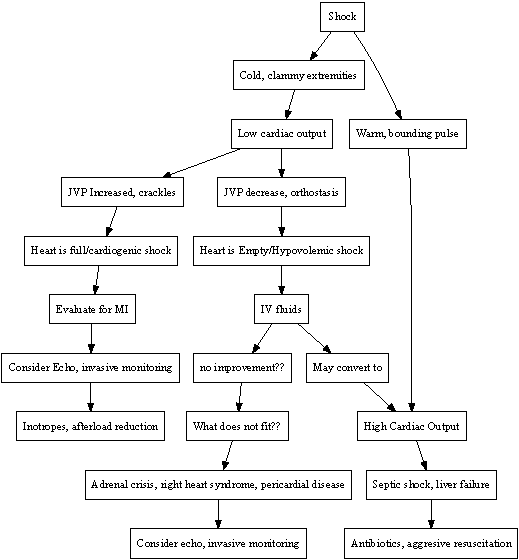
\includegraphics{critical_care_files/figure-pdf/fig-shockalgorithm-1.pdf}

}

\caption{\label{fig-shockalgorithm}Approach to Shock}

\end{figure}%

\subsection{Respiratory Failure}\label{respiratory-failure}

Respiratory failure mechanistically on the basis of pathophysiology can
be categorized onto:

\paragraph{Type 1: Acute Hypoxemic Respiratory
Failure}\label{type-1-acute-hypoxemic-respiratory-failure}

It occurs due to alveolar flooding, subsquent Ventilation-perfusion (VP)
mismatch and intrapulmonary shunt physiology.

Alveolar flooding occurs due:

\begin{itemize}
\tightlist
\item
  pulmonary edema, pulmonary edema further caused by:

  \begin{itemize}
  \tightlist
  \item
    elevated pulmonary microvascular pressures (heart failure or fluid
    overload) or
  \item
    ARDS (low pressure pulmonary edema), defined as: acute onset
    (\(\le\) 1 week) of bilateral opacities on chest imaging that are
    not fully explained by cardiac failure or fluid overload and
    ventilation perfusion mismatch, and shunt physiology that require
    positive end-expiratory pressure (PEEP)
  \end{itemize}
\item
  lung injury
\item
  pneumonia
\item
  alveolar hemorrhage
\end{itemize}

Type 1 RF occurs in sepsis, gastric aspiration, pneumonia, covid-19,
near drowning, multiple blood transfusion \& pancreatitis.

\subparagraph{General Treatment}\label{general-treatment}

\begin{itemize}
\item
  Mechanical ventilation. Mechanical ventilation with high tidal volume
  (12 ml/kg ideal body weight) traditionally further injured the lung
  due to repeated alveoli overdistention and stretching. This is called
  ventilator induced volutrauma and even induce ARDS in patients without
  ARDS initialy. many studies point toward low tidal volume (6 ml/kg
  ideal body weight) improve survival.

  reproduce Figure of Preassure volume relathionsip!!!
\item
  Prone positioning
\item
  Low CVP or low PCWP or fluid conservatice approach fluid conservative
  management to maintain low CVP or PCWP associated with fewer days with
  mechanical ventilation than fluid liberal approach in patients that
  who have been resuscitated from shock.
\end{itemize}

\paragraph{Type 2 Respiratory Failure: Hypercapnic Respiratory
Failure}\label{type-2-respiratory-failure-hypercapnic-respiratory-failure}

It is a consequence of alveolar hypoventilation and the results from
inability to eliminate CO2 effectively. The cause categorized into:

\begin{itemize}
\item
  impaired CNS drive to breathe (``wont breathe'') Cause: drug overdose,
  brainstem injury, sleep-disordered breathing, severe hypothyroidism
\item
  reduced strength or impaired neuromuscular function in respiratory
  systems (``cant breathe'') cause: impaired neuromuscular transmission
  (eg. myasthenia gravis, Guillain-Barre syndrome, amyotrophic lateral
  sclerosis) or respiratory muscle weakness (eg. myopathy, electrolye
  problem, fatigue)
\item
  increased load on respiratory system (``cant breathe'') cause:

  \begin{itemize}
  \item
    increased resistive load eg. brochospasm
  \item
    reduced lung compliance eg. alveolar edema, atelectasis, intrinsip
    PEEP
  \item
    reduced chest wall compliance eg. pneumothorax, pleural effusion,
    abdominal distention
  \item
    increased minute ventilation requirements eg. pulmoanry embolus with
    increased dead space fraction, sepsis
  \end{itemize}
\end{itemize}

\subparagraph{general Treatment}\label{general-treatment-1}

Principal: reversing the underlying cause(s). Non-invasive ventilation
(NIV) with positive pressure ventilation with tight fitting mask or
nasal mask (avoidance of intubation) may stabilize these patients. It
tested extensively in exacerbation of COPD. Contraindication for NIV
include hemodynamic instability, inability to protect airway,
respiratory arrests, significant airway secretions, significant
aspiration risk.

\paragraph{Type 3 Respiratory Failure: Lung
Atelectasis}\label{type-3-respiratory-failure-lung-atelectasis}

The primary cause is lung atelectasis. It is common in perioperaticve
period, this form is also called perioperative respiratory failure. Post
general anesthesia, there are decrease in functional residual capacity
lead to collapse of dependent lung units.

\subparagraph{general treatment}\label{general-treatment-2}

treatment include: frequent positional changes, chest physiotherapy,
upright positioning, control of incisional/or abdominal pain.

\paragraph{Type 4 Respiratory Failure: Metabolic
Demands}\label{type-4-respiratory-failure-metabolic-demands}

Most often due to hypoperfusion of respiratory muscles in patients in
shock. Normally, respiratory muscle consume \textless{} 5\% total
cardiac outpur (CO) and oxygen delivery. Patients in shock oftern
experience respiratory distress due to pulmonary edema (eg. in
cardiogenic shock), lactic acidosis and anemia. In these conditions, up
to 40\% CO distributed to respiratory muscle.

\subparagraph{General Treatment}\label{general-treatment-3}

Endotrachea intubation \& mechanical ventilation allow blood
redistributed to vital organ and reverse the underlying cause.

\subsubsection{Mechanical Ventilation}\label{mechanical-ventilation}

mechanical ventialtion is used to assist or replace sponstaneus
breathung. Its application of high oxygen content + positive pressure.
Primary indication is \textbf{acute respiratory} failure which there are
two basic types: 1. hypoxemic and 2. hypercarbic. \emph{Hypoexemic}
present when arterial O2 saturation \textless90\% despite increased
inspired O2 fraction due to ventilation perfusion mismatch or shunting.
\emph{Hypercarbic} characterized by elevated arterial CO2 (usually
\textgreater50 mmHg) resulting from conditions that decrease minute
ventilation or increased physiologic dead space.

\paragraph{Types of Mechanical
Ventilation}\label{types-of-mechanical-ventilation}

there are two types of MV: noninvasive ventilation (NIV) and invasive
(conventional MV)

\subparagraph{Noninvasive ventilation}\label{noninvasive-ventilation}

NIV: effective in acute and chronic respiratory failure with fewer
complication (pneumonia \& tracheolaringeal trauma). NIV provided by
tight fitting mask, a nasal mask similar to taht used for sleep apnea.
It is especially effective in COPD. Modes used are bilevel positive
airway pressure (BiPAP) or pressure support ventilation (PSV). Both used
positive pressure during inspiration and expiration, althouhg lower in
expiration. Trial showed: COPD exacerbation ph 7,25 - 7,35 associated
with good outcomes, for ph \textless7,25 the failure increase with
decreasing ph. patient with ph \textgreater7,35 NIV is not better than
conventional treatment (controlled O2, systemic glucocorticoid,
bronchodilator and antibiotics).

THe used of NIV in other respiratory failure is limited, and in some
conditions contraindicated (cardiac arrest, respiratory arrest,
decreased consciousness, GI bleeding, hemodynamic instability, MI,
facial trauma, upper airway obstruction, inability to clear secretion),
and may delay life saving measure. Reduced respiratory rate, decreased
the use of accesory muscle (scalene, sternomastoid and intercostal) are
good clinical indicator of improvement. ABG should be evaluated hours
after NIV initiation, if no improvement it may need a conventional MV

\subparagraph{Invasive Ventilation (Conventional
MV)}\label{invasive-ventilation-conventional-mv}

Intubation (cuffed tibed inserted to trachea) to allow conditioned
(warmed, oxygenated, humidified) gas delivered to the airways.

Principles of MV: optimize oxygenation while avoiding ventilator-induced
lung injury due to overstretch and collapse/re-recruitment (protective
ventilatory strategy)

\paragraph{Modes of Ventilation}\label{modes-of-ventilation}

modes are the manner in which breaths are triggered, cycled and limited.
- trigger: inspiratory effort or time based signal - cycle : refers to
the factors that determine the end of inspiration (volume, pressure and
time cycling) - limiting factors are operator-specified values: airway
pressure.

Most patient ventilated with assist-control, intermittent mandatory
ventilation, PSV.

\subparagraph{Assist control
ventilation}\label{assist-control-ventilation}

Assist control (ACMV) is the most widely used. Used in initiation of MV.
trigger: initiated by patient inspiratory effort, if none detected, by
specified time signal. cycle: pressure or volume cycle. limit: specified
tidal-volume, RR defined by patients rate or backup rate.

problem: auto-peep might occurs if dynamic hyperinflation due to high RR
happens.

\subparagraph{Intermittent Mandatory
Ventilation}\label{intermittent-mandatory-ventilation}

Most commmon modes: SIMV trigger: set mandatory breath, between each
mandatory breath patient can breath spontaneously. in SIMV, mandatory
breath delivered in syncrony with patients breath.if patient fail to
initiate a breath, the machine give fixed volume and reset its timer for
next breath. cycle: defined volume, limit:

difference with ACMV: only the a preset number of breath are
ventilator-assisted. SIMV allowd patients with intact respiratory drive
to exercise inspiratory msucles between assisted breath, useful for
supporting and weaning intubation. problem: difficult to use in
tacypnea, due to expiration attemp during ventilator inspiratory cycle.
The pressure increase, and may abort the inspiration and thus lower
tidal volume. In contrast, for tachypnea represent of metabocl or
respiratory acidosis, change in ACMV will increase minute ventilation
and help normalize pH

\subparagraph{Pressure-support
Ventilation}\label{pressure-support-ventilation}

trigger: patient breath cycle: flow, isnpiration is terminated when
airflow fall below a certain level. limit: pressure

provides graded asistence and differs from the other two in that the
operator set the pressure level to augment every spontaneous breath. The
level of pressure is adjusted by observing the patiens RR.

\subparagraph{Pressure-Control Ventilation
(PCV)}\label{pressure-control-ventilation-pcv}

useful to limit peak pressure, in patients with preexisting barotreauma
or post htoracic surgery.

trigger: time cycle: time, limit: pressure

minute ventilation is altered through RR and pressure control.

\subparagraph{Continous Positive Airway Pressure
(CPAP)}\label{continous-positive-airway-pressure-cpap}

All ventilation occurs through the patients spontaneus efforts. The
machine provide fresh gas to the circuit and set constant pressure.

\paragraph{Protective Ventilatory
Strategy}\label{protective-ventilatory-strategy}

Whatever the modes of MV, the principles:

\begin{enumerate}
\def\labelenumi{\arabic{enumi}.}
\tightlist
\item
  Set target tidal volume close to 6 ml/kg of ideal body weight
\item
  Prevent plateu pressure exceed 30 cm H\textsubscript{2}O
\item
  Use the lowest possible FIO\textsubscript{2} to keep
  SaO\textsubscript{2} \(\ge\) 90\%
\item
  Adjust the PEEP to maintain alveolar patency while preventing
  overdistention and closure/reopening.
\end{enumerate}

\paragraph{Maintenance for mechanical Ventilated
patients}\label{maintenance-for-mechanical-ventilated-patients}

\textbf{Respiratory System Mechanics}

Peak airway pressure dtermined by two variable: airway resistance and
respiratory system compliance. At the end of inspiration, there are
transient pause of inspiratory flow, the pressure called plateu
pressure. Plateu pressure determined by respiratory system compliance.
During volume controlled ventilation, the difference peak airway
pressure (airway + respiratory system) and plateu pressure (respiratory
system) provides a quantitative assesment of airway resistance. Patients
with increased airway resistence typically have increased peak airway
pressures and abnormally high gradients between peak and plateu airway
pressure (\textgreater{} 10 - 15 cmH\textsubscript{2}O) at a constant
inspiratory flow rate of 1 L/s(shown in figure
Figure~\ref{fig-airwayresistance}. Normally, respiratory system
compliance is \textasciitilde{} 100 ml/cmH\textsubscript{2}O, divided by
the lungs and chest wall. Pathophysiologic process decrease wall
compliance such as pleural effusion, pneumothorax \& increase abdominal
girth. Lung compliance decreased by pneumonia, pulmonary edema, alveolar
hemorrhae, interstitial lung disease, or auto PEEP. Auto-PEEP occurs
when there is insufficient time for emptying of alveoli before the next
inspiratory cycle, thus alveoli failed to decompress fully and remains
positive pressure at all phase of respiration. Theis phenomenon results
most commonly from obstruction of distal airways such as Asthma or COPD.

\begin{figure}

\centering{

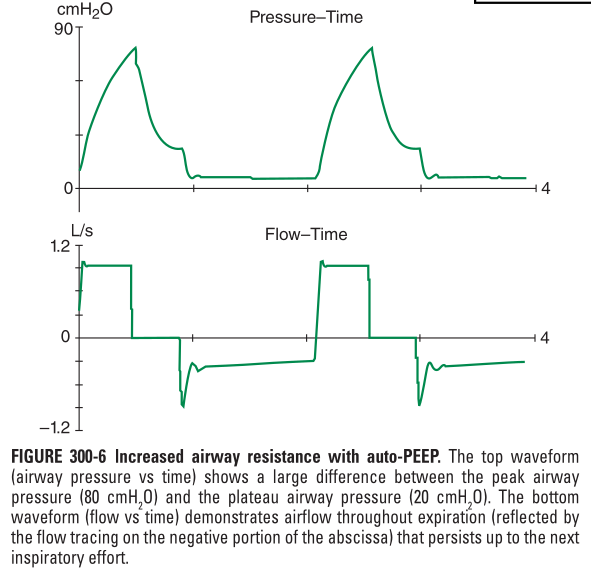
\includegraphics{Airway_resistance.png}

}

\caption{\label{fig-airwayresistance}Graph Illustration taken from
harrison}

\end{figure}%

Patients frequently require sedatives \& analgetics.

\subparagraph{Analgesics}\label{analgesics}

Opieates is the mainstay of mechanicaly ventilated patients

\subparagraph{Sedatives}\label{sedatives}

After pain adequately controlled, sedation needed for anxiolysis,
treatment of subjective dyspnea, reduction of autonomic hyperactiviy,
reduction of total O2 consumption. Nonbenzodiazepin are preffered
because benzodiazepin associated with increased delirium and worse
patients outcome.

Amnesia could be achieved with propofol or benzodiazepine such lorazepam
or midazolam.

\subparagraph{Neuromuscular Blocking
Agents}\label{neuromuscular-blocking-agents}

Patients with ventilatory dyssyncrony despite optimal sedation may
needed paralytics agents. Wathout for prolonged weakness, a myopathy
known as the postparalytics syndrome. Thus, neuromuscular blocking is
the last agent, only in patients which fail to achieve ventilator
syncrony with aggresive sedation. Remember, neuromuscular blocking agent
do not results in pharmacological paralysis without altering mental
status, thus sedative is almost always required for amnesia.

\paragraph{Ventilator Weaning and
Extubation}\label{ventilator-weaning-and-extubation}

Recognition of patients readyness to be liberated from mechanical
ventilation is important. Screening conducted daily, criteria:

\begin{enumerate}
\def\labelenumi{\arabic{enumi}.}
\tightlist
\item
  Stable oxygenation (Pao\textsubscript{2} / Fio\textsubscript{2}
  \textgreater{} 200 and PEEP \(\le\) 5 cm H\textsubscript{2}O)
\item
  Cough and Airway Reflexes Intact
\item
  No Vasopressor administered
\item
  No Sedatives adminsitered
\end{enumerate}

if all requirement passed, patient should undergi a spontaneous
breathing trial (SBT), if sedative still administered, patients could
also undergo spontaneous awakening trial (SAT.

SAT/SBT trial consist of a period of breathing through endotracheal tube
with little or without ventilator support (CPAP 1-5
cmH\textsubscript{2}O with or without low-level pressure support (PSV)
and open T-piece breahing system) for 30 - 120 minutes. SBT Failure or
should be stopped if:

\begin{enumerate}
\def\labelenumi{\arabic{enumi}.}
\tightlist
\item
  RR \textgreater35 min for \textgreater5 min
\item
  O\textsubscript{2} saturation \textless90\%
\item
  HR \textgreater{} 140x/min or a 20\% increase or decrease from
  baseline
\item
  SBP \textless90 mmHg or \textgreater180 mmHg
\item
  Increased anxiety or diaphoresis
\end{enumerate}

if none of these events occured, patients should considered for an
extubation trial. Despite these carefull criteria, 10\% patients develop
respiratory distress after extubation and may require resumption of
mechanical ventilation and reintubation.

Once patients determined that able to breath spontaneously, then
proceeed to remove the artificial airway which should be undertaken only
when it is patients showed the ability to protect airway, able to cough
and clear secretions, alert enough to follow commands. If reintubation
is deemed difficult if required, evaluation with cuff-leak test is
supported by evidence. If possibility of post-extubation stridor,
administration of systemic steoroid should be given.

\subsubsection{Prolonged MV and
Tracheostomy}\label{prolonged-mv-and-tracheostomy}

5-13 \% patients with MV will go on to require prolonged MV
(\textgreater21 days). It is important to decide whether and when to
perform a trachoestomy. Tracheostomy is though to be more comfortable,
require less sedation, and provide a more secure airway and reduce
weaning time.

In general, if a need of MV for \textgreater10-14 days, a tracheostomy
would be indicated.

\paragraph{Maintenance for mechanical Ventilated
patients}\label{maintenance-for-mechanical-ventilated-patients-1}

\textbf{Respiratory System Mechanics}

Peak airway pressure dtermined by two variable: airway resistance and
respiratory system compliance. At the end of inspiration, there are
transient pause of inspiratory flow, the pressure called plateu
pressure. Plateu pressure determined by respiratory system compliance.
During volume controlled ventilation, the difference peak airway
pressure (airway + respiratory system) and plateu pressure (respiratory
system) provides a quantitative assesment of airway resistance. Patients
with increased airway resistence typically have increased peak airway
pressures and abnormally high gradients between peak and plateu airway
pressure (\textgreater{} 10 - 15 cmH\textsubscript{2}O) at a constant
inspiratory flow rate of 1 L/s(shown in figure
Figure~\ref{fig-airwayresistance}. Normally, respiratory system
compliance is \textasciitilde{} 100 ml/cmH\textsubscript{2}O, divided by
the lungs and chest wall. Pathophysiologic process decrease wall
compliance such as pleural effusion, pneumothorax \& increase abdominal
girth. Lung compliance decreased by pneumonia, pulmonary edema, alveolar
hemorrhae, interstitial lung disease, or auto PEEP. Auto-PEEP occurs
when there is insufficient time for emptying of alveoli before the next
inspiratory cycle, thus alveoli failed to decompress fully and remains
positive pressure at all phase of respiration. Theis phenomenon results
most commonly from obstruction of distal airways such as Asthma or COPD.

\begin{figure}[H]

{\centering 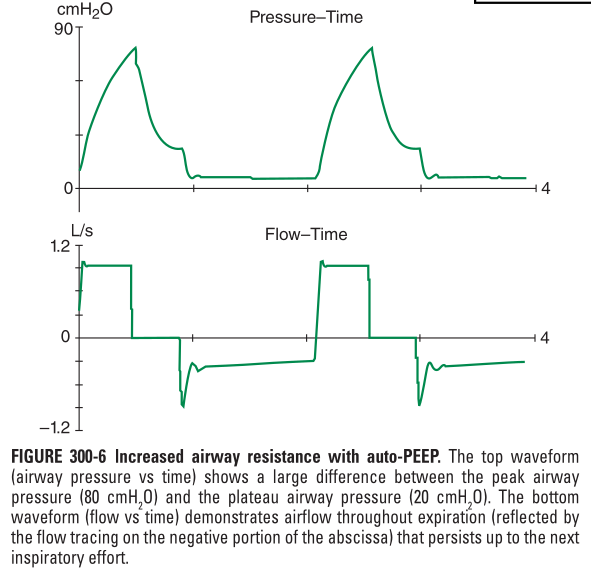
\includegraphics{Airway_resistance.png}

}

\caption{Graph Illustration taken from harrison}

\end{figure}%

Patients frequently require sedatives \& analgetics.

\subparagraph{Analgesics}\label{analgesics-1}

Opieates is the mainstay of mechanicaly ventilated patients

\subparagraph{Sedatives}\label{sedatives-1}

After pain adequately controlled, sedation needed for anxiolysis,
treatment of subjective dyspnea, reduction of autonomic hyperactiviy,
reduction of total O2 consumption. Nonbenzodiazepin are preffered
because benzodiazepin associated with increased delirium and worse
patients outcome.

Amnesia could be achieved with propofol or benzodiazepine such lorazepam
or midazolam.

\subparagraph{Neuromuscular Blocking
Agents}\label{neuromuscular-blocking-agents-1}

Patients with ventilatory dyssyncrony despite optimal sedation may
needed paralytics agents. Wathout for prolonged weakness, a myopathy
known as the postparalytics syndrome. Thus, neuromuscular blocking is
the last agent, only in patients which fail to achieve ventilator
syncrony with aggresive sedation. Remember, neuromuscular blocking agent
do not results in pharmacological paralysis without altering mental
status, thus sedative is almost always required for amnesia.

\paragraph{Ventilator Weaning and
Extubation}\label{ventilator-weaning-and-extubation-1}

Recognition of patients readyness to be liberated from mechanical
ventilation is important. Screening conducted daily, criteria:

\begin{enumerate}
\def\labelenumi{\arabic{enumi}.}
\tightlist
\item
  Stable oxygenation (Pao\textsubscript{2} / Fio\textsubscript{2}
  \textgreater{} 200 and PEEP \(\le\) 5 cm H\textsubscript{2}O)
\item
  Cough and Airway Reflexes Intact
\item
  No Vasopressor administered
\item
  No Sedatives adminsitered
\end{enumerate}

if all requirement passed, patient should undergi a spontaneous
breathing trial (SBT), if sedative still administered, patients could
also undergo spontaneous awakening trial (SAT.

SAT/SBT trial consist of a period of breathing throung endotracheal tube
without ventilator support (CPAP 5 cmH\textsubscript{2}O with or without
low-level pressure support and open T-piece breahing system) for 30 -
120 minutes. SBT Failure or should be stopped if:

\begin{enumerate}
\def\labelenumi{\arabic{enumi}.}
\tightlist
\item
  RR \textgreater35 min for \textgreater5 min
\item
  O\textsubscript{2} saturation \textless90\%
\item
  HR \textgreater{} 140x/min or a 20\% increase or decrease from
  baseline
\item
  SBP \textless90 mmHg or \textgreater180 mmHg
\item
  Increased anxiety or diaphoresis
\end{enumerate}

if none of these events occured, patients should considered for an
extubation trial. Despite these carefull criteria, 10\% patients develop
respiratory distress after extubation and may require resumption of
mechanical ventilation and reintubation.

\subsection{Multiorgan system failure}\label{multiorgan-system-failure}

Multiorgan system failure, defined by the simultaneous presence of
physiologic dysfunction and/or failure of two or more organs. Organ
failure, no matter how it is defined must persist beyond 24 hours.

\section{Specific Critical illness}\label{specific-critical-illness}

\subsection{Acute Respiratory Distress Syndrome
(ARDS)}\label{acute-respiratory-distress-syndrome-ards}

ARDS is clinical syndrome of \textbf{severe dyspnea} of rapid onset,
\textbf{hypoxemia}, and \textbf{diffuse pulmonary infiltrates} leading
to respiratory failures.

\subsection{Diagnostic Criteria for
ARDS}\label{diagnostic-criteria-for-ards}

\begin{longtable*}{llll}
\toprule
Severity (PaO2/FiO2) & Onset & Chest Radiograph & Absence of Left Atrial Hypertension \\ 
\midrule\addlinespace[2.5pt]
mild: 200 mmHg< X  <=300 mmHg; moderate: 100 mmHg < X <=200 mmHg; Severe: <= 100 mmHg & Acute: within 1 week of clinical insult or new, or worsening respiratory symptoms & Bilateral opacities consistent with pulmonary edema not fully explained by effusion, lobat/lung collapse, or nodules & Hydrostatic edema is not the primary cause of Respiratory Failure \\ 
\bottomrule
\end{longtable*}

ddx: - cardiogenic pulmonary edema - bilateral pneumonia - alveolar
hemorrhage

\subsection{Epidemiology}\label{epidemiology}

Estimated incidence: 60/100.000 population.

\subsubsection{Etiology}\label{etiology}

ARDS can be caused by diffuse lung injury from many medical and surgical
disorders. It may be direct (on the lung) or indirect (extrapulmoner
including thoracic structure). The most case (\textgreater80\%) are
caused by pneumonia and sepsis. Then, gastric aspiration, trauma,
multiple transfusiion, pancreatitis, and drug overdose. Traumatic cause
include pulmonary contusion, multiple bone fractures, chest trauma/flail
chest. The risk increase with predisposing medical condition.

\subsubsection{Pathophysiology}\label{pathophysiology}

Natural history of ARDS divided into 3 phases - exudative,
proliferative, and fibrotic.

\paragraph{Exudative Phase}\label{exudative-phase}

This phase encompases the first 7 days after precipitating ARDS risk
factor. The alveolar capillary endhotelial cells and type 1 pneumocytes
injured, loss of tight alveolar barrier to fluid and macromolecules.
Edema fluid contain protein accumulates in the interstitial and alveolar
spaces. Proinflamatory cytokines increase followed by leukocytes
recruitment. The leaked plasma condensed and agrreagte in the air spaces
+ cellular debris + dysfunctional surfactant to form hyaline membran
whorls.

Alveolar edema predominantly involves dependent portions of the lung
with diminished aeration. Large lung dimineshed aeration cause increase
in lung compliance. Alteration in alveolar spaces are exacerbated by
microvascular occlusion leading to reduced perfusion and pulmonary
hypertension. it also cause intrapulmonary shunting and hypoxemia,
leading to dyspnea.

sign: - dyspnea, may leads to respiratory fatigue - chest radiograph
reveals opacities resembling pulmonary edema. distinguishing featues
from cardiogenic pulmonary edema are no cardiomegaly, no pleural
effusin, or no pulmonary vascular redistribution. - laboratory finding
indicative of the underlying disoder.

\paragraph{Proliferative Phase}\label{proliferative-phase}

phase day 7 to 21. May showed an improvement, including weaning of
mechanical ventilation. It may shows some degree of lung repair, reduced
alveolar exudates, and shift to lymphocytes predominant infiltrat,
increased surfactant.

sign: - improvement in symtoms, but still dyspnea - tachypnea -
hypoxemia

\paragraph{Fibrotic Phase}\label{fibrotic-phase}

Phase 3-4 weeks after lung injury. Many patients may recover, but some
enter a fibrotic phase. The exudate convert to extensive alveolar duct
and interstitial fibrosis. desctruction of acinar architecture leads to
emphysema like changes (bullae), and may also develop microvascular
occlusion and pulmonary hypertension.

\subsubsection{Treatment}\label{treatment}

\paragraph{General Principles}\label{general-principles}

Emphasize on treatment of the Critical ill

\begin{enumerate}
\def\labelenumi{\arabic{enumi}.}
\tightlist
\item
  treatment of underlying cause
\item
  minimization of unnecessary procedures
\item
  standardized bundle care
\item
  promt recognition of nosocomial infections
\item
  adequte nutrition
\end{enumerate}

\begin{figure}

\centering{

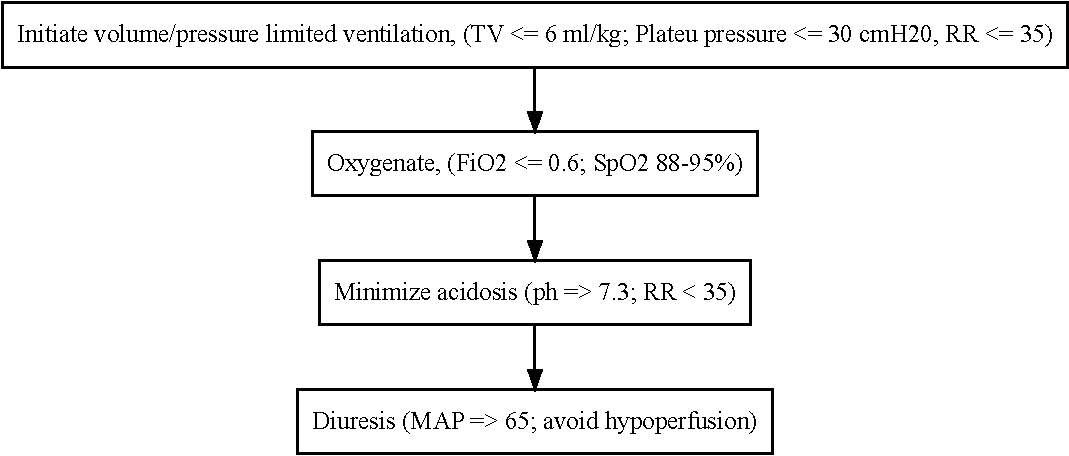
\includegraphics{critical_care_files/figure-pdf/fig-ardsalgorithm-1.pdf}

}

\caption{\label{fig-ardsalgorithm}ARDS Algorithm}

\end{figure}%

\paragraph{Mechanical Ventilation}\label{mechanical-ventilation-1}

Patient meeting criteria ARDS frequently become respiratory fatigues, so
it requires mechanical ventilation.

\subparagraph{Minimize ventilator induced lung
injury}\label{minimize-ventilator-induced-lung-injury}

Mechanical ventilatio (MV) can save lifes, but also can aggravate lung
injury due to volutrauma and atelectrauma. Volutrauma can occurs due to
overdistention of alveoli due to effort to inflate the consolited lungs
thus damaging the still functioning alveoli.

\begin{itemize}
\tightlist
\item
  \textbf{Low tidal volume 6ml/kg predicted body weight are better than
  coenventional 12 ml/kg bodyweight.}
\item
  lower airway pressure, plateu pressure \(\le\) 30 cm
  H\textsubscript{2}O.
\item
  RR \(\le\) 35
\end{itemize}

\subparagraph{Minimize atelectrauma}\label{minimize-atelectrauma}

In presence of fluid and loss of surfactant, PEEP is required to prevent
atelectasis. PEEP is adjusted to minimize FIO\textsubscript{2} while
able to provide adequate PaO\textsubscript{2} without causing alveolar
overdistention. Follow table of PEEP-FiO\textsubscript{2} combinations
from ARDS Network trial.

other technique includes \textbf{recruitment manuever}, that transiently
increase PEEP to high levels to recruit ateletatic lung can increase
oxygenation, but a mortality benefit has not been established.

\subparagraph{Prone positioning}\label{prone-positioning}

It improves survival.

\paragraph{Fluid Management}\label{fluid-management}

increased pulmonary vascular permeability leading to interstitial and
alveolar edema fluid rich in protein is a centra features of ARDS.
impaired vascular integrity augments the normal increase in
extravascular lung water. Thus keeping low left atrial filling pressure
could minimize pulmonary edema. Fluid restriction and diuretics should
be an important aspect of ARDS management, limited only by hypotension
and hypoperfusion.

\paragraph{Neuromuscular blockage}\label{neuromuscular-blockage}

Sedation alone may not adequate for ventilator syncrony. Selective use
of neuromuscular blockage for ventilator syncrony could improves
survival.

\paragraph{Glucocorticoids}\label{glucocorticoids}

Current evidence does not support the routine use of glucocorticoids.

\subsubsection{Prognosis}\label{prognosis}

extrapulmonary organ failures and sepsis counts \textgreater{} 80\% of
deaths. Risk factor for reduced survival are age (\textgreater60 yo),
preexistin organ dysfunction. Patients who survives despite prolonged
respiratory failures and dependent on MV may recover within 6 months.

\subsection{Approach to Circulatory
Shock}\label{approach-to-circulatory-shock}

shock is the clinical condition of organ dysfuntion resulting from
imbalance between celular oxygen supply and demand. Shock is reversible
in early state, but if left untreated leads to multisystem organ
dysfunction and death.

\subsubsection{Pathophysiology of Shock}\label{pathophysiology-of-shock}

The cellular oxygen imbalance most commonly related to impaired oxygen
delivery in the setting circulatory failure. - shock may also occurs in
the setting of failure oxygen utilization (cyanide poisoning) - and
state of increased oxygen demand.

In the setting of inadequate oxygen supply, the cell cannot maintain
aerobic metabolism, thus forced into anaerobic metabolism and produce
lactate and less ATP. Less ATP supply impaired cell ability to maintain
hemeostasis such as maintaining N/K pump. Celular pump failure cause
influx of calcium and leads to activation of phospolipases and protease,
causing cellular swelling and death. In addition, hypoxia cause leakage
of intracellular contents to the extracellular space, activating
inflamatory cascasdes.

Oxygen delivery influenced by two major components, namely Cardiac
Output (CO) and arterial oxygen content (CaO\textsubscript{2}.

DO\textsubscript{2} = CO x CaO\textsubscript{2}, major determinants of
CO are HR and SV

DO\textsubscript{2} = (HR x SV) x CaO\textsubscript{2}, major
determinants of SV are preload, afterload (SVR), and cardiac
contractility. thus

SV \textasciitilde{} (Preload x Contractility)/SVR

Preload refees to myocardical fibers lenght before contraction (LV-EDV).
Contractility refers to the ability of the ventricile to contract
independent of preload and afterload. SVR represent afterload, force
that ventricle must overcome to send the blood out of the cardiac
cambers.

The CaO\textsubscript{2} is composed of oxygen carried by convection
with hemoglobin and oxygen dissolved in blood,

CaO\textsubscript{2} = (Kg x 1,39 x SaO\textsubscript{2}) +
(PaO\textsubscript{2} x 0,03)

A disease process that affects these variables (HR, preload,
contractility, SVR, SaO2, or Hb) has potential to reduce
DO\textsubscript{2}.

\subsubsection{Classification of Shock}\label{classification-of-shock}

Four major shock types are distributive, cardiogenic, hypovolemic, and
obstrictive. Each has unique hemodynamics profile.

\paragraph{Distributive Shock}\label{distributive-shock}

Distributive shock is condition of reduced O\textsubscript{2} delivery
where the primary physiologic distubance is \textbf{reduction in SVR}.
There are \textbf{increase of CO} as a compensatory effort. CVP and PCWP
reduced. The most common etiology is sepsis. Sepsis is life-threatening
organ dysfunction due to dysregulated host response to infection. If
accompanied by persistent hypotension despite adequate fluid
resuscitation and needed vasopressor support, it is called septic shock.
Other medical cause : Anaphylaxis (IgE mediated vasodilatation after
exposure to allergen), pancreatitis, severe burns, liver failure. There
almost 35\% extravasation of circulating blood volume within 10 minutes.
Patiens with severe brain or spinal cord injury may have a reduction in
SVR due to disruption of autonomic pathways and blood pooling in venous
system. Other cause is adrenal insuficiency due to chronic steroid use,
medication , malignancy, adrenal hemmorhage, infection or autoimune.
Acute stress condition, created deficit in steroid, and cause
vasodilatation as well as aldosteron deficiency-mediated hypovolemia.

\paragraph{Cardiogenic Shock}\label{cardiogenic-shock}

Cardiogenic shock is characterized by reduced O\textsubscript{2}
delivery related to a reduction in CO owing to a primary cardiac
problem. There are compensatory response as an increase in SVR. If left
ventricle is dysfunction, there will be increased PCWP, and if right
ventricle is will present as increased CVP. SV may reduced due to
reduced contractility (MI, Cardiomyopathies, myocarditis), valvular
disease, or due to alteration in HR (bradiaritmia and tachyarithmia)

\paragraph{Hypovolemic Shock}\label{hypovolemic-shock}

Hypovolemic shock encompasses disease that reduce CO and
DO\textsubscript{2} via a reduction in preload. There is elevation is
SVR and low CVP-PCWP. Most common cause is hemmorhage followed by fluid
loss from diarhea or vomiting, diuresis, skin damage.

\paragraph{Obstructive Shock}\label{obstructive-shock}

Obstructive shock is reduced O\textsubscript{2} delivery related to
reduced CO because impairment in blood flow, both inflow and outflow, in
extracardiac pulmonary vascular or other mechanical process. Inflow
obstruction Etiology: tension pneumothorax, cardiac tamponade,
restrictive pericarditis. Outflow obstruction etiology: pulmonary
embolism, venous air embolis, fat embolism or aortic dissection.

UGD =\textgreater{} hypovolemic (30,8\%) \textgreater{} septic (27,2\%)
\textgreater{} distributive non septic (23,4\%) \textgreater{}
cardiogenic (14\%) \textgreater\textgreater\textgreater\textgreater{}
obstructiove shock (0,9\%). ICU =\textgreater{} Shock predominates
)62\%) \textgreater\textgreater{} Hypovolemic (16\%) \textasciitilde{}
cardiogenic shock (15\%) \textgreater\textgreater\textgreater{}
obstructive shock (2\%).

Mortality rate: cardiogenic \textasciitilde{} septic \textgreater{}
hypovolemic

\subsubsection{Stages of Shock}\label{stages-of-shock}

There are 3, preshock, shock and irreversible shock. Body utilize
variety of physiologic response to counter initial insult. There no
overt sign of organ dysfunction. Lab: slight elevation of creatine or
troponin or mild elevation of lactate. If host compensatory mechanism
are not enough, organ dysfuction occurs and irreversible Shock ensued.

\subsubsection{Evaluation of the patient with
Shock}\label{evaluation-of-the-patient-with-shock}

early recongition is paramount important to reverse the stages of shock.
Anamnesis to find the cause. Physical examination to identify
circulatory failure (hypotension SBP \textless90 mmHG, or MAP
\textless{} 65 mmHg) and sign of organ dysfunction. Check urine output.
Finding: High CO shock: warm peripherals, CRT \textless2 S, large pulse
pressure (LOW DBP). Low CO shock: delayed CRT, cool extremities, weak
pulses.

Increased instravasular filling pressure and JVP (cardiogenic,
obstrctive shock)

\textbf{Shock Index} : defined as the HR/SBP with normal SI 0,5 - 0,7

Lab test: - Lactate - Renal function - liver function - cardiac enzymes
- CBC - Hemostatic index - UL - PP test if needed - ECG - CXR - POCUS
(RUSH, ACES, SESAME protocol)

\subsubsection{Initial Treatment of
Shock}\label{initial-treatment-of-shock}

\paragraph{Initiate treatment for circulatory
shock.}\label{initiate-treatment-for-circulatory-shock.}

Find venous access and invasive monitoring if needed

\paragraph{Volume Resuscitation}\label{volume-resuscitation}

The physiologic goal of volume resuscitation is to move the patient to
the \textbf{nonpreload-dependent portion of the Starling curve}. Most
patients with any of the four shock types will benefit from an increase
in intra-vascular volume. suspected septic shock, a minimum of 30 mL/kg
is recommended by the Surviving Sepsis Campaign. While the need for
volume resuscitation is most apparent for patients with distributive or
hypovolemic shock, even patients with cardiogenic shock may benefit from
cautious volume replacement. In these patients, there should be a
careful assessment of volume status prior to volume administration.

Volume resuscitation will begin with \textbf{crystalloid}. In patients
with hypovolemic shock due to ongoing hemorrhage, volume replacement
with packed red blood cells is warranted. In cases of massive
transfusion, platelets and fresh frozen plasma should be provided to
offset the dilution of these components during volume replacement.
Because hemoglobin is a key determinant of CaCO2, \textbf{red cell
administration may be a part of volume replacement even without
hemorrhage in order to optimize oxygen delivery if hemoglobin content is
\textless7 g/dL.}

Assessment of intravascular volume status (and the adequacy of volume
resuscitation) begins with the physical examination. The \textbf{passive
leg raise (PLR) test can predict responsiveness to additional
intravenous fluid (IVF) by providing the patient with an endogenous
volume bolus.} While the patient is resting in a semirecumbent position
at a 45° angle, the bed is placed in Trendelenburg position such that
the patient's head becomes horizontal and the legs are extended at a 45°
angle. There is then an immediate (within 1 min) assessment of changes
in CO (or pulse pressure variation as a surrogate). It is important to
emphasize that one does not merely look for changes in blood pressure;
if the shock patient is mechanically ventilated there is the option of
looking at changes in \textbf{SV variation (or pulse pressure
variation)} during the respiratory cycle to assess volume
responsiveness. A \textgreater12\% SV variation suggests a
volume-responsive state. This measurement requires that the patient be
in a volume cycle mode of ventilation, without breath-to-breath
variations in intrathoracic pressure and without arrhythmias.

There is also increased use of echocardiography to assist in
determination of intravascular fluid status, with a variety of static
and dynamic variables The most commonly used parameters to assess
adequacy of volume resuscitation are inferior vena cava (IVC) diameter
and IVC collapse. Alternatively, serial assessments of LV function can
be performed while volume is being administered. Placement of a
pulmonary artery catheter (PAC) is another tool for assessment of volume
status. This more invasive measure involves placement of the PAC into
the central venous circulation and through the right heart. Ports in the
PAC (Swan-Ganz catheter) allow for direct measurement of CVP, pulmonary
artery (PA), and PCWPs. The PCWP is used as a surrogate for LA pressure.

\paragraph{Vasopresor and Inotropic
Support}\label{vasopresor-and-inotropic-support}

If hypotension and inadequate tissue perfusion persist, then vasopressor
and inotropic support should be initiated. \textbf{The use of
vasopressors and inotropes must be tailored to the primary physiologic
disturbance.}

In distributive shock, the aim is to increase the SVR.
\textbf{Norepinephrine is the first-choice vasopressor}, with potent α1
and β1 adrenergic effects. The α1 causes vasoconstriction while β1 has
positive inotropic and chronotropic effects. At high doses, epinephrine
has a similar profile (at lower doses the β effects predominate) but is
associated with tachyarrhythmia, myocardial ischemia, decreased
splanchnic blood flow, pulmonary hypertension, and acidosis. In
distributive shock, vasopressin deficiency may be present. Vasopressin
acts on the vasopressin receptor to reverse vasodilation and
redistribute flow to the splanchnic circulation. \textbf{Dopamine does
not have a role as a first-line agent in distributive shock.}

For patients with \textbf{cardiogenic shock, dobutamine is the
first-line agent}; it is a synthetic catecholamine with primarily
β-mediated effects and minimal α adrenergic effects. The β1 effect is
manifest in increased inotropy and the β2 effect leads to vasodilation
with decreased afterload; it can be used with norepinephrine in patients
with mixed distributive and cardiogenic shock.

\paragraph{Oxygenation and Ventilation
Support}\label{oxygenation-and-ventilation-support}

Supplemental oxygen should be initiated and titrated to maintain SpO2 of
92--95\%. patients may require intuvation and MV for two reason:

\begin{enumerate}
\def\labelenumi{\arabic{enumi}.}
\item
  primary pulmonary process or related to LV dysfunction and elevations
  of PCWP. For patients with all types of shock, there can be
  development of ARDS and subsequent V/Q mismatch and shunt.
\item
  high minute ventilatory needs to compensate for metabolic acidosis. As
  shock progresses, they may not be able to maintain adequate
  respiratory compensation.
\end{enumerate}

It is important to provide ventilation with lung-protective strategies
focused on low tidal volume ventilation and optimization of positive
end-expiratory pressure to minimize ventilator-induced lung injury.

\paragraph{Antibiotics}\label{antibiotics}

For patients presenting with undifferentiated shock, if the diagnosis of
septic shock is being entertained, then broad-spectrum antibiotics
should be administered after obtaining appropriate cultures. While it is
ideal to initiate antibiotics after appropriate cultures, the inability
to obtain cultures should not delay the start of treatment

\paragraph{Other specific treatment for specific
etiology}\label{other-specific-treatment-for-specific-etiology}

The initial evaluation (history, physical examination, and diagnostic
testing) may have identified an etiology of shock that requires urgent
lifesaving intervention in addition to the initial treatment steps out-
lined above.

\subsection{Sepsis}\label{sepsis}

\subsection{Cardiogenic Shock and Pulmonary
edema}\label{cardiogenic-shock-and-pulmonary-edema}

\subsection{Cardiac Arrest}\label{cardiac-arrest}

\subsection{Neurological Critical
illness}\label{neurological-critical-illness}

\section{Important Calculation}\label{important-calculation}

\subsection{Airway \& Ventilation}\label{airway-ventilation}

\subsection{Circulation}\label{circulation}

\subsubsection{Oxygen Delivery}\label{oxygen-delivery}

Oxygen delivery (DO\textsubscript{2} or QO\textsubscript{2}) is a
function of cardiac output and the content of O\textsubscript{2} in the
arterial blood (CaO\textsubscript{2}). CaO\textsubscript{2} is
determined by HB concenctration, arterial HB saturation, and dissolved
O\textsubscript{2} disolved in plasma (not bound to HB). Equation
provided at Equation~\ref{eq-delivery-oxygen}. Nearly all oxygen
delivered to the tissue is bound to HB. Disolved O2 are negligible.

Arterial oxygen content (CaO\textsubscript{2}) normally around 21.16
mL/dL, while the mixed venous blood (VO\textsubscript{2}) is 15.76
mL/dL, thus normal tissue extraction is around 25\%. Reduced
VO\textsubscript{2} may results from inadequate CO, reduced HB or
reduced SaO\textsubscript{2}. Abnormally high VO\textsubscript{2} may be
caused by fever, agitation, shivering and thyrotoxicosis.

\begin{equation}\phantomsection\label{eq-delivery-oxygen}{
QO~2~ = \text{Cardiac Output} \text{ (dL/min)} \times (1.39 \times \text{HB concentration} \times \text{HB% Saturation} + 0.0031 \times PaO2)
}\end{equation}

\[
QO~2~ = 50 \text{ dL/min} \times (1.39 \times 15 \text{g/dL} \times 100\% + 0.0031 \times 100)
\] \[
QO~2~ = 50 \text{ dL/min} \times 21.6 \text{mL O2 per dL blood or CaO2} = 1058 \text{ mL O2 per min}
\]

\chapter{Hematology \& Medical
Oncology}\label{hematology-medical-oncology}

\section{Oncological Emergency}\label{oncological-emergency}

\section{Hematology}\label{hematology}

\subsection{Transfusion Medicine}\label{transfusion-medicine}

\section{Medical Oncology}\label{medical-oncology}

\section{Procedures in Hematology and Medical
Oncology}\label{procedures-in-hematology-and-medical-oncology}

\subsection{Examination of Blood Cells \& Marrow
Cells}\label{examination-of-blood-cells-marrow-cells}

\subsubsection{Examination of Blood
Cells}\label{examination-of-blood-cells}

\paragraph{Automated Quantitative
Parameter}\label{automated-quantitative-parameter}

Red cell parameter that measured directly: MCV, Red cell number,
hemoglobin concentration, and red cell distribution width. Parameter
derived from calculation: HCT, MCH, MCHC

\subparagraph{Measurement of RBC count and
hematocrite}\label{measurement-of-rbc-count-and-hematocrite}

HCT are measured from RBC x MCV/10, falsely elevated MCV and decreased
RBC can be observed when red cell autoantibodies are presents and
binding capability at room temperature, thus creatig red cell clumping.

\subparagraph{Measurement of
Hemoglobin}\label{measurement-of-hemoglobin}

RBC contain mixture of HB, including: oxyhemoglobin, carboxyhemoglobin,
methemoglobin, and other minor hemoglobin. HB quantification done lysing
the cell and converted the all HB variants to cyanmethemoglobin for
quantification by absorptio at 540 mm. Major interference with this
method is the present of chylomicronemia.

\subparagraph{Standard Red Cell
Indices}\label{standard-red-cell-indices}

\textbf{Mean Cell Volume}

Mean cell volume (MCV) are measured directly by electrical impendance or
light scattering.

\textbf{Mean Cell Hemoglobin}

Mean cell hemoglobin (MCH) is the amount of HB per red cell. It is
derived from Hemoglobin content and red cell count, two most accurate
measurement, thus could provide consistent result among many type of
analyzer. Reduced cell hemogobin is paralel to the reduced MCV. Mean
cell hemoglobin concentration is not used much for diagnostic, it is
primarily ised for quality control purpose.

\textbf{Red Cell Distribution Width}

Red cell distribution widht or RDW is an estimate of volume variability
in red cells population. RDW expressed as 1 SD of red cell volume
measurements divided by the MCV.RDW has developed as biomarker for
various clinical condition and may be a surrogate of systemic
inflamation

\textbf{Reticulocyte Count \& RNA Content}

Reticulocyte is a newly released anuclete red cell that enters
bloodstream with residual but detectable RNA. The Reticulocyte counts
permits an estimate of marrow erythrocyte production, thus provide tools
for evaluation anemia due to inadequate production or accelerated
destruction. Reticulocytes are now measured by exposig the samples with
Fluoresced, RNA binding Dyes. Measurement are reported in abosolute
counts, reticulosytes per microliter of Blood, obviating the need to
corrrect for reduced red cell counts in anemia.

The measuremet of Reticulocytes specific hemoglobin content (CHr and
RET-He) are closely related to iron availability withiin 24-48 hours,
and is very usefull in detecting functional iron deficiency in complex
clinical situation such as chronic inflamation or chronic kidney
disease. Reticulocytes specific hemoglobin are superior to traditional
iron parameter due to feritin also acts as a acute phase reactants.

\textbf{Other Indices}

Nucleated red cells: are presents in newborns, physiologicaly stress
individual and variety disorders such as hypoxic states, severe
hemolytics anemia, primary myelofibrosis, infiltrative disease of the
marrow.

\subparagraph{Leukocyte Counts and
Differetial}\label{leukocyte-counts-and-differetial}

\paragraph{Qualitative Parameter}\label{qualitative-parameter}

\subsubsection{Examination of Marrow
Cells}\label{examination-of-marrow-cells}

Bone marrow aspiration was devised by Arinkin in 1923, then the egular
use posterior illiac crest for aspiration and biopsy occured in 1970.

\chapter{Allergy \& Immunology}\label{allergy-immunology}

\chapter{Rheumatology}\label{rheumatology}

\chapter{Infectious Disease}\label{infectious-disease}

\section{Bacterial Infection}\label{bacterial-infection}

\section{Viral Infection}\label{viral-infection}

\subsection{HIV}\label{hiv}

\subsubsection{Imunopatogenesis HIV
Infection}\label{imunopatogenesis-hiv-infection}

\subsubsection{}\label{section}

\subsection{Dengue}\label{dengue}

\section{Fungal Infection}\label{fungal-infection}

\chapter{Cardiology \& Vascular
Medicine}\label{cardiology-vascular-medicine}

\chapter{Respiratory Medicine}\label{respiratory-medicine}

\chapter{Nefrology \& urology}\label{nefrology-urology}

\section{Nefrology}\label{nefrology}

\subsection{Hypertension}\label{hypertension}

\subsection{FLuid and Electrolyte
Disorders}\label{fluid-and-electrolyte-disorders}

\subsubsection{Disorders of Extracelular
Volume}\label{disorders-of-extracelular-volume}

\subsubsection{Disorders of Water
Metabolism}\label{disorders-of-water-metabolism}

\subsubsection{Disorders of Potassium
Metabolism}\label{disorders-of-potassium-metabolism}

The most frequent electrolyte abnormalities in clinical
medicine.Patients with disor-ders of potassium metabolism may be
asymptomatic, or they may have symptoms ranging from mild weakness to
sudden death.

\paragraph{Normal Physiology}\label{normal-physiology}

\subparagraph{Potassium Intake}\label{potassium-intake}

Potassium is necessary for essentially all cellular functions, is
present in most foods, and is excreted primarily by the kidney. Typical
diet 70 mmol of potassium, while the recommended intake is 120 mmol per
day. Gastrointestinal tract efficiently absorbs potassium.

\subparagraph{Potassium Distribution}\label{potassium-distribution}

After absorption from the GI tract, potassium distributes rapidly into
the extracellular fluid (ECF) and intracellular fluid (ICF)
compartments. Cellular potassium uptake is rapid and limits the
magnitude of changes in serum potassium concentration. During potassium
deficiency, shift of potassium from intracellular to extracellular
compartments limits the change in extracellular potassium concentration.

Most potassium is in the ICF. Most body potassium is intracellular, with
only 1\% to 2\% in the ECF. Potassium is the major intracellular cation,
with cytosolic K+ concentrations about 100 to 120 mmol/L. Total
intracellular K+ content is 3000 to 3500 mmol in healthy adults and is
found primarily in muscle (70\%), with a lesser amount in bone, red
blood cells, liver, and skin.

\subparagraph{Renal Handling of Potassium in Normal
Kidney}\label{renal-handling-of-potassium-in-normal-kidney}

\subparagraph{Renal Potassium Handling in Chronic Kidney
Disease}\label{renal-potassium-handling-in-chronic-kidney-disease}

\paragraph{Hypokalemia}\label{hypokalemia}

\paragraph{Hyperkalemia}\label{hyperkalemia}

\subsubsection{Disorders of Calcium, Phosphate and Magnesium
Metabolism}\label{disorders-of-calcium-phosphate-and-magnesium-metabolism}

\subsubsection{Acid-Base Balance}\label{acid-base-balance}

\paragraph{Metabolic Acidosis}\label{metabolic-acidosis}

\paragraph{Metabolic Alkalosis}\label{metabolic-alkalosis}

\paragraph{Respiratory Acidosis}\label{respiratory-acidosis}

\paragraph{Respiratory Alkalosis}\label{respiratory-alkalosis}

\paragraph{Mixed Acid Base Balance}\label{mixed-acid-base-balance}

\subsection{Infectious Disease in
Kidney}\label{infectious-disease-in-kidney}

\subsection{Acute Kidney Injury}\label{acute-kidney-injury}

\subsection{GLomerular Disease}\label{glomerular-disease}

\subsection{Tubulointerstitial
Disease}\label{tubulointerstitial-disease}

\subsection{Diabetic Kidney Disease}\label{diabetic-kidney-disease}

\subsection{Renovascular Disease}\label{renovascular-disease}

\subsection{Pregnancy and Renal
Disease}\label{pregnancy-and-renal-disease}

\subsection{Congenital Disease of the
Kidney}\label{congenital-disease-of-the-kidney}

\subsection{Chronic Kidney Disease}\label{chronic-kidney-disease}

\subsection{Dialytic Therapy}\label{dialytic-therapy}

\subsection{Transplantation}\label{transplantation}

\subsection{Edema and Diuretics use}\label{edema-and-diuretics-use}

\paragraph{Diuretics Type}\label{diuretics-type}

Diuretics are based on the sites of action. These are as follows:

\paragraph{Proximal Tubular Diuretics}\label{proximal-tubular-diuretics}

Carbonic Anhydrase inhibitor (CAI) work by inhibiting generation of
intracellular Hidrogen ion, which is a requirement for absorption of
natrium. This is the main action for its diuretics property. Most of the
work in proximal tubule where bulk of natrium absorption, although Na
absorption in more distal tubule will reduce CAI effects. Acetazolamide
is the only diuretics used in practice. Asetasolamide has short action,
due to ready absorbed and easily eliminated by tubular action. Prolonged
used will cause metabolic acidosis, thus acetazolamied 250 to 500 mg
daily used to correct metabolic alkalosis as side effects of thiazide or
loop diuretics. Its use shouldbe cautiously in advanced kidney disease
as it will systemically accumulates with repeat dosing.

\paragraph{Distal Convoluted Tubule
Diuretics}\label{distal-convoluted-tubule-diuretics}

\paragraph{Loop Diuretics}\label{loop-diuretics}

\paragraph{Distal Potassium-Sparing
Diuretics}\label{distal-potassium-sparing-diuretics}

\paragraph{Osmotic Diuretics}\label{osmotic-diuretics}

\subsubsection{Edema Treatment}\label{edema-treatment}

\section{Urology}\label{urology}

\chapter{Gastroenterology \&
Hepatology}\label{gastroenterology-hepatology}

\section{Gastroenterology}\label{gastroenterology}

\subsection{Anorectal Disease}\label{anorectal-disease}

composed of blood vessels, smooth muscle fibers, and supporting connec-
tive tissue, normally present in the anal canal. The term
``hem-orrhoids'' is also applied to situations when these cushions
become symptomatic.

Hemorrhoids are the result of slippage of the anal cushions due to
weakening of the supporting tissues. The prolapse hinders the venous flow
leading to dilatation and engorge-ment of the anal cushions, exposing
them to complications such as edema, thrombosis, and bleeding.

Hemorrhoids are classified as internal, external, or combined. Internal
hemorrhoids are located proximal to the dentate line and are covered by
insensate columnar mucosa or transitional epithelium. External
hemorrhoids are located below the dentate line, covered with squamous
epithelium rich in nerve endings.

\subsubsection{Clinical Presentation}\label{clinical-presentation}

The most common clinical presentation are;

\begin{enumerate}
\def\labelenumi{\arabic{enumi}.}
\tightlist
\item
  Bleeding per rectum.
\item
  Prolapsing tissue.
\end{enumerate}

Bleeding per rectum is The bleeding is bright red and painless, and it
usually follows evacuation.

Prolapse occurs during straining or heavy lifting causing dis-comfort,
feeling of incomplete evacuation, mucus discharge, and pruritus.
Prolapsing hemorrhoids can be complicated by incarceration and
strangulation secondary to thrombosis, causing severe pain and requiring
urgent surgery.

Internal hemorrhoids are classified according to the degree of prolapse:

\begin{enumerate}
\def\labelenumi{\arabic{enumi}.}
\tightlist
\item
  Grade I -- bleeding without prolapse;
\item
  Grade II -- prolapse on straining that spontaneously reduces;
\item
  Grade III -- prolapse that requires manual reduction; and
\item
  Grade IV -- irreducible prolapse
\end{enumerate}

External hemorrhoids are usually asymptomatic unless thrombosis
develops, which is frequently due to trauma and straining. They present
as a painful blue lump at the anal verge.

Patients older than 40 years or with atypical symptoms should undergo
complete colonic investigation to exclude cancer. Inflammatory bowel
disease is marked by bloody diarrhea

\subsubsection{Treatment}\label{treatment-1}

Medical treatment aims to promote soft, formed, regular bowel movements:
1. with a high-fiber diet (20--30 g/day). bulking agents (psyllium husk:
e.g., Metamucil™, 1 packet 1--3 times/day)

\begin{enumerate}
\def\labelenumi{\arabic{enumi}.}
\setcounter{enumi}{1}
\item
  generous water intake (six 8-ounce glasses of water/day).
\item
  Warm sitz baths are helpful to relax the anal sphincter.
\end{enumerate}

\section{Hepatology}\label{hepatology}

\chapter{Endocrine \& Metabolism}\label{endocrine-metabolism}

\section{Emergency}\label{emergency}

\subsection{Diabetes}\label{diabetes}

\subsubsection{Diabetic ketoacidosis}\label{diabetic-ketoacidosis}

\subsubsection{Hyperosmolar-hyperglicemic
Syndrome}\label{hyperosmolar-hyperglicemic-syndrome}

\section{Non-emergency}\label{non-emergency}

\chapter{Psychosomatic Medicine}\label{psychosomatic-medicine}

\chapter{Geriatry}\label{geriatry}

\section{Emergency}\label{emergency-1}

\section{Non-emergency}\label{non-emergency-1}

\part{The Rest of Medicine}

\chapter{Clinical Nutrition}\label{clinical-nutrition}

\chapter{Surgery}\label{surgery}

\chapter{neurology}\label{neurology}

\section{Coma \& Decreased
Consciousness}\label{coma-decreased-consciousness}

\section{Pain Management}\label{pain-management}

\chapter{Perioperative Consultation \&
Anesthesia}\label{perioperative-consultation-anesthesia}

\section{Perioperative Consultation}\label{perioperative-consultation}

\subsection{Common Risk Score}\label{common-risk-score}

\subsubsection{Assess Respiratory Risk in Surgical Patients in Catalonia
(ARISCAT)
Score}\label{assess-respiratory-risk-in-surgical-patients-in-catalonia-ariscat-score}

It used to predicts risk of pulmonary complications after surgery,
including respiratory failure. Postoperative pulmonary complications
(PPCs) include complications affecting the respiratory system after
anesthesia and surgery. These complications are common, difficult to
predict, and have significant effects on patient. The ARISCAT risk index
is mostly used in operations other than thoracic surgery.

\paragraph{Applicable to:}\label{applicable-to}

Patients undergoing surgery under general, neuraxial, or regional
anesthesia.

\paragraph{Scoring}\label{scoring}

\paragraph{Advice}\label{advice}

Interpretation:

ARISCAT Score

\subsubsection{Revised Lee Cardiac Risk Index for Pre-Operative Risk
(RCRI)}\label{revised-lee-cardiac-risk-index-for-pre-operative-risk-rcri}

It used to estimates risk of cardiac complications after non cardiac
surgery. The RCRI score identifies a risk class based on the presence or
absence of six factors (predictors) associated with preoperative cardiac
complications.

\paragraph{Applicable to:}\label{applicable-to-1}

\begin{itemize}
\tightlist
\item
  Patients ≥45 years old (or 18-44 years old with significant
  cardiovascular disease)
\item
  Undergoing elective non-cardiac surgery or urgent/semi-urgent
  (non-emergent) non-cardiac surgery.
\item
  Use with caution in emergency surgery patients, as the score is not as
  well validated in this population.
\end{itemize}

\paragraph{Scoring}\label{scoring-1}

Baseline risk: 3,9\% of 30-day risk of death, MI, or cardiac arrest
Scoring Points Includes:

\begin{itemize}
\tightlist
\item
  \textbf{Elevated-risk surgery} {[}YES / NO{]} Intraperitoneal;
  intrathoracic; suprainguinal vascular
\item
  \textbf{History of ischemic heart disease} {[}YES / NO{]} History of
  myocardial infarction (MI); history of positive exercise test; current
  chest pain considered due to myocardial ischemia; use of nitrate
  therapy or ECG with pathological Q waves
\item
  \textbf{History of congestive heart failure} {[}YES / NO{]} Pulmonary
  edema, bilateral rales or S3 gallop; paroxysmal nocturnal dyspnea;
  chest x-ray (CXR) showing pulmonary vascular redistribution
\item
  \textbf{History of cerebrovascular disease} {[}YES / NO{]} Prior
  transient ischemic attack (TIA) or stroke
\item
  \textbf{Pre-operative treatment with insulin} {[}YES / NO{]}
  Pre-operative treatment with insulin
\item
  \textbf{pre-operative creatinine {[}YES / NO{]}} Pre-operative
  creatinine \textgreater2 mg/dL / 176.8 µmol/L
\end{itemize}

Subsequently, it assigns a class (a risk index) from I-IV, listed below.

\begin{itemize}
\tightlist
\item
  Class I {[}0 predictores{]} correlates with a 3.9\% 30-day risk of
  death, myocardial ischemia (MI), or cardiac arrest (CA).
\item
  Class II {[}1 predictores{]} correlates with a 6\% 30-day risk of
  death, MI, or CA.
\item
  Class III {[}2 predictores{]} correlates with a 10.1\% 30-day risk of
  death, MI, or CA.
\item
  Class IV {[}greater than or equal to 3 predictors{]} correlates with a
  more than 15\% 30-day risk of death, MI, or CA.
\end{itemize}

\paragraph{Advice}\label{advice-1}

\begin{itemize}
\item
  If the RCRI is ≥1, the patient's age is ≥65, or they are between 45-64
  with significant cardiac disease*, the next step is to measure the
  patient's NT-ProBNP or BNP if this is available at your institution.
\item
  If the NT-ProBNP is ≥300 ng/L or BNP is ≥92 ng/L, then there should be
  an EKG ordered in the PACU and troponins should be measured daily for
  48-72 hours.
\item
  If, after risk stratification, the NT-ProBNP is \textless300 ng/L or
  BNP \textless92 ng/L, no routine postoperative cardiac monitoring is
  warranted.
\item
  If the institution does not have these assays available, then all
  patients should be monitored with an EKG in the PACU and troponin
  measurements daily for 48-72 hours if they meet one of the following:
  RCRI ≥1, age ≥65, or age 45-64 with the aforementioned cardiac disease
  including:

  \begin{itemize}
  \tightlist
  \item
    known history of coronary artery disease,
  \item
    cerebral vascular disease,
  \item
    peripheral artery disease,
  \item
    congestive heart failure,
  \item
    severe PHTN or a severe obstructive intracardiac abnormality
    (e.g.~severe aortic stenosis,
  \item
    severe mitral stenosis, or severe hypertrophic obstructive
    cardiomyopathy).
  \end{itemize}
\end{itemize}

\subsubsection{CAPRINI VTE Score}\label{caprini-vte-score}

\subsubsection{IMPROVE Bleeding Score}\label{improve-bleeding-score}

\section{Anesthesia}\label{anesthesia}

\subsection{Standard Anesthesia (just to
know)}\label{standard-anesthesia-just-to-know}

Patients were monitored in the operating room under the ASA standards
and 0.03 mg/kg midazolam was administered intravenously to the patients
for premedication. Following preoxygenation; anesthesia was induced with
2--2.5 mg/kg propofol, 1--1.5 mcg/kg fentanyl, and 0.1 mg/kg vecuronium
intravenously. After the intubation with a left-sided double-lumen
endobronchial tube, anesthesia was maintained by administering 2--3\%
sevoflurane in oxygen and air mixture. Intraoperative lung-protective
ventilation (tidal volume 5--7 mL/kg, positive end-expiratory pressure
5--7 cmH2O, and ventilatory plateau pressures below 30 cmH2O whenever
possible) was administered in all patients.

\subsection{Standard Postoperative Analgesia
Protocol}\label{standard-postoperative-analgesia-protocol}

Before the end of the surgical procedure; metoclopramide, to prevent
PONV; dexketoprofen (50 mg), and tramadol (100 mg) were given to the
patients intravenously. Intravenous morphine was administered via
patient-controlled analgesia (PCA) pump for 24 hours in the
postoperative surgical intensive care unit. The PCA pump's dose delivery
was limited to administering a bolus dose of 1 mg morphine and
delivering a maximum dose of 12 mg morphine in total within 4 hours with
lockout intervals of 15 minutes. Paracetamol 1 g every 8 hours and
dexketoprofen 50 mg twice daily were administered intravenously for
multimodal analgesia. As a rescue analgesic agent, 0.5 mg/kg tramadol
was given to patients intravenously when a score of VAS at coughing ≥ 4.

https://www.ncbi.nlm.nih.gov/pmc/articles/PMC9333546/

\chapter{Obstetric \& Gynecology}\label{obstetric-gynecology}

\chapter{Dermato-venereology}\label{dermato-venereology}

\chapter{Poison, Envenomation and Drug
Overdose}\label{poison-envenomation-and-drug-overdose}

\chapter{Disease due to Enviromental
Exposure}\label{disease-due-to-enviromental-exposure}

\chapter{Travel Medicine}\label{travel-medicine}

\chapter{Radiology}\label{radiology}

\section{Konvensional}\label{konvensional}

\section{CT Scan}\label{ct-scan}

\section{Ultrasonography}\label{ultrasonography}

\subsection{POCUS in Emergency/Critical Care
Setting}\label{pocus-in-emergencycritical-care-setting}

\subsubsection{Blue Protocol}\label{blue-protocol}

\subsubsection{RUSH/ACES Protocol}\label{rushaces-protocol}

\section{MRI}\label{mri}

\section{Nuclear Medicine}\label{nuclear-medicine}

\chapter{Anatomical Pathology}\label{anatomical-pathology}

\chapter{Clinical Pathology}\label{clinical-pathology}

\section{Hematology Laboratory}\label{hematology-laboratory}

\subsection{Hematologic Malignancy}\label{hematologic-malignancy}

The latest classification of hematopoetic and limfoid malignancy was WHO
2016. This classification combine clinical, morphological,
immunophenotype, cytogenetics and meolecular features.

\section{Clinical Chemistry}\label{clinical-chemistry}

\subsection{Acid-Base Analysis}\label{acid-base-analysis}

Understanding Acid-base analysis is essential for emergency/critical
care.(Marino 2014)

\subsubsection{Basic Concepts of
Acid-Base}\label{basic-concepts-of-acid-base}

hydrogen ion concentration is expressed as pH:

\[
pH = Log (1/[H^+]) = - log [H^+]
\]

The physiological range is 7.40, which corresponds to a
\([H^+] = 40 nEq/L\)

The balance of of hidrogen ions in ECF is determined by partial pressure
of CO2 and concentration of bicarbonate. The equation are as follows:

\[
[H^+ = 24 x (PCO_2 / HCO_3)]
\] The dynamics of \(PCO_2 / HCO_3\) identifies the primary acid base
disorders and the secondary responses. If the primary changes if the
\(PCO_2\) then the disturbance if called respiratory acidosis or
alkalosis, if the primary forces is the changes in \(HCO_3\) then it is
metabolic acidosis or alkalosis. If there are primary forces, the the
body will reacth with secondary responses to limit the changes in
\(H^+\). This accomplished by changing the other component of
\(PCO_2 / HCO_3\) ratio in the same direction. if the primary problem is
an increase in PaCO2 (respiratory acidosis), the secondary response will
involve an increase in HCO3, and this will limit the change in {[}H+{]}
produced by the increase in PaCO2. Secondary responses should not be
called ``compensatory responses'' because they do not completely correct
the change in {[}H+{]} produced by the primary acid-base
disorder.(Marino 2014)

\paragraph{Metabolic Acidosis}\label{metabolic-acidosis-1}

The secondary response to metabolic acidosis is an increase in minute
ventilation (tidak volume and respiratory rate) thus resulting in
decreased of \(PCO_2\). This response appears in 30 - 120 minutes, and
can take 12 - 24 hours to complete. The magnitude of the response is
defined by the equation:

\[
\Delta PaCO_2 = 1.2 \times \Delta HCO_3
\] Using the normal PaCO2 of 40 mmHg, a normal HCO3 of 24 mEq/L \[
Expected \ PaCO_2 = 40 - [1.2 times (24 - currect \  HCO_3)]
\] For a metabolic acidosis with a plasma HCO3 of 14 mEq/L, the ΔHCO3 is
24 -- 14 = 10 mEq/L, the ΔPaCO2 is 1.2 × 10 = 12 mm Hg, and the expected
PaCO2 is 40 -- 12 = 28 mm Hg. If the PaCO2 is \textgreater{} 28 mm Hg,
there is a secondary respiratory acidosis. If the PaCO2 is \textless{}
28 mm Hg, there is a secondary respiratory alkalosis.

\paragraph{Metabolic Alkalosis}\label{metabolic-alkalosis-1}

The secondary response to metabolic alkalosis is a decrease in minute
ventilation and a subsequent increase in PaCO2.

\[
\Delta PaCO_2 = 0.7 x \Delta HCO_3
\] Using a normal PaCO2 of 40 mmHg and a normal HCO3 of 24 mEq/L, the
above equation can be rewritten as follows:

\[
Expected \ PaCO_2 = 40 + [0.7 times (current \ HCO_3 - 24)] 
\] For a metabolic alkalosis with a plasma HCO3 of 40 mEq/L, the ΔHCO3
is 40 -- 24 = 16 mEq/L, the ΔPaCO2 is 0.7 × 16 = 11 mm Hg, and the
expected PaCO2 is 40 + 11 = 51 mm Hg.

\paragraph{Respiratory Acidosis}\label{respiratory-acidosis-1}

\paragraph{Respiratory Alkalosis}\label{respiratory-alkalosis-1}

\subsection{Liver Function Test}\label{liver-function-test}

\subsubsection{General Liver Function}\label{general-liver-function}

\begin{enumerate}
\def\labelenumi{\arabic{enumi}.}
\tightlist
\item
  Excretion Functions (Test bilirubin, urobilinogen)
\item
  Synthetic Functions (Serum protein, albumin, globuilin,
  prothrombin,ammonia)
\item
  General Metabolic Functions
\item
  Storage Site
\item
  Hematopoeisis
\item
  Catabolism of Steoroid Hormones
\item
  Clearence of Exogenous Substances (Bromosulphthalein)
\end{enumerate}

liver has a large amount of anatomical and functional reserve and
capacity for rapid regeneration, functional deficiency becomes apparent
if there is an extensive liver damage. Test for hepatic Injury (ALT,
AST, GGT, ALP, 5'-nucleotidase)

\textbf{Indication of Liver Function Test:}

\begin{enumerate}
\def\labelenumi{\arabic{enumi}.}
\tightlist
\item
  Screen for liver disease;
\item
  Identify the nature of liver disease (hepatocellular, cholestatic, or
  infiltrative);
\item
  Assess severity and prognosis of liver disease; and
\item
  Follow up the course of liver disease
\end{enumerate}

\textbf{Limitation Liver Function Test:}

\begin{enumerate}
\def\labelenumi{\arabic{enumi}.}
\tightlist
\item
  Do not necessarily assess liver function
\item
  Lack sensitivity (i.e.~may be normal in some liver diseases like
  cirrhosis)
\item
  Lack specificity (i.e.~may be abnormal in non-liver disorders
  e.g.~serum albumin is low in nephrotic syndrome and in cirrhosis)
\end{enumerate}

\textbf{Non hepatic Cause of Abnormal lver Function Test:}
\textbf{Increased serum bilirubin:} -- Hemolysis -- Ineffective
erythropoiesis -- Resorption of a large hematoma

\textbf{Increased aminotransferases:} -- Muscle injury -- Alcohol abuse
-- Myocardial infarction

\textbf{Increased serum alkaline phosphatase:} -- Pregnancy -- Bone
disease

\textbf{Low serum albumin:} -- Poor nutritional status -- Proteinuria --
Malabsorption -- Severe illness causing protein catabolism

\paragraph{Excretion Function}\label{excretion-function}

\subparagraph{Bilirubin metabolism}\label{bilirubin-metabolism}

Biliruin is mostly (85\%) from breakdown of HB of Old red cells in
reticuloendothelial cells, mainly in Spleen. Normal serum bilirubin is
less than 1 mg/dl. Common method to measure bilirubin are Diazo methods,
which measure total bilirubin and conjugated bilirubin (thus named an
direct bilirubin), while the unconjugated bilirubin were calculated from
substraction of total bilirubin - conjugated bilirubin Other derived
from premature destruction of red cell precusor in bone marrow. The
Steps are following:

\begin{figure}

{\centering 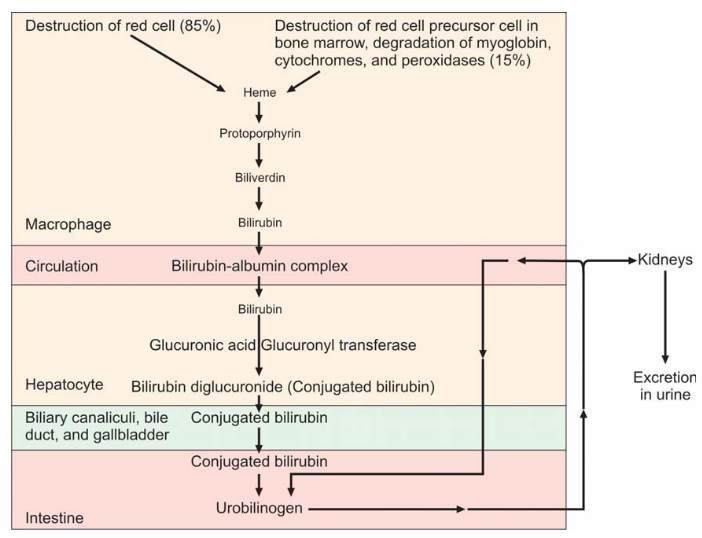
\includegraphics{image/bilirubin_normal.png}

}

\caption{Normal Bilirubin Metabolism}

\end{figure}%

\begin{enumerate}
\def\labelenumi{\arabic{enumi}.}
\item
  HB, degraded within macropahes to form heme and globin. Globin consist
  of amino acids, which are recycled. While Heme (iron + protoporphyrin)
  release iron, which is stored as ferritin. The protoporphyrin then
  converted to biliverdin, then to bilirubin.(Kawthalkar 2018)
\item
  Released bilirubin into the circulation and bind albumin, this called
  unconjugated bilirubin. It is insoluble to water, but lipid soluble.
\item
  Billirubin-albumin complex reaches the liver whee it is taken up by
  the hepatocytes. Albumin released back to the circulation.
\item
  Bilirubin then conjugated with glucoronic acid to form bilirubin
  monoglucoronid and diglucoronid (conjugated bilirubin). This Process
  is mediated by the ezyme glucoronyl transferase. Conjugated bilirubin
  is more soluble in water.
\item
  Conjugated bilirubin is secreted from the hepatocytes into biliary
  canaliculi, from where it passes into the bile duct and gallbladder
  along with bile.
\item
  When bilirubin reaches the large instensites, it is converted to
  urobilinogen by the baterial enzyme.
\item
  Most urobilinogen is excreted in feses as urobilin, thus coloring the
  feses yellow. A part of urobilinogen is absorbed into the circlation
  from where it reaches the liver, taken up and reexcreted into the
  bile. Small amaount of urobilinogen in cleared in urine.
\end{enumerate}

Jaundice or icterus referes to yellow discoloration of skin, screa and
mucous membranes due to increased level of serum bilirubin. Jaundice
will clinicaly evident when serum bilirubin level exceeds \textbf{2.0
mg/dL}.

\begin{enumerate}
\def\labelenumi{\arabic{enumi}.}
\tightlist
\item
  According to type of dominant bilirubin:
\end{enumerate}

A. Predominant unconjugated hyperbilirubinemia

If \textgreater{} 85\% of total is unconjugated bilirubin or indirect
bilirubin. The cause are hemolysis, ineffective eryhtropoeisus,
resorption large hematome, gilbert syndrome.

B. Predominant conjugated hyperbilirubinemia

If \textgreater{} 50\% of total is conjugated or direct bilirubin. Cause
are hepatitis, cirrhosis, cholestasis, drugs (anabolic steroid, oral
contraceptives), toxin, dubin johnson syndrome, rotor syndrome

C. Mixed (Conjugated and Unconjugated)

if conjugated bilirubin is 20-50\% of total, it may results from viral
or alcoholic hepatisis.

\begin{enumerate}
\def\labelenumi{\arabic{enumi}.}
\setcounter{enumi}{1}
\tightlist
\item
  According to site of disease
\end{enumerate}

\begin{figure}

{\centering 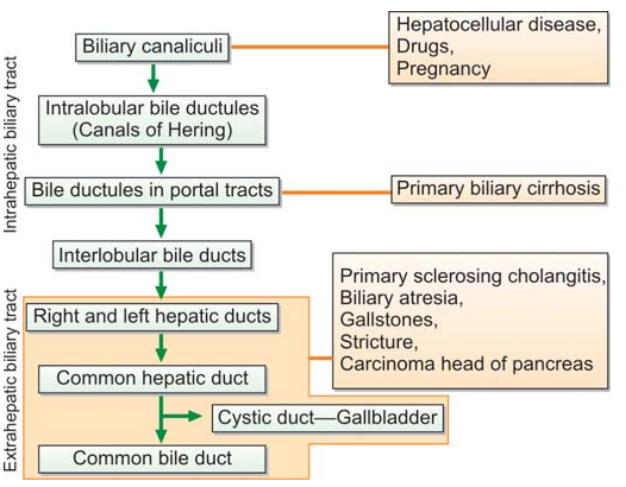
\includegraphics{image/Site_Cholestasis.png}

}

\caption{Sites of Cholestasis}

\end{figure}%

A. Prehepatic There is excessive formation of bilirubin exceeding the
capacity of the liver to conjugate it for excretion. The dominant
bilirubin is unconjugated. Bilirubin is absent in urine, since of is
water insoluble. Urobilinogen is increased in urine and feses. Jaudice
is usually mild (total bilirubin usually \textless{} 5.0 mg/dl,
conjugated is \textless{} 15\% of total). The cuase is usually
hematological problem.

B. Hepatic

Both Unconjugated and Conjuated are increased. mainly increased
unconjunjugated 1. defective uptake 2. defective conjugation 3.
physiologic jaundice (newborn)

mainly Conjugated ilirubin 1. Hepatocellular disease: Liver enzume
increase. Biliruibin is around 4.0 s.d 8.0 mg/dl. Conjugated bilirubin
is 20-50\% of total bilirubin. In hepatocellular injury, both conjugated
and unconjugated bilirubins are increased. Unconjugated bilirubin is
increased due to reduced ability of liver cells to conjugate bilirubin.
Conjugated bilirubin is raised from cholestasis due to hepatocyte
swelling.

\begin{enumerate}
\def\labelenumi{\arabic{enumi}.}
\setcounter{enumi}{1}
\tightlist
\item
  Intrahepatic Cholestasis: In intrahepatic cholestasis, there may be
  (1) impairment of secretion of bilirubin from hepatocytes into the
  biliary canaliculi; (2) obstruction of bile flow in canaliculi by
  swollen hepatocytes;or (3) damage to intrahepatic canaliculi.
\end{enumerate}

Drugs commonly associated with cholestatic injury are oral
contraceptives, anabolic steroids, oral anti-diabetics, phenothiazines,
and erythromycin.

Primary biliary cirrhosis, there is autoimmune destruction of
intrahepatic bile ducts. It predominantly occurs in middle-aged, females
and is characterized by chronic eleva- tion of alkaline phosphatase and
positive anti-mitochondrial antibody in serum.

Primary sclerosing cholangitis is an autoimmune disorder occurring in
young to middle-aged men in whom there is inflammation and destruction
of both intrahepatic and extra-hepatic bile ducts. Associated
inflammatory bowel disease is often present. Serum alkaline phosphatase
is elevated and many patients have circulating perinuclear
antineutrophil cytoplasmic antibodies.

C. Post Hepatic

Obstruction of extrahepatic biliary tract prevents flow of bile into the
duodenum. This causes ``regurgitation'' of conjugated bilirubin into the
circulation. (Biliary canaliculi distend and rupture due to backpressure
of bile and conjugated bilirubin escapes into the sinusoids). Conjugated
bilirubin is usually \textgreater50\% of total in posthepatic jaundice.
Urinary and fecal urobilinogen are decreased, faeces are clay-colored,
and bilirubin (being conjugated and water-soluble) appears in urine.
Cause of Posthepatic Jaundice:

\begin{itemize}
\tightlist
\item
  Carcinoma of head of pancreas
\item
  Carcinoma of ampulla of Vater
\item
  Secondaries in porta hepatis
\item
  Gallstones in or stricture of common bile duct
\end{itemize}

\begin{figure}

{\centering 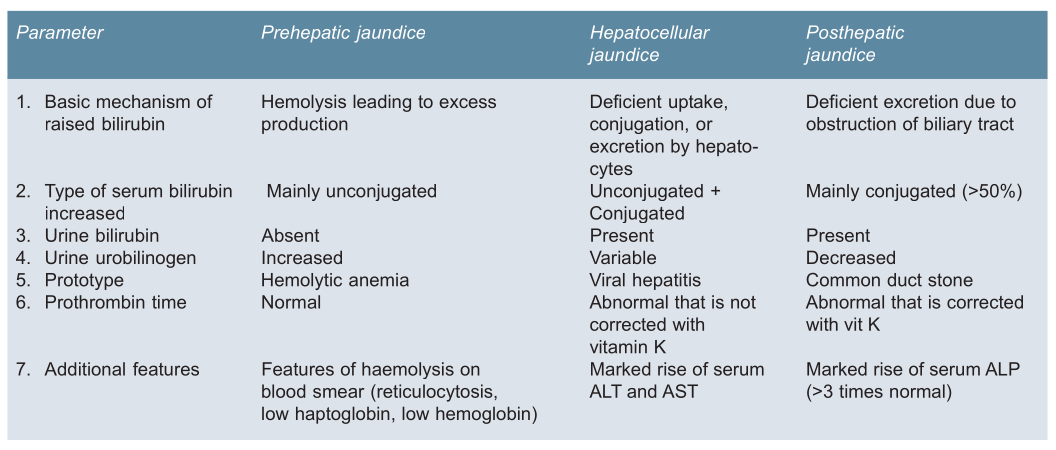
\includegraphics{image/Types_jaundice.png}

}

\caption{Three types of Jaundice Differential Diagnosis}

\end{figure}%

\subparagraph{Clinial Algorithm of
Jaundice}\label{clinial-algorithm-of-jaundice}

Normal serum bilirubin is less than 1 mg/dl. conjugated bilirubin is
10\% or less, while unconjugated bilirubin is 90\% or more. This is
because conjugated bilirubin is rapidly secreted into the bile after its
formation and removed through the gut. Conjugated bilirubin is composed
of blirubin glucuronide, bilirubin diglucuronide, and delta (δ)
bilirubin. Delta bilirubin represents bilirubin covalently bound to
albumin in circulation. Normally, δ bilirubin is absent or present in
very small amount. In cholestasis, proportion of δ-bilirubin increases.
Owing to its longer half-life, it is cleared slowly from circulation.
Conjugated bilirubin is weakly bound to albumin, is water-soluble, and
can be excreted in urine. Unconjugated bilirubin is tightly bound to
albumin and is water-insoluble.

\begin{figure}

{\centering 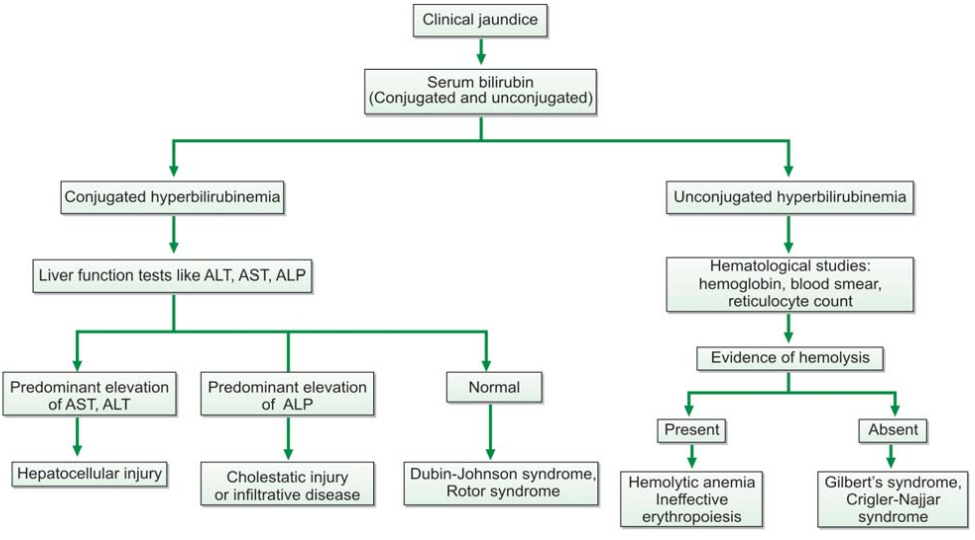
\includegraphics{image/jaundice_algorithm.png}

}

\caption{Jaundice Algorithm}

\end{figure}%

\paragraph{Synthetic Function}\label{synthetic-function}

Markers of hepatic synthetic function are serum albumin and prothrombin
time (PT). Hypoalbuminemia and a prolonged PT indicate a severe
functional impairment of liver.

\subparagraph{Protein Synthetic}\label{protein-synthetic}

Liver is the sole organ to synthesisze plasma protein, except gamma
globulin which synthesized by Plasma Cell. Normal total serum protein in
adults is about 5.5 - 8.0 gm / dl, albumin 3.5 - 5.0 which comprise the
60\% of serum protein.

Test for protein in liver disease incldue total serum protein, serum
albumin, calculation of albumin/globulin rtio (normal \textgreater{}
1.5) and serum electrophoresis.the common laboratory method to measure
total protein is biuret and refractometer method.

Total serum protein level is affected by both and gamma globulins. In
cirrhosis, decrease in albumin level is often compensated by increase in
the level of gamma globulins; therefore, estimation of total serum
proteins is of limited value in cirrhosis. Estimation of serum albumin
and serum protein electrophoresis are more helpful.

Albumin is synthesized exclusively in liver and constitutes about 60\%
of total proteins in serum; therefore its estimation is an important
investigation in liver disease. Half-life of albumin is about 20 days
and therefore fall in its level in response to decreased synthesis is
not immediately apparent. Therefore, in acute liver disease (e.g.~viral
hepatitis), there is little change in albumin level. Serum albumin level
is low in chronic liver disease (cirrhosis) and correlates with
synthetic capacity of hepatocytes; therefore, it is helpful in following
progression of cirrhosis. Also, fall in serum albumin level correlates
with severity of ascites. In cirrhosis and in chronic active hepatitis,
serum gamma globulins are increased due to inflammation. Low albumin and
raised gamma globulins in serum cause reversal of albumin/globulin
ratio. Serum albumin is estimated by bromocresol green method

Causes of decreased serum albumin: • Decreased intake: malnutrition. •
Decreased absorption: malabsorption syndromes. • Decreased synthesis:
liver disease, chronic infections. • Increased catabolism:
thyrotoxicosis, fever, malignancy, infections. • Increased loss:
nephrotic syndrome, severe burns, protein-losing enteropathies, ascites
• Increased blood volume: pregnancy, congestive cardiac failure.

Serum Protein Elektrophoresis: 1. In cirrhosis, albumin may be reduced
and there may be polyclonal increase of IgG and IgA, with β-γ bridging.
(IgA migrates between β and γ regions which obscures the demarcation
between β and γ peaks). 2. In primary biliary cirrhosis, there is
polyclonal increase of IgM. 3. In α1-antitrypsin deficiency (associated
with cirrhosis) α1- globulin band is reduced. 4. In chronic active
hepatitis, IgG is elevated.

\begin{figure}

{\centering 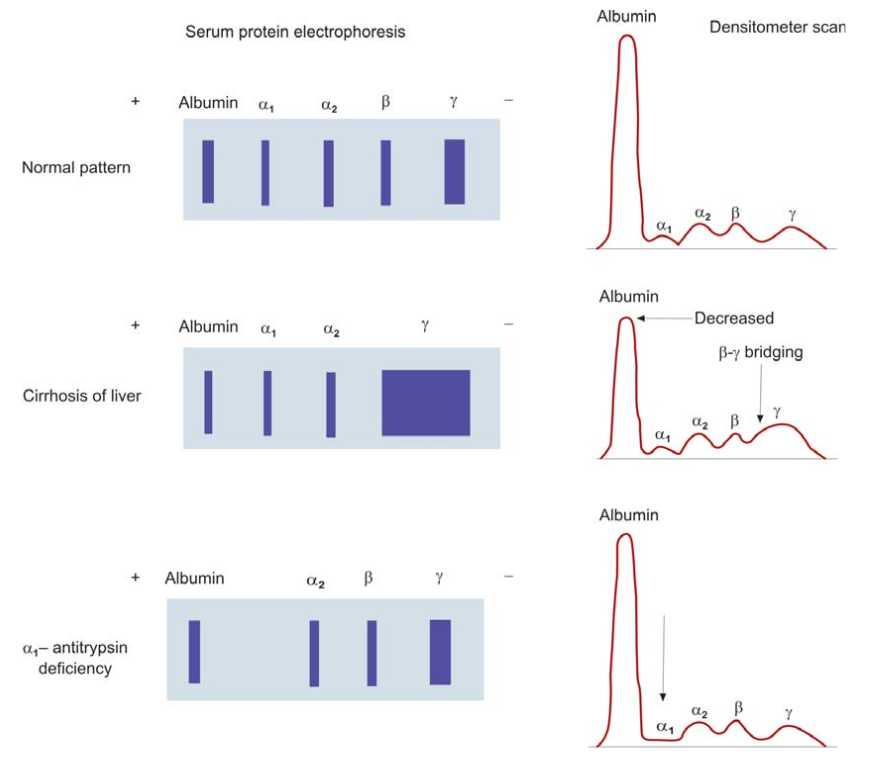
\includegraphics{image/spe.png}

}

\caption{Serum Protein Electrophoresis patterns and densitometer scans
in Normal, Cirhosis and Alpha 1 antitripsin deficienct individuals}

\end{figure}%

\subparagraph{Prothorombin Time (PT)}\label{prothorombin-time-pt}

Most of the coagulation protein are synthesized in the liver. Vitamin K
is required for the synthesis of factors II, VII, IX, X by the
hepatocytes, thus it is called vitamin K dependent factors. Synthesis of
the factors is deficient in hepatocellular disease. In Addition, in
obstructive jaundice, vitamin K (a fat soluble vitamin) cannot be
absorbed due to the absence of bile in the intentine.

PT measures three out of four vitamin K-dependent factors (II, VII, and
X) and is prolonged in hepatocellular disease and in obstructive
jaundice. Intramuscular injection of vitamin K corrects prolonged PT in
obstructive jaundice but not in hepatocellular jaundice. To distinguish
between a prolonged PT due to hepato- cellular disease from that due to
cholestasis with fat malabsorption, PT is repeated after administration
of vitamin K. Reduction of prolonged PT occurs in cholestatic liver
disease, but not in hepatocellular disease. In acute fulminant liver
failure, marked prolongation of PT is an unfavourable prognostic sign.

\subparagraph{Blood Ammonia}\label{blood-ammonia}

Blood ammonia is mainly derived from GI tract. In the gut, bacterial
enzyme act on nitrogen-containing foods to produce ammonia, which is
carried to the liver via portal vein. In the liver, ammonia is converted
to non -toxic urea in urea cycle.

Increased blood ammonia seen in: - Fulminant hepatic failure - cirrhosis
- Reye's Syndrome - ``Shunting'' of portal blood to systemic circulation
- Gastrointestinal hemmorhage (there is increased of production of
ammonia from blood proteins by bacterial enzymes). In hepatic disease,
gastrointestinal hemmorhage is associated with increased risk of hepatic
encepalopathy. - Inherited deficiensys of ure cycle enzymes.

If the ammonia is inreased, it might helful indicates a hepatic
encepalopathy.

\paragraph{Test Hepatocellular Injury}\label{test-hepatocellular-injury}

Serum enzyme changes in liver disease result from hepatocyte damage and
do not indicate hepatic functional capacity.

\begin{itemize}
\tightlist
\item
  Serum aspartate aminotransferase or AST (formerly called serum
  glutamic-oxaloacetic transaminase or SGOT)
\item
  Serum alanine aminotransferase or ALT (formerly called serum
  glutamic-pyruvic transaminase or SGPT)
\item
  Serum alkaline phosphatase or ALP
\item
  γ-Glutamyl transferase or GGT (also called as - γ-glutamyl
  transpeptidase)
\item
  5'-nucleotidase (5'-NT)
\end{itemize}

\subparagraph{Serum Aminotransferase
(Transaminitis)}\label{serum-aminotransferase-transaminitis}

Both AST and ALT are sensitive marker of hepatocellular injury. ALT is
cytosolic enzyme, AST is cytosolic and mitochondria. Normally,
aminotransferases are present in serum at a low level. When necrosis or
death of cells containing these enzymes occurs, aminotransferases are
released into the blood and their concentration in blood increases. This
level correlates with extent of tissue damage.

\textbf{``Most marked elevations of ALT and AST (\textgreater15 times
normal) are seen in acute viral hepatitis, toxin-induced hepatocellular
damage (e.g.~carbon tetrachloride), and centrilobular necrosis due to
ischemia (congestive cardiac failure).''}

Moderate elevation (5-15X normal) occurs due to chronic hepatitis,
autoimmune hepatitis, alcoholic hepatitis, acute biliary tract
obstruction, and drug induced hepatitis. Mild elevation (1-3 x normal)
seen in cirrhosis, non-alcoholic steatosis and cholestasis.

Normal ratio AST/ALT is 0.7 to 1.4. Increased ratio (\textgreater2.0) is
highly suggestive of alcoholic hepatitis, while ratio \textless1.0 is
seen in acute viral hepatitis. ALT and AST are elevated in acute viral
hepatitis even before the appearance of jaundice. Persistence of
elevated ALT and AST beyond 6 months in a case of hepatitis indicates
development of chronic hepatitis. Measurement of ALP is helpful in
differentiation of hepatocellular jaundice from cholestatic jaundice.

\subparagraph{Serum Alkaline Phospatase
(ALP)}\label{serum-alkaline-phospatase-alp}

Alkaline phosphatase is distributed widely in various tissues like
liver, bones, intestine, kidney, and placenta. In the liver, ALP, GGT,
and 5'-NT are located normally on canalicular surface of hepatocytes. In
cholestasis, accumulated bile acids dissolve canalicular side of
hepatocyte membrane and enzymes are released in blood. Therefore,
diseases that affect mainly hepatocyte secretion have elevated levels of
ALP.

ALP is increased in most cases of cholestatic type of jaundice. While
hepatocellular injury is characterized by marked elevation of ALT and
AST, cholestasis is characterized by marked increase (more than 3 times
normal) of ALP. Since there are many other sources of ALP apart from
liver, simultaneous measurement of serum GGT and serum 5'-NT may be used
to ascertain whether increase of ALP is of hepatic origin. Main cause of
increased ALP due to hepatobiliary disease are: Bile duct obstruction,
primary biliarry cirhosis, primary sclerosing cholangitis, infilstrative
diseae of liver.

Disease of bones also could cause increased ALP. ALP present within
osteoblasts, thus ALP increase when there is an increase osteoblastic
activity. Pregnancy also increase ALP due to increased secretion from
plancenta.

\subparagraph{Serum Gamma-Glutamyl Transferase
(GGT)}\label{serum-gamma-glutamyl-transferase-ggt}

GGT presents in liver, pancreas, kidney, and prostate. The estimation of
this enzyme is particularly useful in following: alcoholism (acute
alcoholic hepatitis); Cholestasis (elevation of ALP and GGT
significantly points toward liver disease); recovery from acute
hepatitis (GGT is the last enzyme to return to normal, thus its
normalization indicative favourable outcome)

\subsubsection{Interpretation of Liver Function
Test}\label{interpretation-of-liver-function-test}

Liver disease could broadly classified into two: hepatocellular and
cholestasis.

\textbf{1. Typical LFT profile in hepatocellular disease}

• Marked elevation of AST and ALT (usually \textgreater500 IU)

• Mild increase of ALP (\textless3 times normal)

• Hyperbilirubinemia, if present, is of both conjugated and unconjugated
type

• Chronic hepatocellular injury, aminotransferases are moderately
elevated, and serum albumin is reduced.

If the LFT showed a hepatocellular disease, then next investigation is
to detect underlying cause:

\begin{itemize}
\tightlist
\item
  Viral serology (viral hepatitis: IgM anti-hepatitis A antibody,
  hepatitis surface B antigen (HBsAg), antihepatitis C antibody),
\item
  search for injurious drugs, toxins or alcohol,
\item
  autoantibodies like antinuclear antibodies and anti-smooth muscle
  antibodies (autoimmune hepatitis), and serum ceruloplasmin (Wilson
  disease).
\end{itemize}

\begin{figure}

{\centering 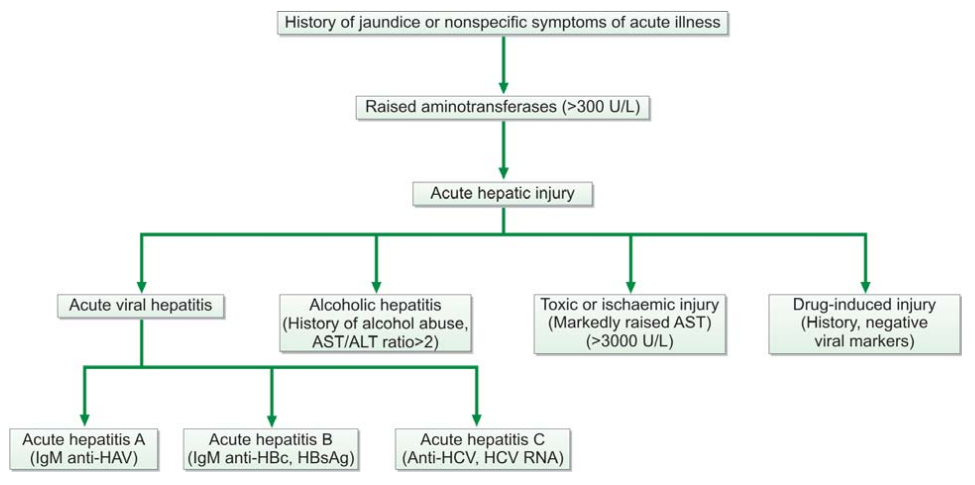
\includegraphics{image/hepatocellular_injury.png}

}

\caption{History of Jaundice of nonspecific acute illness in the setting
of increased aminotransferase}

\end{figure}%

If cause is not detected in the presence of persistent elevation of
aminotransferases, liver biopsy is performed (that may reveal chronic
viral hepatitis, autoimmune disorders, Wilson disease, haemochromatosis,
and infiltrative diseases)

\textbf{2. Typical LFT profile in cholestatic jaundice}

• Marked elevation of ALP (\textgreater3 times normal)

• Elevation of GGT and 5'-NT

• Mild or no increase of ALT and AST (usually \textless200 IU)

• Elevation of conjugated bilirubin

• The pattern of elevated ALP but normal serum bilirubin is seen in
infiltrative diseases

\begin{figure}

{\centering 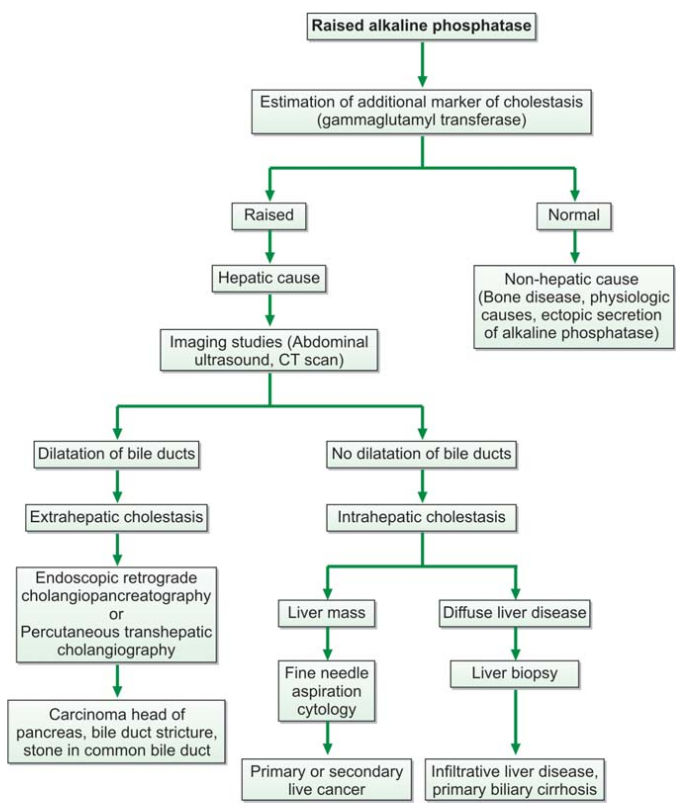
\includegraphics{image/cholestatic_injury.png}

}

\caption{Evaluation of Raised ALP in the suspicion of cholestatic
injury}

\end{figure}%

In patients with cholestatic or infiltrative pattern of injury, imaging
studies should be done for diagnosis of obstruction. If there is no
evidence of obstruction, liver biopsy is usually done

Finally, Severity of liver disease is assessed by serum bilirubin, serum
albumin, and prothrombin time. Child-Turcotte-Pugh classification is
commonly used to assess severity of cirrhosis and is based on both
clinical and laboratory parameters

\begin{figure}

{\centering 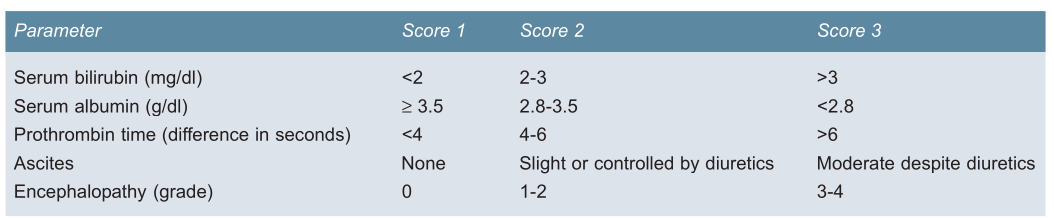
\includegraphics{image/CTP.png}

}

\caption{Child-Turcotte-Pugh score to assese severity of cirhosis}

\end{figure}%

\paragraph{Normal Values}\label{normal-values}

Serum alanine aminotransferase (ALT, SGPT): 5-42 U/L

Serum aspartate aminotransferase (AST, SGOT): 5-40 U/L

Serum alkaline phosphatase (ALP):

• Children: 25-350 U/L

• Adult males: 25-120 U/L

• Adult females: 25-90 U/L

AST/ALT ratio: 0.7-1.4

Serum bilirubin:

• Total: 0.3-1.0 mg/dl

• Direct (Conjugated): 0-0.2 mg/dl

Serum proteins, total: 5.5-8.0 gm/dl

Serum albumin: 3.5-5.0 gm/dl

Serum globulins: 1.8-3.5 gm/dl

Albumin/Globulin (A/G) ratio: \textgreater1.5

Prothrombin time: 11-15 seconds

Plasma ammonia: 9-33 μmol/L

Serum gammaglutamyl transferase:

• Males: Up to 40 U/L

• Females: Up to 25 U/L

Serum protein electrophoresis:

Albumin 52-65\%

α1 globulin: 2.5-5\%

α2 globulin: 7-13\%

β globulin: 8-14\%

γ globulin: 12-22\%

\subsection{Disorder of Lipids}\label{disorder-of-lipids}

\subsection{Cardiac markers}\label{cardiac-markers}

\subsection{Coagulation Study}\label{coagulation-study}

\subsection{Renal Function Test}\label{renal-function-test}

Kidney performs following functions: 1. maintenance of extracellular
fluid volume \& composition 2. Excretion of metabolic waste 3.
Regulation of blood pressure 4. synthesis of erytheropoeitin 5.
Production of Vitamin D3

Kidney functions affected by:

\begin{enumerate}
\def\labelenumi{\arabic{enumi}.}
\tightlist
\item
  Diffuse renal disease
\item
  Pre-renal conditions
\item
  Post-renal conditions
\end{enumerate}

\textbf{Classification of renal Function Test}

A. Evaluation of Glomerular Function

B Evaluation of Tubular Function

\subsubsection{A. Test to Evaluaste Glomerular
Function}\label{a.-test-to-evaluaste-glomerular-function}

The best test to evaluate overall kidney functions is estimation of GFR.
GFR varies with age, sex and BSA. Normal GFR in young adults is 120-130
ml/min per 1.73 m2 of body surface area. GFR declines progressively with
age (due to arteriolosclerosis of glomeruli). After 40 years of age,
there is a steady and progressive fall in the GFR at the rate of 1
ml/minute/year because of reduction in the number of glomeruli due to
arteriolosclerosis.

Kdigo 2022 divide Chronic Kidney Disease into :

\begin{enumerate}
\def\labelenumi{\arabic{enumi}.}
\item
  Stage 1; Kidney damage with Normal to increased GFR (GFR \(\geq\) 90
  ml / min / 1.73 m\textsuperscript{2})
\item
  Stage 2; Kidney damage with Mildly reduced GFR (GFR 60 - 89 ml / min /
  1.73 m\textsuperscript{2})
\item
  Stage 3; Moderately reduced GFR (GFR 30 - 59 ml / min / 1.73
  m\textsuperscript{2})
\item
  Stage 4; Severely reduced GFR (GFR 15 - 29 ml / min / 1.73
  m\textsuperscript{2})
\item
  Stage 5; Kidney Failure (GFR \(\leq\) 15 ml / min / 1.73
  m\textsuperscript{2})
\end{enumerate}

Kidney damage refers to presence of pathological abnormalities in blood
or urine test or imaging studies. Symtoms usually present at GFR less
than 60, which reflect loss of 50\% Kidney Function.

GFR, glomerular filtration rate referes to the rate in ML/min at which a
substance is cleared from the circulation by the glomeruli. The ability
of the glomeruli to filter a substance from the blood is assessed by
clearance studies. If a substance is not bound to protein in plasma, is
completely filtered by the glomeruli, and is neither secreted nor
reabsorbed by the tubules, then its clearance rate is equal to the
glomerular filtration rate (GFR).

Clearance of a substance refers to the volume of plasma, which is
completely cleared of that substance per minute; it is calculated from
the following formula:

\[
clearance = \frac{UV}{P}
\]

U: concentration of substance in urine (mg/dl)

V: volume of urine excreted in ml/min

P: concentration of substance in plasma (mg/dl)

all clearance value are adjusted to standard body surface area: 1.73
m\textsuperscript{2}.

Clearance tests are cumbersome to perform, expensive, and not readily
available. One major problem with clearance studies is incomplete urine
collection.

The Particular ``substance'' are molecules which having the following
properties: 1. It should be physiologically inert and preferably
endogenous,

\begin{enumerate}
\def\labelenumi{\arabic{enumi}.}
\setcounter{enumi}{1}
\tightlist
\item
  It should be freely filtered by glomeruli and should be neither
  reabsorbed nor secreted by renal tubules,
\end{enumerate}

3 It should not bind to plasma proteins and should not be metabolized by
kidneys

4 It should be excreted only by the kidneys

Example of substance used to measure GFR are:

\begin{enumerate}
\def\labelenumi{\arabic{enumi}.}
\item
  Exogenous: Inulin, Radiolabelled ethylenediamine tetraacetic acid
  (51Cr- EDTA), 125I-iothalamate
\item
  Endogenous: Creatinine, Urea, Cystatin C
\end{enumerate}

\paragraph{Inulin Clearance}\label{inulin-clearance}

Inulin is inert polysacharide derived from the plant. It is called inert
as it is freely filtered by the glomerulus, and is neither reabsorbed
nor secreted by the tubules thus Inulin is an ideal agent for measuring
GFR.

Protocol: A bolus dose of inulin (25 ml of 10\% solution IV) is
administered followed by constant intravenous infusion (500 ml of 1.5\%
solution at the rate of 4 ml/min). Timed urine samples are collected and
blood samples are obtained at the midpoint of timed urine collection.
Average inulin clearance for males is 125 ml/min/1.73 m2 and for females
is 110 ml/min/1.73 m2.

\paragraph{Cystatin C Clearance}\label{cystatin-c-clearance}

This is a cysteine protease inhibitor of MW 13,000, which is produced at
a constant rate by all the nucleated cells. It is not bound to protein,
is freely filtered by glomeruli and is not returned to circulation after
filtration. It is a more sensitive and specific marker of impaired renal
function than plasma creatinine. Its level is not affected by sex, diet,
or muscle mass. It is thought that cystatin C is a superior marker for
estimation of GFR than creatinine clearance.

\paragraph{Creatinine Clearance}\label{creatinine-clearance}

Creatinine is being produced constantly from creatine in muscle. It is
completely filtered by glomeruli and is not reabsorbed by tubules;
however, a small amount is secreted by tubules.

A 24-hour urine sample is preferred. After getting up in the morning,
the first voided urine is discarded. Subsequently all the urine passed
is collected in the container provided. After getting up in the next
morning, the first voided urine is also collected and the container is
sent to the laboratory.

A blood sample for estimation of plasma creatinine is obtained at
midpoint of urine collection.

Creatinine clearance is calculated from:

\begin{enumerate}
\def\labelenumi{\arabic{enumi}.}
\item
  concentration of creatinine in urine in mg/ml (U),
\item
  volume of urine excreted in ml/min (V) (this is calculated by the
  formula: volume of urine collected/collection time in minutes
  e.g.~volume of urine collected in 24 hours ÷ 1440)
\item
  concentration of creatinine in plasma in mg/dl (P).
\item
  Creatinine clearance in ml/min per 1.73 m2 is then derived from the
  formula UV/P.
\end{enumerate}

Because of secretion of creatinine by renal tubules, the above formula
overestimates GFR by about 10\%. In advanced renal failure, secretion of
creatinine by tubules is increased and thus overestimation of GFR is
even more. Overestimation of GFR due to tubular secretion of creatinine
is somewhat balanced by slight overestimation of serum creatinine by
Jaffe's reaction. To provide values closer to the actual GFR, cimetidine
(which blocks secretion by renal tubules) can be administered before
commencing urine collection

Creatinine clearance has few weakness:

\begin{enumerate}
\def\labelenumi{\arabic{enumi}.}
\item
  Tubular secretion of creatinin that icrease as the kidney disease
  advance
\item
  Collection of urine often incomplete
\item
  Creatinin level is affected by protein intake and muscle mass
\item
  Creatinine level also affected by drugs, ie Cimetidine, Trimetophrim
  (which block tubular secretion of creatinine)
\end{enumerate}

Tips: BUN and serum creatinine, by themselves, are not sensitive
indicators of early renal impairment since values may be normal e.g.~if
baseline values of serum creatinine is 0.5 mg/dl, then 50\% reduction in
kidney function would increase it to 1.0 mg/dl. Thus clearance tests are
more helpful in early cases. If biochemical tests are normal and renal
function impairment is suspected, then creatinine clearance test should
be carried out. If biochemical tests are abnormal, then clearance tests
need not be done.

\paragraph{Urea Clearance}\label{urea-clearance}

Urea is filtered by the glomeruli, but about 40\% of the filtered amount
is reabsorbed by the tubules. The reabsorption depends on the rate of
urine flow. Thus it underestimates GFR, depends on the urine flow rate,
and is not a sensitive indicator of GFR.

\paragraph{Estimation of Creatinine Clearance from serum creatinin by
equation}\label{estimation-of-creatinine-clearance-from-serum-creatinin-by-equation}

Estimation of GFR from Serum creatinin depend on age, sex, body weight
and serum creatinine value (and in some formula includes ethnicity).
This is called as estimated GFR (eGFR).

\begin{enumerate}
\def\labelenumi{\arabic{enumi}.}
\tightlist
\item
  Modified Cockroft Gauld Equation (if SC Mg/Dl) \[
  Creatine Clearance (ml/min) = \frac{(140 - age) \times (Weight) }{72 \times SC} 
  \]
\end{enumerate}

In females, the value obtained from above equation is multiplied by 0.85
to get the result.

\begin{enumerate}
\def\labelenumi{\arabic{enumi}.}
\setcounter{enumi}{1}
\item
  Modification of Diet in Renal Disease (MDRD) equation for estimated
  eGFR: \[
  eGFR (mL/min/1.73 m2) = 175 × (s. creatinine in mg/dL) – 1.154 × (Age in year)–0.203 × (0.742 if female) × (1.210 if African – American)
  \] This is applicable for adults between 18 and 70 years of age. It is
  more accurate than measured creatinine clearance from 24-hour urine
  collection and Cockroft-Gault equation. This is the most commonly used
  equation.
\item
  CKD-EPI (chronic kidney disease-epidemiology) equation: This is a
  recently introduced more accurate equation.
\end{enumerate}

\[
eGFR (mL/min/1.73 m2) = 141 × min (Scr/k,1)a × max (Scr/k, 1)–1.209 × (0.993)Age ×
1.018 (if female) × 1.159 (if black)
\] where, Scr = Standardized serum creatinine (mg/dL) K = 0.7 (female)
or 0.9 (male) a = --0.329 (female) or --0.411 (male), min = minimum of
Scr/k or 1, max = maximum of Scr/k or 1, Age = years

\begin{enumerate}
\def\labelenumi{\arabic{enumi}.}
\setcounter{enumi}{3}
\tightlist
\item
  In Children, Schwartz formula is used for estimation of GFR:
\end{enumerate}

\[
Estimated GFR = \frac{K \times Height (cm)}{Sc}
\] k = 0.33 in preterm babies for the first year of life; k=0.45 for
full term infants; for infants and children up to 12 years of age k is
0.55.

Disadvantages of estimated GFR: 1. GFR estimated by Ckockcroft-Gault and
MDRD formulas tends to underestimate renal function at high levels of
GFR (\textgreater60 mL/minute/1.73 m2);

\begin{enumerate}
\def\labelenumi{\arabic{enumi}.}
\setcounter{enumi}{1}
\tightlist
\item
  Values may be misleading in acute kidney injury, pregnancy, decreased
  muscle mass (e.g.~paraplegia, muscle wasting disorders, critically
  ill, patients with cancer), increased muscle mass in athletes and body
  builders, unusual diets, and extremes of age or weight.
\end{enumerate}

\subparagraph{Blood Urea Nitrogen}\label{blood-urea-nitrogen}

Urea is produced in the liver from amino acids. Amino acids are utilized
to produce energy, synthesize proteins, and are catabolized to ammonia.
Urea is produced in the liver from ammonia in the Krebs urea cycle.
Ammonia is toxic, and hence, is converted to urea, which is then
excreted in urine.

The concentration of blood urea is usually expressed as blood urea
nitrogen. This is because older methods estimated only the nitrogen in
urea. Molecular weight of urea is 60, and 28 g of nitrogen are present
in a gram mole of urea. As the relationship between urea and BUN is
60/28, BUN can be converted to urea by multiplying BUN by 2.14, i.e.~the
real concentration of urea is BUN × (60/28). Urea is completely filtered
by the glomeruli, and about 30--40\% of the filtered amount is passively
reabsorbed in the renal tubules depending on the person's state of
hydration.

lood level of urea is affected by a number of nonrenal factors
(e.g.~dehydration, hypoperfusion of kidneys, high protein diet, protein
catabolism, upper gastrointestinal hemorrhage, liver function, steroid
administration, etc.), and therefore, utility of BUN as an indicator of
renal function is limited. Also considerable destruction of renal
parenchyma is required before elevation of blood urea can occur.

The term azotemia refers to the increase in the blood level of urea;
uremia is the clinical syndrome resulting from this increase. Reference
range for BUN in adults is 7--18 mg/dL. In adults \textgreater60 years,
level is 8--21 mg/dL. laboratory method to analyze BUN are Diacetyl
monoxime urea and urease-Brthol reaction.

\subparagraph{Serum Creatinin}\label{serum-creatinin}

Creatinine is a nitrogenous waste product formed in muscle from creatine
phosphate. Endogenous production of creatinine is proportional to muscle
mass and body weight. Exogenous creatinine (from ingestion of meat) has
little effect on daily creatinine excretion.

Serum creatinine is a more specific and more sensitive indicator of
renal function as compared to BUN because: - It is produced from muscles
at a constant rate and its level in blood is not affected by diet,
protein catabolism, or other exogenous factors - It is not reabsorbed,
and very little is secreted by tubules.

Significant kidney reserve, increase of serum creatinine level (from 1.0
mg/dl to 2.0 mg/dl) in blood does not occur until about 50\% of kidney
function is lost. Therefore, serum creatinine is not a sensitive
indicator of early renal impairment (\textbf{SC\_gfr?}). Laboratory
report showing serum creatinine ``within normal range'' does not
necessarily mean that the level is normal; the level should be
correlated with body weight, age and sex of the individual. If renal
function is absent, serum creatinine rises by 1.0 to 1.5 mg/dL/day.

\begin{figure}

{\centering 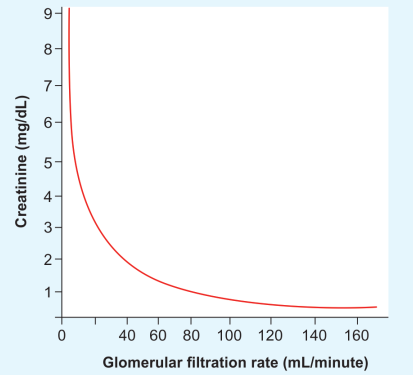
\includegraphics{image/SC-GFR.png}

}

\caption{Relationship between glomerular filtration rate and serum
creatinine. Significant increase of serum creatinine does not occur till
a considerable fall in GFR}

\end{figure}%

Causes of decreased serum creatinine level:

\begin{enumerate}
\def\labelenumi{\arabic{enumi}.}
\item
  Female sex.
\item
  Vegetarian diet.
\item
  Malnutrition, muscle wasting.
\item
  Increasing age (reduction in muscle mass)
\end{enumerate}

Methods to estimate serum creatinin is Jaffe reaction and Enzymatic
Methods. Reference range Adult males: 0.7--1.3 mg/dL. Adult females:
0.6--1.1 mg/dL.

\subparagraph{BUN/Serum Creatinin Ratio}\label{bunserum-creatinin-ratio}

BUN/creatinine ratio to discriminate prerenal and postrenal azotemia
from renal azotemia. Normal ratio is 12:1 to 20:1.

\textbf{Causes of increased BUN/creatinine ratio (\textgreater20:1):} 1.
Increased BUN with normal serum creatinine:

\begin{itemize}
\tightlist
\item
  Pre-renal azotemia (reduced renal perfusion)
\end{itemize}

-- High protein diet

-- Increased protein catabolism

-- Gastrointestinal hemorrhage.

\begin{enumerate}
\def\labelenumi{\arabic{enumi}.}
\setcounter{enumi}{1}
\tightlist
\item
  Increase of both BUN and serum creatinine with disproportionately
  greater increase of BUN:
\end{enumerate}

Postrenal azotemia (Obstruction to the outflow of urine) Obstruction to
the urine outflow causes diffusion of urinary urea back into the blood
from tubules because of backpressure.

\begin{enumerate}
\def\labelenumi{\arabic{enumi}.}
\setcounter{enumi}{2}
\tightlist
\item
  Causes of decreased BUN/creatinine ratio (\textless10:1):
\end{enumerate}

\begin{itemize}
\tightlist
\item
  Acute tubular necrosis
\item
  Low protein diet, starvation
\item
  Severe liver disease.
\end{itemize}

\subsubsection{B. Test To Evaluaste Tubular
Functions}\label{b.-test-to-evaluaste-tubular-functions}

Renal tubules efficiently reabsorb 99\% of the glomerular filtrate to
conserve the essential substances. Abnormality tubular function
includes:

\begin{enumerate}
\def\labelenumi{\arabic{enumi}.}
\item
  GLycosuria
\item
  Generalized Aminoaciduria
\item
  TUbular Proteinuria
\item
  Urinary concentration of sodium
\item
  Fractional excretion of sodum.
\end{enumerate}

\subsection{Urine Analysis}\label{urine-analysis}

\subsubsection{Macroscopy}\label{macroscopy}

\subsubsection{Microscopy}\label{microscopy}

\subsubsection{Chemical}\label{chemical}

\paragraph{Albuminuria}\label{albuminuria}

Normally, a very small amount of albumin is excreted in urine. The
earliest evidence of glomerular damage in diabetes mellitus is
occurrence of microalbuminuria (albuminuria in the range of 30 to 300
mg/24 hours). An albuminuria \textgreater300 mg/24 hour is termed
clinical or overt and indicates significant glomerular damage. Urine
protein to creatinine ratio on a randome urine sample has been shown to
correlate well with estimation of 24-hour urine protein.

\chapter{Clinical Microbiology}\label{clinical-microbiology}

\chapter{Ear, Nose \& Throat}\label{ear-nose-throat}

\chapter{Ophtalmology}\label{ophtalmology}

\chapter{Rehabilitation \& Physical
Medicine}\label{rehabilitation-physical-medicine}

\chapter{Disaster Medicine, Wilderness medicine, Transport
Medicine}\label{disaster-medicine-wilderness-medicine-transport-medicine}

\bookmarksetup{startatroot}

\chapter{Pharmacology}\label{pharmacology}

\bookmarksetup{startatroot}

\chapter{Common Medical Procedures for
Internist}\label{common-medical-procedures-for-internist}

\section{Diagnostics}\label{diagnostics}

\section{Therapeutics}\label{therapeutics}

\subsection{Blood Transfusion}\label{blood-transfusion}

\part{Bioinformatics \& Genomic Medicine}

\chapter{Genomic Medicine}\label{genomic-medicine}

\chapter{Linux \& Bioinformatic
Programs}\label{linux-bioinformatic-programs}

\part{Statistics and R languange}

\section*{Dataframe Operation}\label{dataframe-operation}
\addcontentsline{toc}{section}{Dataframe Operation}

\markright{Dataframe Operation}

Checking the columns

\begin{verbatim}
[1] "Field.Name"   "Area"         "Slope"        "Vegetation"   "Soil.pH"     
[6] "Damp"         "Worm.density"
\end{verbatim}

SUmmary

\begin{verbatim}
  Field.Name             Area           Slope        Vegetation       
 Length:20          Min.   :0.800   Min.   : 0.00   Length:20         
 Class :character   1st Qu.:2.175   1st Qu.: 0.75   Class :character  
 Mode  :character   Median :3.000   Median : 2.00   Mode  :character  
                    Mean   :2.990   Mean   : 3.50                     
                    3rd Qu.:3.725   3rd Qu.: 5.25                     
                    Max.   :5.100   Max.   :11.00                     
    Soil.pH         Damp          Worm.density 
 Min.   :3.500   Mode :logical   Min.   :0.00  
 1st Qu.:4.100   FALSE:14        1st Qu.:2.00  
 Median :4.600   TRUE :6         Median :4.00  
 Mean   :4.555                   Mean   :4.35  
 3rd Qu.:5.000                   3rd Qu.:6.25  
 Max.   :5.700                   Max.   :9.00  
\end{verbatim}

The use of aggregates function

\begin{verbatim}
   Arable Grassland    Meadow   Orchard     Scrub 
 5.333333  2.444444  6.333333  9.000000  5.250000 
\end{verbatim}

\begin{verbatim}
  Community     Area    Slope  Soil.pH Worm.density
1    Arable 3.866667 1.333333 4.833333     5.333333
2 Grassland 2.911111 3.666667 4.100000     2.444444
3    Meadow 3.466667 1.666667 4.933333     6.333333
4   Orchard 1.900000 0.000000 5.700000     9.000000
5     Scrub 2.425000 7.000000 4.800000     5.250000
\end{verbatim}

Multiple classification

\begin{verbatim}
  moisture community     Area    Slope  Soil.pH Worm.density
1    FALSE    Arable 3.866667 1.333333 4.833333     5.333333
2    FALSE Grassland 3.087500 3.625000 3.987500     1.875000
3     TRUE Grassland 1.500000 4.000000 5.000000     7.000000
4     TRUE    Meadow 3.466667 1.666667 4.933333     6.333333
5    FALSE   Orchard 1.900000 0.000000 5.700000     9.000000
6    FALSE     Scrub 3.350000 5.000000 4.700000     7.000000
7     TRUE     Scrub 1.500000 9.000000 4.900000     3.500000
\end{verbatim}

\subsubsection*{Get to Know the Data}\label{get-to-know-the-data}
\addcontentsline{toc}{subsubsection}{Get to Know the Data}

\paragraph*{Check if any unusual data
points}\label{check-if-any-unusual-data-points}
\addcontentsline{toc}{paragraph}{Check if any unusual data points}

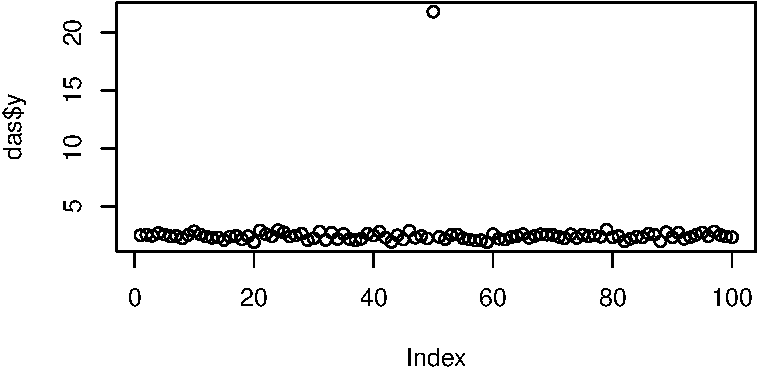
\includegraphics{statistics_files/figure-pdf/unnamed-chunk-7-1.pdf}

To find which data is the outlier in the above scatter plot

\begin{verbatim}
[1] 50
\end{verbatim}

So it is the the 50 th data point.

\paragraph*{Find Relathionsip}\label{find-relathionsip}
\addcontentsline{toc}{paragraph}{Find Relathionsip}

\subparagraph*{Numeric vs Numeric
Variabales}\label{numeric-vs-numeric-variabales}
\addcontentsline{toc}{subparagraph}{Numeric vs Numeric Variabales}

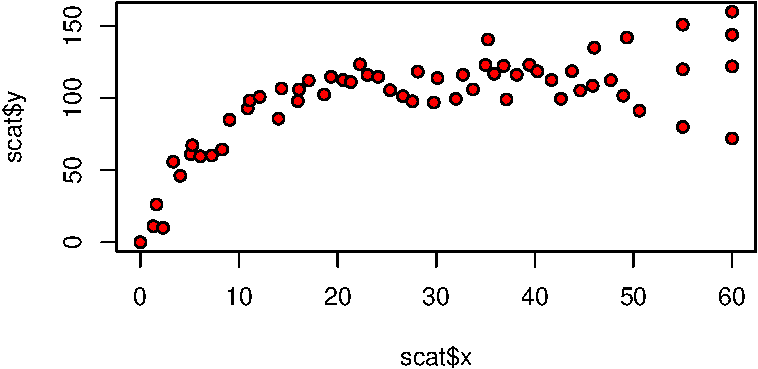
\includegraphics{statistics_files/figure-pdf/unnamed-chunk-9-1.pdf}

From plot above we can see : 1. The relathioship between response and
explanatory variables is curved 2. Degree of scatter from left to right
increases (non heterogenous), thus heterocedascity.

\subparagraph*{Categorical vs Numeric
Variabales}\label{categorical-vs-numeric-variabales}
\addcontentsline{toc}{subparagraph}{Categorical vs Numeric Variabales}

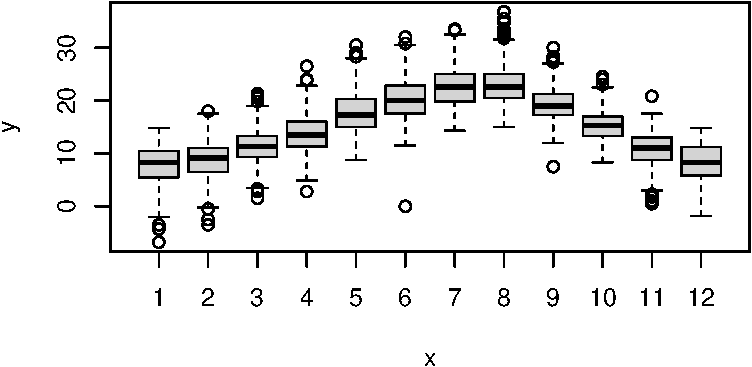
\includegraphics{statistics_files/figure-pdf/unnamed-chunk-10-1.pdf}

We see an overall pattern of temperature in a year. We see an outlier at
month-6, it turns out a missing data that inputted as zero.

\subparagraph*{making Conditional Plot
(COPLOT)}\label{making-conditional-plot-coplot}
\addcontentsline{toc}{subparagraph}{making Conditional Plot (COPLOT)}

Alter graphics parameter to specifiy two sets of axis on the same row
then make a simple scatter plot

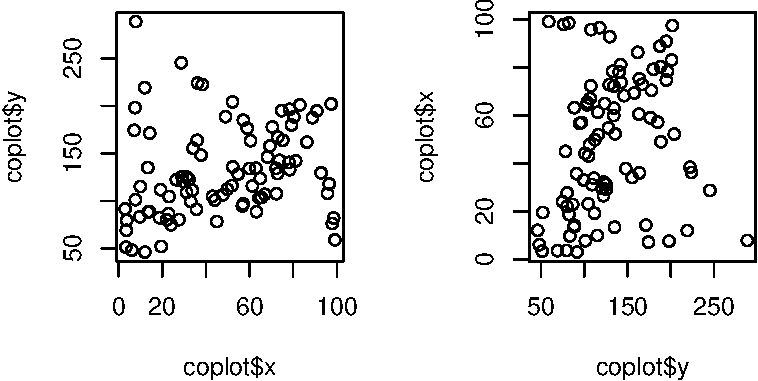
\includegraphics{statistics_files/figure-pdf/unnamed-chunk-12-1.pdf}

To look for interaction between explanatory variables and response
variables, we employ coplot. It plot Y agains X conditional on the value
of Z. Z is numeric variables, by default the coplot split Z into six
graphs, with the lowest value appear in the bottom left-hand.

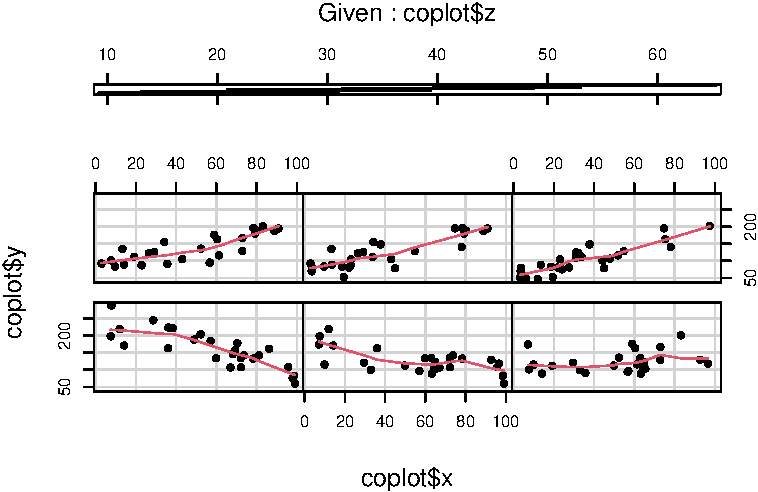
\includegraphics{statistics_files/figure-pdf/unnamed-chunk-13-1.pdf}

The relathiosip of X and Y change according to Z, as increasing Z the
trend comes positive.

\subparagraph*{Interaction in Categorical
Data}\label{interaction-in-categorical-data}
\addcontentsline{toc}{subparagraph}{Interaction in Categorical Data}

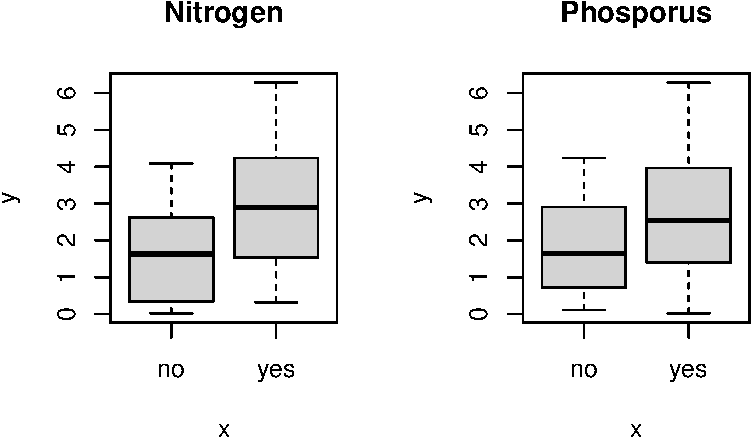
\includegraphics{statistics_files/figure-pdf/unnamed-chunk-15-1.pdf}

Finding mean for each groups

\begin{verbatim}
         no      yes
no  1.47384 1.875928
yes 2.28999 3.480184
\end{verbatim}

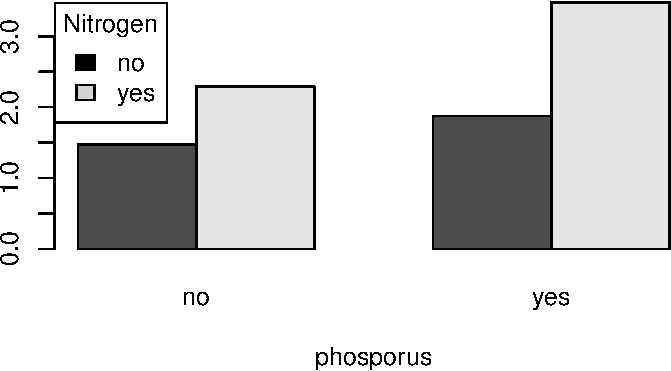
\includegraphics{statistics_files/figure-pdf/unnamed-chunk-17-1.pdf}

Nitrogen only, gives (effect sizes) 2.29/1.47 (1.55) while nitrogen +
phosporus gives 3,48/1.87 (1.86) increase in yield. Thus effect size of
nitrogen increase depends on phosporus. This is called statistical
interaction.

\section*{Central Tendency}\label{central-tendency}
\addcontentsline{toc}{section}{Central Tendency}

\markright{Central Tendency}

\section*{Variance}\label{variance}
\addcontentsline{toc}{section}{Variance}

\markright{Variance}

A measure of variability is perhaps the most important quantity in
statistical analysis. The greater variability \textasciitilde{} the
greater the uncertainty, the harder to distinguish competing hypothesis.

\subsubsection*{Ilustration of Variance}\label{ilustration-of-variance}
\addcontentsline{toc}{subsubsection}{Ilustration of Variance}

Just learn how to make the graph

Finding Range

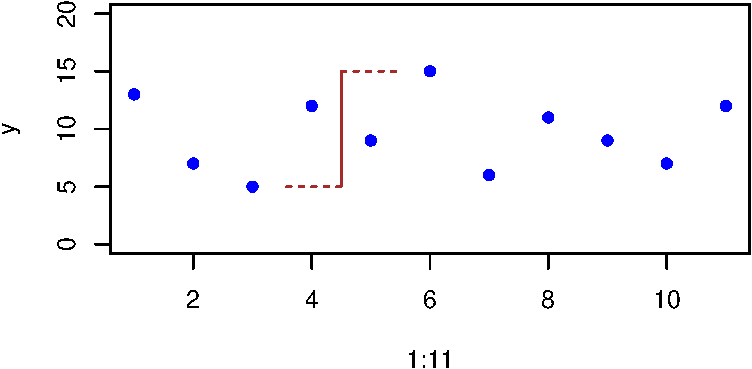
\includegraphics{statistics_files/figure-pdf/unnamed-chunk-18-1.pdf}

\begin{verbatim}
[1]  5 15
\end{verbatim}

\subsubsection*{Illustration of Mean
Value}\label{illustration-of-mean-value}
\addcontentsline{toc}{subsubsection}{Illustration of Mean Value}

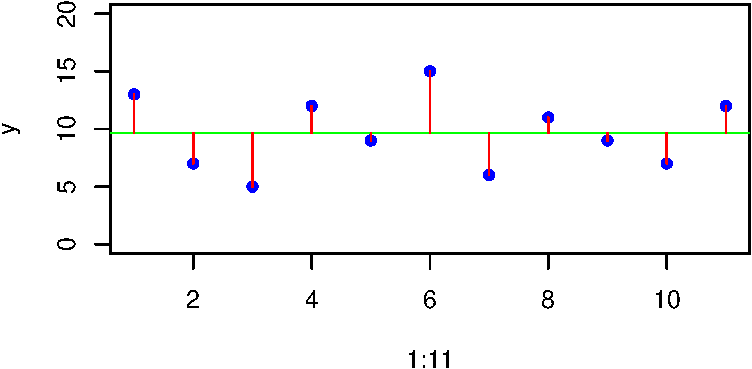
\includegraphics{statistics_files/figure-pdf/unnamed-chunk-19-1.pdf}

When Variance are different, dont compare the means.

\section*{Single-Samples}\label{single-samples}
\addcontentsline{toc}{section}{Single-Samples}

\markright{Single-Samples}

\begin{itemize}
\tightlist
\item
  what is the mean value?
\item
  is it different from current expectation or theory?
\item
  what is the estimate?
\end{itemize}

\section*{Two-Samples}\label{two-samples}
\addcontentsline{toc}{section}{Two-Samples}

\markright{Two-Samples}

\section*{Regression}\label{regression}
\addcontentsline{toc}{section}{Regression}

\markright{Regression}

\section*{Analysis of Variance}\label{analysis-of-variance}
\addcontentsline{toc}{section}{Analysis of Variance}

\markright{Analysis of Variance}

\section*{Analysis of Covariance
(ANCOVA)}\label{analysis-of-covariance-ancova}
\addcontentsline{toc}{section}{Analysis of Covariance (ANCOVA)}

\markright{Analysis of Covariance (ANCOVA)}

Ancova involves a combination of regression and analysis of variance.
The response variable is a continous, and there is at least one
continous explanatory variable \& at least one categorical variable.

Principle of parsimony If the simpler model does not explain
significantly less of the variation in the response, then the simpler
model preferred. Test explanatory power: Anova or AIC

\begin{itemize}
\tightlist
\item
  anova: retain the more complicated model,
\item
  AIC: prefer model with lower value.
\end{itemize}

Illustration: response variable: fruit explanatory variable: root size
and grazing

\begin{verbatim}
[1] "Root"    "Fruit"   "Grazing"
\end{verbatim}

\begin{verbatim}
'data.frame':   40 obs. of  3 variables:
 $ Root   : num  6.22 6.49 4.92 5.13 5.42 ...
 $ Fruit  : num  59.8 61 14.7 19.3 34.2 ...
 $ Grazing: chr  "Ungrazed" "Ungrazed" "Ungrazed" "Ungrazed" ...
\end{verbatim}

First lets see the data

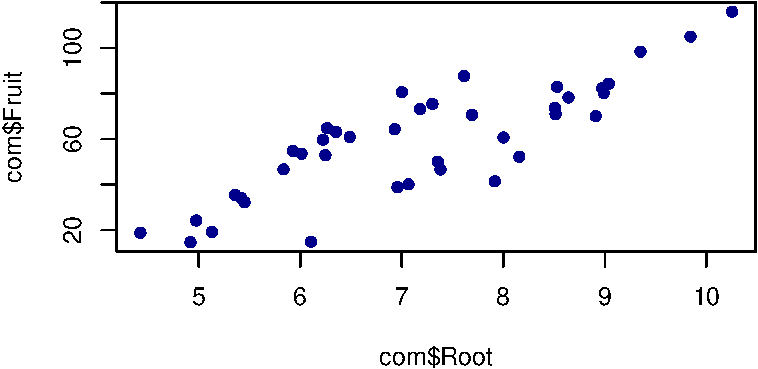
\includegraphics{statistics_files/figure-pdf/unnamed-chunk-21-1.pdf}

Bigger roots produced more seeds

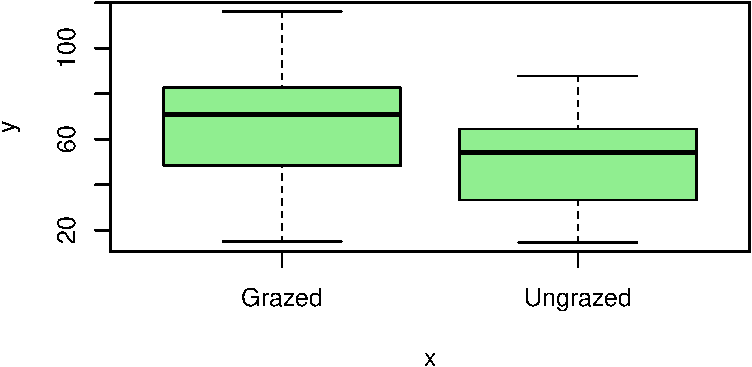
\includegraphics{statistics_files/figure-pdf/unnamed-chunk-22-1.pdf}

\begin{verbatim}
  Grazed Ungrazed 
 67.9405  50.8805 
\end{verbatim}

It seems that the grazed plants produced more fruits. Lets do the ANOVA

\begin{verbatim}
            Df Sum Sq Mean Sq F value Pr(>F)  
com$Grazing  1   2910  2910.4   5.309 0.0268 *
Residuals   38  20833   548.2                 
---
Signif. codes:  0 '***' 0.001 '**' 0.01 '*' 0.05 '.' 0.1 ' ' 1
\end{verbatim}

It is indeed significant from ANOVA.

Lets do the ANCOVA, we use the most complex model, two intercept and two
slopes for the grazed and ungrazed (use asterisk*). in ANCOVA, order of
the explanatory variables matter.

\textbf{ROOT} first

\begin{verbatim}
                     Df Sum Sq Mean Sq F value   Pr(>F)    
com$Root              1  16795   16795 359.968  < 2e-16 ***
com$Grazing           1   5264    5264 112.832 1.21e-12 ***
com$Root:com$Grazing  1      5       5   0.103     0.75    
Residuals            36   1680      47                     
---
Signif. codes:  0 '***' 0.001 '**' 0.01 '*' 0.05 '.' 0.1 ' ' 1
\end{verbatim}

\textbf{Grazing} first

\begin{verbatim}
                     Df Sum Sq Mean Sq F value   Pr(>F)    
com$Grazing           1   2910    2910  62.380 2.26e-09 ***
com$Root              1  19149   19149 410.420  < 2e-16 ***
com$Grazing:com$Root  1      5       5   0.103     0.75    
Residuals            36   1680      47                     
---
Signif. codes:  0 '***' 0.001 '**' 0.01 '*' 0.05 '.' 0.1 ' ' 1
\end{verbatim}

Both produces similar error sum of square (1680) and interaction sum of
squares (5). The regression sum of square where higher when root fitted
after grazing (19149) then before grazing (16795) due to non-orthogonal
data.

The SSRdiff, representing differences in slope between grazed and
ungrazed treatments appear insignificant, thus we can remove it. Then we
fit difference intercepts for grazed and ungrazed plants but fit the
same slope to both graphs (we use + sign in formula):

\begin{verbatim}
            Df Sum Sq Mean Sq F value  Pr(>F)    
com$Grazing  1   2910    2910   63.93 1.4e-09 ***
com$Root     1  19149   19149  420.62 < 2e-16 ***
Residuals   37   1684      46                    
---
Signif. codes:  0 '***' 0.001 '**' 0.01 '*' 0.05 '.' 0.1 ' ' 1
\end{verbatim}

Does the simpler model have significantly lower explanatory power? we
use anova:

\begin{verbatim}
Analysis of Variance Table

Model 1: com$Fruit ~ com$Grazing * com$Root
Model 2: com$Fruit ~ com$Grazing + com$Root
  Res.Df    RSS Df Sum of Sq      F Pr(>F)
1     36 1679.7                           
2     37 1684.5 -1   -4.8122 0.1031   0.75
\end{verbatim}

the simpler model does not produce lower explanatory power (p = 0,75),
thus we can adopt it.

if we see the linear model of model2

\begin{verbatim}

Call:
lm(formula = com$Fruit ~ com$Grazing + com$Root)

Residuals:
     Min       1Q   Median       3Q      Max 
-17.1920  -2.8224   0.3223   3.9144  17.3290 

Coefficients:
                    Estimate Std. Error t value Pr(>|t|)    
(Intercept)         -127.829      9.664  -13.23 1.35e-15 ***
com$GrazingUngrazed   36.103      3.357   10.75 6.11e-13 ***
com$Root              23.560      1.149   20.51  < 2e-16 ***
---
Signif. codes:  0 '***' 0.001 '**' 0.01 '*' 0.05 '.' 0.1 ' ' 1

Residual standard error: 6.747 on 37 degrees of freedom
Multiple R-squared:  0.9291,    Adjusted R-squared:  0.9252 
F-statistic: 242.3 on 2 and 37 DF,  p-value: < 2.2e-16
\end{verbatim}

The model has high explanatory variables, accounting for 93\% variation
(multiple r squared). The intercept (-127.8) is the intercept for the
graph of fruit production against plant rootstock size for the grazing
variable which the factor level whose come first (in this case grazed).

\begin{verbatim}
[1] "Grazed"   "Ungrazed"
\end{verbatim}

The
com\(GrazingUngrazed is the difference in intercept for the ungrazed plants (-127.8 + 36.1 = -91.726).
THe com\)Root is the slope, the gradient of fruit production against
initial rootstock size. It is same for both grazed or ungrazed, if it is
difference it will showed in the fourth row the difference between
slopes.

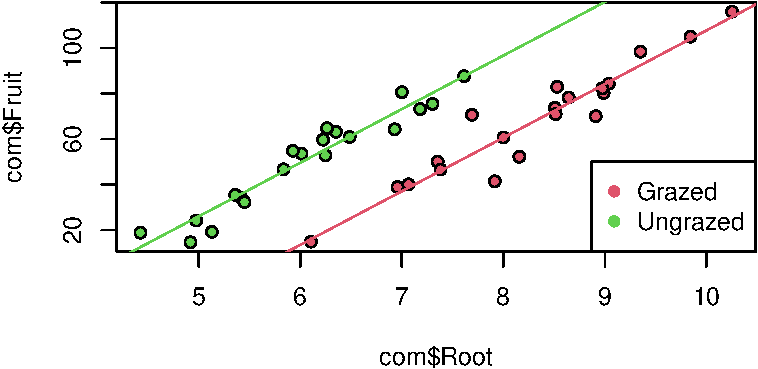
\includegraphics{statistics_files/figure-pdf/unnamed-chunk-30-1.pdf}

This showed that, the Grazed plants had relatively larger rootstock size
then ungrazed plants, thus explain why in the boxplot of fruit
\textasciitilde{} grazing showed that grazed plants produce more fruits
while it actually reduce fruit production.

\section*{Multiple Regression}\label{multiple-regression}
\addcontentsline{toc}{section}{Multiple Regression}

\markright{Multiple Regression}

\section*{Contrast}\label{contrast}
\addcontentsline{toc}{section}{Contrast}

\markright{Contrast}

\section*{Other Response Variables}\label{other-response-variables}
\addcontentsline{toc}{section}{Other Response Variables}

\markright{Other Response Variables}

\section*{Count Data}\label{count-data}
\addcontentsline{toc}{section}{Count Data}

\markright{Count Data}

\section*{Proportion Data}\label{proportion-data}
\addcontentsline{toc}{section}{Proportion Data}

\markright{Proportion Data}

\section*{Binary Response Variable}\label{binary-response-variable}
\addcontentsline{toc}{section}{Binary Response Variable}

\markright{Binary Response Variable}

\section*{Death and Failure}\label{death-and-failure}
\addcontentsline{toc}{section}{Death and Failure}

\markright{Death and Failure}

\chapter{Basic R and Base Plot}\label{basic-r-and-base-plot}

\chapter{Tidyverse \& ggplot2}\label{tidyverse-ggplot2}

\part{Mata Kuliah Dasar Umum}

Mata kuliah disampaikan kepada seluruh PPDS pada bulan pertama semester
satu.

Materi terdiri dari 5 bidang:

\begin{enumerate}
\def\labelenumi{\arabic{enumi}.}
\tightlist
\item
  Filsafat Ilmu
\item
  Biologi Molekuler2
\item
  Statistik Dasar
\item
  Metode Penelitian
\item
  Evidence-based Medicine
\end{enumerate}

\chapter{Biologi Molekular}\label{biologi-molekular}

\section{Cell Structure \& Organel}\label{cell-structure-organel}

Tujuan: memahami teknik teknik biologi molekuler untuk kepentingan
klinis.

Sel: bagian terkecil fungsional penyusun organisme

\textbf{Prokaryotic} - ukuran diameter 0.2 - 2.0 mikrometer - no nuclear
membrane - DNA sirkuler - etc

\textbf{Eukaryotic} - ukuran diameter 10 - 100 mikrometer - ada nuclear
membrane - DNA dalam kromosom - etc

\subsection{Organel Sel}\label{organel-sel}

\begin{enumerate}
\def\labelenumi{\arabic{enumi}.}
\tightlist
\item
  Inti Sel
\end{enumerate}

terdapat kromosom, mengandung DNA, protein histone dan non histone.

Central Dogma: DNA ditrankripsi menjadi mRNA DNA direplikasi menjadi
kopi DNA lain

mRNA akan di translasi menjadi Protein,

Jenis RNA: mRNA, tRNA, rRNA, miRNA, siRNA

\begin{enumerate}
\def\labelenumi{\arabic{enumi}.}
\setcounter{enumi}{1}
\tightlist
\item
  Membran sel
\end{enumerate}

Terdiri dari Fosfolipid bilayer, protein integral \& perifer,

\begin{enumerate}
\def\labelenumi{\arabic{enumi}.}
\setcounter{enumi}{2}
\item
  Sitoplasma
\item
  Ribosom subunit kecil dan besar bersatu menjadi kompleks. Ribosom bisa
  menmpel pada RE kasar.
\item
  retikulum endoplasma
\item
  mitokondria
\item
  Badan Golgi
\item
  Lisosom
\item
  Peroksisom
\end{enumerate}

\section{Genome Organization}\label{genome-organization}

Genome =\textgreater{} chromosome =\textgreater{} Chromatin
=\textgreater{} Gene

\textbf{Gen vs DNA}

\begin{itemize}
\tightlist
\item
  Gen = unit fungsional dan struktural hereditas
\item
  DNA = Struktur template RNA
\end{itemize}

Ukuran panjang DNA nukleus =\textgreater{} 3200 million base pair ukuran
panjang DNA mitokondria =\textgreater{} 16.6 kilo base pair

\begin{figure}

\centering{

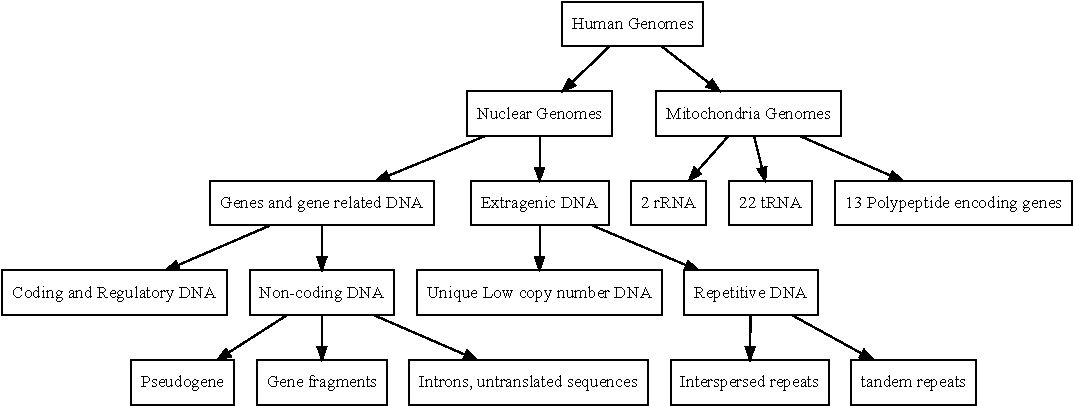
\includegraphics{biomol_files/figure-pdf/fig-genomes-1.pdf}

}

\caption{\label{fig-genomes}Human Genomes}

\end{figure}%

pol 1 mRNA pol 2 lain lain pol 3 rRna

\subsection{Protein coding genes}\label{protein-coding-genes}

\begin{itemize}
\tightlist
\item
  Genes memiliki exon dan intron, ukuran bervariasi
\item
  ada genes yang tidak memilili intron =\textgreater{} gene coding
  histone
\item
  gene yang berukuran besar, pengkode dystropin, 99\% menganding intron
\item
  Gen yang sering di transkripsi biasanya memiliki intron yang pendek
\end{itemize}

\textbf{RNA Coding Sequence} DNA =\textgreater\textgreater{} Enhancer --
Promoter ---------------------------------------------------------------
terminator

transkripsi

pre-RNA =\textgreater\textgreater{} 5'cap -- leader --
exon-intron-exon-intron-exon-intron-exon-intron---trailer--- poly A tail
3' cap dan poly A tail ditambah post transkripsi

mature mRNA 5'cap -- leader -- exon---trailer--- poly A tail 3'

translasi di sitoplasma

mRNA =\textgreater{} monosistronik = 1 untai RNA menyandi 1 gen
=\textgreater{} manusia, polisistronik di prokaryotic

\subsection{Codon}\label{codon}

1 kodon terdiri dari 3 basa. terdapat 64 kodon, termasuk 3 stop kodon
Lihat tabel kodon

\section{DNA \& RNA Structure}\label{dna-rna-structure}

Central dogma\ldots\ldots\ldots{}

\section{Signal Transduction}\label{signal-transduction}

Komponen membran Sel:

\begin{itemize}
\tightlist
\item
  Phospolipid bilayer bersifat amphiphatic yaitu ada sisi hidrofobik dan
  sisi hidrofilik. Komponen terdiri dari

  \begin{itemize}
  \tightlist
  \item
    Phospate Head
  \item
    Glycerol Backbone
  \item
    Fatty Acid Tails
  \end{itemize}
\item
  Protein:

  \begin{itemize}
  \tightlist
  \item
    Integral protein, melewati 2 lapir membran
  \item
    Peripheral protein, menempel hanya pada 1 lapis membran
  \end{itemize}
\end{itemize}

Sifat fosfolipid semipermeable, yakni permeable terhadap zat selektif. -
Small non polar, mudah melewati membran (Co2, O2) - Small polar, bisa
melewati membran tapi lambat (ethanol) - Large Non-polar - Large Polar -
Charged

Komponen sel signalling

\begin{enumerate}
\def\labelenumi{\arabic{enumi}.}
\item
  Signal
\item
  Reseptor Sensing the signal. Terjadi perubahan struktur reseptor saat
  berinteraksi dgn signal

  \begin{itemize}
  \tightlist
  \item
    2 tipe reseptor

    \begin{itemize}
    \item
      Intraseluler/cytosolic receptor eg. steorid hormone
    \item
      ekstraseluler/transmembrance/cell surface membrane receptor eg.
      polypetide hormone (insulin, glukagon).

      Tipe transmemberane reseptor:

      \begin{itemize}
      \tightlist
      \item
        Ion channel linked receptor
      \item
        G Protein Linked Receptor, aktivasi protein meningkatkan
        konsentrasi second messenger, terjadi proses amplifikasi signal.
      \item
        Enzyme Linked Receptor, signal mengaktivasi aktivitas enzim yang
        juga menjadi reseptor. contoh : tyrosine kinase, phospolipase C
        memotong PIP2 menjadi IP3 dan DAG
      \end{itemize}
    \end{itemize}
  \end{itemize}
\end{enumerate}

to continued\ldots..

\section{Cell Cycle}\label{cell-cycle}

Siklus sel terdiri dari 2 tahap besar yaitu replikasi DNA dan segregasi
sel. Siklus sell terdiri dari 4 fase: G1, S, G2 dan M. Proses siklus sel
bukan hanya pembelahan, tetapi juga terkait dengan pertumbuhan sel dan
proses lainnya.

Proses melibatkan poerubahan chromatin dari closed conformation
(heterochromatin) yang sulit mengalami transkripsi (represed) menjadi
Euchromatin (open chromatin) atau mudah transkripsi (activation)

Terdapat beberapa checkpoint siklus sel. checkpoints ukuran sel (protein
dll, massa ribosomal), DNA damage. DNA damage bisa akibat:

\begin{itemize}
\tightlist
\item
  faktor intrinsik
\item
  faktor extrinsik
\item
  Kontrol dari protein: p53 chk1
\end{itemize}

Faktor lain berpengaruh terhadap siklus sel - mutasi faktor checkpoint -
epigenetic - aktivitas histon - smallDNA atau smallRNA, panjang 10-25
nucleotida, berfungsi mengenali transkrip untuk memotong mRNA yang
sesuai.

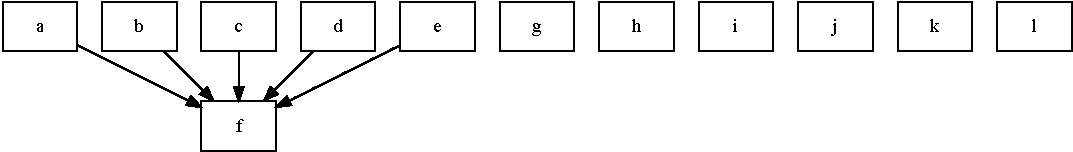
\includegraphics{biomol_files/figure-pdf/unnamed-chunk-2-1.pdf}

\subsection{G1}\label{g1}

Fase Gap 1, menentukan apakah pasien akan masuk ke tahap pembelahan.
Jika ada kondisi yang tidak optimal, maka sel tidak akan masuk ke
pembelahan. Durasi paling panjang ada pada G1 (12-15 hrs)

Ada peran dari fosforilasi protein retinoblastoma (RB) oleh protein CDKs
(cyclin dependent kinases.

Cyclin berikatan dengan CDKS, mengaktifkan CDK, CDK lalu melakukan
fosforilasi enzim enzim terkait. CDK adalah kelompok serine/theronine
protein kinases.

CDK 4/6 dan cyclin D dari unphosphorylated pRB menjadi hypofosforilasi
pRb, oleh CDK4/6-cyclinD CDK 2 - cyclin E (post Repclication point)

Perain penting protein p53 dan Mdm2 pada G1. P53 penting juga pada fase
G2 jika ada yang terlewat pada fase G1. p53 berfungsi posttranslational
medification, termasuk fosforilasi.

\subsection{S}\label{s}

durasi 6-8 jam

CDK 2 dan cyclin A dari hypo menjadi hyperforilasi pRb, oleh
CDK2-cyclinA

\subsection{G2}\label{g2}

Durasi 3-5 jam

CDC2 - cyclin A hyperforilasi pRb

\subsection{M}\label{m}

Durasi 1 jam CDC2 - cyclin B hyperforilasi pRb

post M, defosforilasi pRB

\section{Mutastion \& Free Radical \&
Antioksidan}\label{mutastion-free-radical-antioksidan}

Mutasi basa: substitusi, delesi, insensi.

\subsection{SUbstitusi biasanya terjadi 1 basa saja, sehingga sering
juga disebut point
mutation.}\label{substitusi-biasanya-terjadi-1-basa-saja-sehingga-sering-juga-disebut-point-mutation.}

Substitusi bisa transversi menjadi transisi. Transisi: purin
\textgreater{} purin Transversi: purin \textgreater{} pirimidin atau
sebaliknya.

Hasil preotein: Silent mutation: asam amino sama Missense mutation:
berubah kode asam amino Nonsense mutation: berubah menjadi stop kodon
stop codon mutation: merubah stop kodon menjadi kodon asam amino.

\subsection{Delesi dan Insersi}\label{delesi-dan-insersi}

Delesi dan insersi mengubah reading frame, sehingga disebut dengan
frameshift mutation.

\subsection{}\label{section-1}

\subsection{Molecular effect of
Mutation}\label{molecular-effect-of-mutation}

Within coding region - Silent (biasanya mutatasi pada basa ketiga di
kodon, sering tidak mengganti asam amino) - Missense - Non-sense
(premature stop codon) - Frameshift

Within non-coding region - SPlicing mutation - Regulatory Sequence
mutation

\subsection{Clinical Effect of
Mutation}\label{clinical-effect-of-mutation}

\begin{itemize}
\tightlist
\item
  Acceptable
\item
  Partially acceptable
\item
  Unacceptable (fatal/letal)
\end{itemize}

bisa menumbulkan kanker, inborn error metabolism.

Kanker muncul: - altered protein

\subsection{DNA Repair}\label{dna-repair}

\subsubsection{SPontaneous Mutation}\label{spontaneous-mutation}

\begin{itemize}
\tightlist
\item
  Mismatch Repair DNA kita secara natural ada metilasi, jika belum
  termetilasi setelah replikasi maka akan di excisi oleh endonuclease.
\end{itemize}

\subsubsection{Metagen}\label{metagen}

\begin{itemize}
\tightlist
\item
  Photoreactivation Timin Dimer, dipotong pada dimernya lalu dilakukan
  excision repair.
\end{itemize}

Tipe Repair - Base excision repor - Nucleotide excision repair.

\subsection{Free Radical}\label{free-radical}

Molekul yang memiliki elektron yang tidak berpasangan di orbit
terluarnya. Radikal bebas tidak stabil, sehingga mencuri elektron dari
molekul lain, dan mencipkan radikal bebas lain.

Oksidant: elektron acceptor, Fe3+ + e =\textgreater{} Fe2+

Sifat: 1. Highly reactive, 2. Unstable 3. Very short half-life 4.
Generate new radicals by chain reaction 5. Cause damage to biomolecules,
cells

\subsubsection{Reactive Oxygen Species
(ROS)}\label{reactive-oxygen-species-ros}

\begin{itemize}
\tightlist
\item
  H2O2
\end{itemize}

ada juga Reactive nitrogen species

Sulit diperiksa secara langsung. Pemeriksaan secara tidak langsung
dengan pemeriksaan produk dari hasil paparan radikal bebas.

Sumber radikal bebas: - Mitokondria pada proses pembentukan ATP,

\subsubsection{Sumber Radikal Bebas}\label{sumber-radikal-bebas}

\begin{itemize}
\tightlist
\item
  Endogen
\item
  EKsogen
\end{itemize}

\section{DNA Replication}\label{dna-replication}

Replikasi DNA terjadi pada fase S pada siklus sel bertujuan membuat copy
DNA untuk diwarikan ke sel keturunanya.

\section{Mutation \& DNA Repair}\label{mutation-dna-repair}

\section{Gene Expression}\label{gene-expression}

Jumlah gene sel manusia ada sekitar 20 rb - 30 rb. Setiap sel somatik
sama jumlahnya, yang berbeda adalah aktivasinya pada masing-masing tipe
sel.

Proses transkripsi: ada inisiasi, elongasi dan terminasi. Proses
translasi: iniasi, elongasi, terminasi

\subsection{Transkripsi}\label{transkripsi}

\subsubsection{Inisiasi}\label{inisiasi}

RNA Pol 1, RNA pol 2, RNA pol 3.

Promoter mengenali sekuens DNA spesifik yang disebut responsive element
dalam proses inisiasi transkripsi. Ada komples TATAA Box. Kompleks
promotor menarik aparatus faktor faktor yang membentu proses
transkripsi. Selain promotor adalah enhancer. Enhancer terletak lebih
jauh dari gene terkait, baik upstream atau downstream yang membentuk
sebuah DNA loop berikatan dengan kompleks inisiasi.

\subsubsection{Elongasi}\label{elongasi}

\subsubsection{Terminasi}\label{terminasi}

Terminasi terjadi karena pemotongan strand RNA pada sekuens tertentu.
RNA kemudian ditambah poly A tail untuk meningkatkan stabilitas. Makin
panjang Poly A tail, makin stabil.

\subsubsection{Post transcriptional Step in Gene
Expression.}\label{post-transcriptional-step-in-gene-expression.}

\begin{enumerate}
\def\labelenumi{\arabic{enumi}.}
\tightlist
\item
  mature RNA megalami splicing
\item
  Penambahan 5' end cap, menjadi 7 mentilguanosin cap
\item
  Penambahan 3' poli adenin tail
\end{enumerate}

Terjadi regulasi paska transkripsi melibatkan small/micro RNA.

\subsection{Translasi}\label{translasi}

\subsection{Regulasi Transkripsi}\label{regulasi-transkripsi}

Regulasi mRNA tergantung 1. kestabilan mRNA 2. pasangan mirna (RNAi) 3.
keadaan sel 4. Metilasi DNA (pada sitosin)

Transcription control of genes transcriptional regulation occurs at two
interconnected levels - Histon complex - \textbf{histon COde} -

\section{Control of Gene Expression}\label{control-of-gene-expression}

\section{Genetic Variation}\label{genetic-variation}

Microevolution is a change in allele frequencies in a population over
generations. Three mechanism:

\begin{itemize}
\tightlist
\item
  Natural Selection
\item
  Genetic Drift
\item
  Gene flow
\end{itemize}

only natural selection causes adaptive evolution. Hardy - Winberg
Equilibrium: genetic variation will remain constant from one generation
to the next in the absence of disturbing factors.

\section{Genotyping}\label{genotyping}

Process determining the genetic constitution of an individual and
comparing to the other individual or reference sequence. Perbedaan
interspesies \textless1\%.

Genotyping pada manusia untuk mengetahui susceptibilitas atas penyakit
dan response terhadap pengobatan.

\subsection{Polimorfisme vs Mutasi}\label{polimorfisme-vs-mutasi}

Perubahan basa DNA, mutasi perubahan sekuens dari normal. Polimorfisme
adalah perubahan basa yang merupakan variasi normal. Cut-off point
antara mutasi dan polimorfisme adalah 1\%, artinya variasi alele
setidaknya memiliki frekuensi minimal 1\% di populasi.

Polimorfisme bisa berupa silent point mutation.

\subsubsection{SNP}\label{snp}

Variation when a single nucleotide in genome is altered. SNP do not
always affect the way protein functions.

\begin{itemize}
\tightlist
\item
  Linked SNP/Indicative SNP : do not reside within genes, do not affect
  protein function, but correspond to certain characteristics
\item
  Causative SNP: affect the way protein functions, whether:

  \begin{itemize}
  \tightlist
  \item
    Coding SNP: located in coding region, changes the amino acid
    sequence
  \item
    Non-coding SNP: within gene regulatory sequences: change timing and
    expression of gene.
  \end{itemize}
\end{itemize}

\section{Stem Cell}\label{stem-cell}

Sel yang belum terspesialisasi.

\begin{itemize}
\tightlist
\item
  Ebroyonic Stem Cells ( inner cells mass)
\end{itemize}

\section{Molecular Biology Technique}\label{molecular-biology-technique}

DNA universal

\section{Aplication of Molecular Biology in
Medicine}\label{aplication-of-molecular-biology-in-medicine}

\chapter{Metodologi Penelitian}\label{metodologi-penelitian}

\section{Overview of Clinical
Research}\label{overview-of-clinical-research}

clinical research is medical research taht involves people, to learn
more about disease and improve health care for people in the future.

include: epidemiology, behavioral, health services, clinical trials.

clinical research, not just clinical trial, it is any research design
that studies humans or any materials taken from humans. it may even
include animal studies that the results apply to humans.

type of clinical research:

\begin{itemize}
\tightlist
\item
  observational studies =\textgreater{} studies that aim to identify and
  analylyze patterin medical data.
\item
  clinical trials/interventional studies
\end{itemize}

Research Question: FINER - Feasible - interesting - novel - ethical -
relevant

\section{Association \& Causation}\label{association-causation}

Sebuah hubungan belum tentu menunjukan sebab-akibat. Banyak peneliti
menghindari dgmatic statement: ``cause'' or ``produces''

Causation: occurs when a change in one variable produces a change in
another variable

\begin{itemize}
\tightlist
\item
  Contributory Cause, no single specific cause of a disease. Most of
  disease cause by multifactorial etiologies. A risk factor may a
  contributory cause.
\end{itemize}

Three criteria: 1. Association may be reflected by effect size 2. Prior
Association, does the cause (independent var) precede the effects
(dependent var) (case control or cohort), 3. Altering the cause alters
the effects

Some other features of contributory causation:

\begin{enumerate}
\def\labelenumi{\arabic{enumi}.}
\item
  Consistency: the results of study (effect size) should be consistent
  regardless the design, the population used.
\item
  Dose response relathionsip
\item
  Biologic Plausibility: should make biologic sense.
\item
  Experimental confirmation: phenomenon found in lcinical studies have
  to be consistent with studies in animal models.
\end{enumerate}

\begin{itemize}
\tightlist
\item
  Necessary cause, dibuktikan sebagai satu satunya penyebab. Sebagai
  contoh: fullfiled by Koch's Postulates: the organism is always found
  with the disease.
\end{itemize}

Association: can be observed between many variable, but causaton only be
determined from data collected from a controlled experiment.

\begin{itemize}
\item
  Spurious association, association no actually present in population 3
  mekanisme spurious causation

  \begin{itemize}
  \item
    Chance, due to random error and sampling variation (Individual
    chance to be a sample not equal), karakteristik sampel terlalu
    heterogen. Minimize random error: adequate sample size and low type
    1 and type 2 error. Effect of random error can be judged from the
    width of the 95\% confidence interval and the consistency of the
    results with previous evidence.
  \item
    Design, conduct of the study, and analyze of the results,

    \begin{itemize}
    \tightlist
    \item
      selection bias, pemilihan sampel yg tidak sesuai =\textgreater{}
      randomized and blind intervention
    \item
      performance bias, pemberian intervensi tidak setara antar sampel
      =\textgreater{} randomized and blind intervention
    \item
      Detection bias, deteksi efek atau cause tidak sama =\textgreater{}
      randomized and blind intervention
    \item
      Transfer bias, loss to follow up
    \end{itemize}
  \item
    Confounding, occurs when factors which related to both independent
    and dependent variables. Contoh Kopi menyebabkan AMI, tetapi ada
    faktor merokok dimana orang ngopi juga suka merokok. Ternyata
    merokok yang berhubungan dgn AMI, tetapi merokok tidak berhubungan
    dengan AMI. Kontrol dengan by design atau by analysis.
  \end{itemize}
\item
  Real Association, true biological phenomena. However not due to a
  cause effect relationship
\end{itemize}

\textbf{Critical Appraisal about Harm/Etiology/Causation.} follow
checklist.

PR: 1 jenis penelitian causation atau association yang menjadi ide
kalian nanti penelitian.

\section{Research Measurement}\label{research-measurement}

\section{Variables and Relathionship Between
Variables}\label{variables-and-relathionship-between-variables}

Variable: independent, dependent, confounding variables

other variable: mediator, moderator, external, random

relathioships among variables

\begin{itemize}
\tightlist
\item
  chances
\item
  bias
\item
  confounding
\item
  causal
\end{itemize}

\section{Hypothesis and Hypothesis Testing \& Effect Size, Confident
Interval, and P
Value}\label{hypothesis-and-hypothesis-testing-effect-size-confident-interval-and-p-value}

Hypothesis:

a statement about relathionsip between two or more variables that
suggest an answer to the research question, is declarative statement
that predicts an expected outcome.

Research hypothesis: kalimat deklaratif yang mencoba memberikan jawaban
sementara atas pertanyaan penelitian.

Statistical hypotesis: biasanya tidak ditulis di proposal.

Research hypothesis nanti akan di uji apakah hypotesis didukukng oleh
data data.

Jika hypotesis yang kita uji tidak sesuai dengan data, maka bukan
berarti ilmu itu salah

\section{Sample Size and Power}\label{sample-size-and-power}

Sample size pentingnya untuk bisa mewakili populasi dan dapat inferensi
ke populasi itu kembali, serta:

\begin{itemize}
\tightlist
\item
  untuk mendeteksi treatment effects jika memang ada di populasi
  (mendapatkan hasil statistik signifikan dan secara klinis penting)
\item
  Presisi estimasi
\item
  avoid wasting resources
\item
  avoid misleading conclusion
\end{itemize}

\textbf{Two many subject proves everything, too few subject proves
nothing}

Kapan ketika perhitungan sample size tidak diperlukan? - Penelitian
kualitatif - Pilot studi, biasanya 10 -20 subjek untuk menentukan sample
size studi yang lebih besar.

Sampel size sesuai dengan design, analysis plan dan outcome. Sample size
harus sesuai untuk memenuhi statistical significance dan clinically
important, tanpa membuang sumber daya terlalu banyak.

Sampel size berhubungan power. Power = makin kuat penelitian mampu
mendeteksi sebuah efek di populasi, maka semakin banyak sample size
dibutuhkan.

Definition of Power: the probability of concluding the new treatment is
effective if it truly is effective. Biasanya 80\% type I error = the
probability of concluding that the new treatment is effective if it
truly is not effective. (positive palsu, alpha) type II error = the
probability of concluding the new treatment not effective if it is truly
effective (negative palsu, 1 - power atau beta)

Elemen menentukan sample size: \(\Delta\) = \textbf{effect size} or
difference under null hypotesis (perbedaan klinis yang dianggap penting)
diambil dari studi sebelumnya dan tinjauan pustaka. Jika effect size
besar, maka sampel di butuhkan lebih kecil, begitu kebalikannya
\(\alpha\) = type I error, 0,05 \(\beta\) = type 2 error, 0,2 \(\sigma\)
= standard deviation, makin heterogen populasi maka sample size makin
besar. r = ratio of number of patients in the two groups, usually r = 1

Hubungan sampel size dengan hasil presisi, dimana hasil confidence
interval akan lebih sempit (lebih presisi) jika sample size besar. Jika
hipotesis 2 arah, sample lebih besar, biasanya lebih disarankan
hipotesis 2 arah. Pertimbangan tambahan sampel jika kemungkinan loss to
follow up terutama pada kohort prospektif dan clinical trial. Jika cross
sectional, tidak perlu. Jika tidak ada studi sebelumnya sebagai patokan
sampel, maka tetap harus memperhitungkan sampel dengan cara pilot study.

Jika tidak bisa memenuhi jumlah sampel sesuai perhitungan sebelum
penelitian (apriori), kita bisa mennetukan apakah hasil studi kita
underpower dengan memperhitungkan hasil tes post-hoc.

Stategi meminimalkan sample size - pakai varibael kontinyu - paired
measurement.

rule of thumb: 10 - 50 per variabel, atau 30 sampel. Pakai rule of thumb
jika tidak ada data yang bisa mendukung perhitungan jumlah sampel.

Effect size tidak boleh mengutip dari penelitian lain secara
\emph{eksplisit} di proposal.

\section{Research Design}\label{research-design}

Jenis penelitian digunakan untuk membuktikan tujuan penelitian.

Sebainya tidak perlu dilakukan analisis untuk mendapatkan nilai P untuk
membandingkan karakteristik sampel antar 2 kelompok sebagai usaha untuk
menunjukan 2 kelompok tersebut komparabel, jika kita tidak
menghipotesiskan seperti itu.

Desain:

\subsection{Cross sectional}\label{cross-sectional}

Pengukuran variabel bebeas dan tergantung terjadi bersamaan. Baik untuk
penyakit yang durasi sakitnya lama, dan kejadian cukup banyak.

\subsection{Kasus-Kontrol}\label{kasus-kontrol}

Identifikasi sampel dengan variabel tergantung dulu, kemudian dicari
kontrolnya, lalu dilihat secara retrospektif mencari variabel bebasnya.
Lalu dihitung rasio odds. Odds: Perbandingan terjadinya efek
dibandingkan tidak terjadinya efek pada suatu kelompok Rasio Odds:
perbandingan odds antar 2 kelompok.

Matching case control:

Variabel bebas bisa banyak

\subsection{kohort}\label{kohort}

Mengidentifikasi variabel bebas, lalu diobersevari untuk melihat
variabel tergantung. Baik untuk kasus yang jarang, dan perjalananya
penyakit jarang.

Variabel tergantung bisa banyak

\subsection{Nested Case-Cohort Study atau Nested Control
Study}\label{nested-case-cohort-study-atau-nested-control-study}

Umumnya penelitian yang sampelnya bisa disimpan di Lab dan
pemeriksaannya mahal. Controlnya: di matching =\textgreater{} case
cohort study Controlnya: di Random =\textgreater{} case control study

\subsection{Uji Diagnostik}\label{uji-diagnostik}

Selalu tabel 2 x 2.

\section{Cross Sectional \& Case-Control
Study}\label{cross-sectional-case-control-study}

\subsection{Cross-sectional Study}\label{cross-sectional-study}

Cross sectional study assessing prevalence (old and new patient).

\begin{enumerate}
\def\labelenumi{\arabic{enumi}.}
\tightlist
\item
  Formulate appropriate research question and hypothesis
\item
  Identify indepent and dependent variables
\item
  Determine research subjects
\item
  Carry out measurements
\item
  Do analysis
\end{enumerate}

Tabel 2x2 harus risk factor di kiri, effect di atas.

\begin{center}\rule{0.5\linewidth}{0.5pt}\end{center}

\subsection{Case-Control Study}\label{case-control-study}

\section{Cohort Study}\label{cohort-study}

\section{Experiments}\label{experiments}

\section{Diagnostic Test}\label{diagnostic-test}

\section{Data Management and
Analysis}\label{data-management-and-analysis}

\section{Research Proposal}\label{research-proposal}

\section{Ethical Issue}\label{ethical-issue}

\section{Novelty Aspect}\label{novelty-aspect}

\chapter{Filsafat Ilmu}\label{filsafat-ilmu}

\section{Pengantar Filsafat Ilmu}\label{pengantar-filsafat-ilmu}

Filsafat ilmu: untuk mencari tujuan hidup.

\textbf{Ontology} : study of existence, becoming and reality, mengetahui
segala sesuatu yang ada sebagaimana adanya. \textbf{Mencari tahu tentang
hal terkait}. \textbf{Epistemology} : Study of knowledge, bagaimana kita
bisa mendapatkan pengetahuan yang hakiki itu atau sesuatu yang ada
sebagai mana adanya. \textbf{Mengetahui semua hal untuk mencapai
sesuatu/how to achieve it.}

Deduktif: Mencari ke arah spesifik

Induktif: Mencari teori (ke arah umum)

\textbf{Aksiology} : Study of Value, ilmu pengetahuan yang didapat itu
bisa diterapkan untuk kemahaslatan umat atau justru sebaliknya.
\textbf{bagaimana cara menggunakan ilmunya}

pengetahuan +\textgreater{} 5 panca indra, pengetahuan bisa menjadi ilmu
jika melalui ilmiah dan dapat diturunkan/semua bisa mempelajari dengan
hasil yang sama.

Filsafat ilmu sebagai kumpulan teori digunakan memahami dan mereaksi
dunia pemikiran.

\section{Ilmu Sebagai Produk
Berpikir}\label{ilmu-sebagai-produk-berpikir}

\section{Ilmu dan Teknologi
Kedokteran}\label{ilmu-dan-teknologi-kedokteran}

\section{Ontologi, Epistemologi, dan Aksiologi
Kedokteran}\label{ontologi-epistemologi-dan-aksiologi-kedokteran}

\section{Intelektualitas dan Aktivitas
Intelektual}\label{intelektualitas-dan-aktivitas-intelektual}

\section{Pengetahuan dan Ilmu
Pengetahuan}\label{pengetahuan-dan-ilmu-pengetahuan}

\section{Teori Kebenaran Ilmiah}\label{teori-kebenaran-ilmiah}

\section{Perkembangan Ilmu
Kedokteran}\label{perkembangan-ilmu-kedokteran}

\section{Aksiologi, Sikap Ilmiah dan Etika
Ilmiah}\label{aksiologi-sikap-ilmiah-dan-etika-ilmiah}

\section{Complementary \& Alternative
Medicine}\label{complementary-alternative-medicine}

\section{Komunikasi Ilmiah}\label{komunikasi-ilmiah}

\section{Bioetika Penelitian}\label{bioetika-penelitian}

\section{Publikasi dan Hak Paten}\label{publikasi-dan-hak-paten}

\section{Filsafat Ketuhatan dan
Kemanusiaan}\label{filsafat-ketuhatan-dan-kemanusiaan}

\section{Metode Penalaran Ilmiah}\label{metode-penalaran-ilmiah}

\chapter{Statistik Kedokteran Dasar}\label{statistik-kedokteran-dasar}

\section{Dasar-dasar Penulisan Ilmiah Kedokteran dan
Plagiarisme}\label{dasar-dasar-penulisan-ilmiah-kedokteran-dan-plagiarisme}

Metode sains: bisa diulang dengan hasil yang sama. observasi,
measurement, verification and evaluation (self correction)

\subsection{Methods of acquiring
knowledge}\label{methods-of-acquiring-knowledge}

\begin{itemize}
\tightlist
\item
  Method of Tenacity
\item
  Method of Authority
\item
  Method of Intuition
\item
  Method of Science
\end{itemize}

\subsection{Benefits of Conducting
Research}\label{benefits-of-conducting-research}

\begin{itemize}
\tightlist
\item
  Expanding frontiers of knowledge
\item
  New inventions and discoveries
\item
  Solving problems affecting the society
\item
  Increasing efficiency and reducing costs
\item
  Research strives to make life easier
\item
  Luxury and comfort
\item
  Infotainment
\item
  Economic growth
\end{itemize}

\subsection{Qualities of a researcher}\label{qualities-of-a-researcher}

\begin{itemize}
\tightlist
\item
  Scientific attitude
\item
  Research aptitude
\item
  Persistence
\item
  Self Motivation
\item
  Courage to ask questions
\item
  Skepticism and receptivity
\item
  Objectivity
\item
  Industriousness
\item
  Honesty and truthfulness
\item
  Open-mindedness
\item
  Above-average intelligence
\item
  Knowledge
\item
  Imagination
\item
  Self-confidence
\item
  Search for perfection
\item
  Team spirit
\end{itemize}

\subsection{Bioethical}\label{bioethical}

\begin{itemize}
\tightlist
\item
  Autonomy - consent to treatment
\item
  Beneficence
\item
  Justice
\item
  Utility - balancing benefit
\item
  Inform Consent
\item
  Confidentiality
\end{itemize}

\subsection{Induction and Deduction in
Research}\label{induction-and-deduction-in-research}

\begin{itemize}
\item
  Deductive reasoning is the process of reasoning from a general
  assumption to a specific application. Contoh: General proposition: all
  crows are black Specific proposition: this bird is a crow, therefore
  it is black
\item
  Indcution normally involves generalization from the behavior of a few
  samples to that of a population contoh: all jasmine flowers are
  scented, if a situation or condition is true in all observed cases,
  then the situation or condition must be true in all cases.
\item
  Hypothetico-deductive method or inductive-deductive method.
\end{itemize}

\subsection{Scientific Method}\label{scientific-method}

It should be unprejudice

\begin{itemize}
\tightlist
\item
  Make observations or gather information
\item
  Develop hypothesis
\item
  Predicts results
\item
  Design an experiment to falsify the hypothesis
\item
  Conduct the experiment and collect data
\item
  Evaluation and conclusion
\item
  Acceptance, modification or rejection of the hypothesis
\end{itemize}

\subsection{First Draft}\label{first-draft}

\begin{itemize}
\tightlist
\item
  Why did you start the experiment? (introduction)
\item
  What did you do? How was it done (The materials and methods)
\item
  What did you find? What was learned? (the results)
\item
  What do the results mean? How do they relate to what is already known?
  (the discussion)
\end{itemize}

\subsection{Structure of a Research
Paper}\label{structure-of-a-research-paper}

\begin{itemize}
\tightlist
\item
  Title
\item
  Running Title
\item
  Author
\item
  Institution
\item
  Abstract
\item
  Keywords
\item
  Introduction
\item
  Materials and Methods
\item
  Results
\item
  Discussion
\item
  Conclusion
\item
  Acknowledgements
\item
  References
\item
  Tables and Figures
\end{itemize}

\subsection{Seven Categories of
plagiarism}\label{seven-categories-of-plagiarism}

\begin{itemize}
\tightlist
\item
  direct plagiarism
\item
  mosaic plagiarism
\item
  paraphrase plagiarism
\item
  insufficient acknowledgement
\item
  complete plagiarism
\item
  self plagiarism
\item
  accidental plagiarism
\end{itemize}

\subsection{Characteristics of Good
Research}\label{characteristics-of-good-research}

\begin{itemize}
\tightlist
\item
  Research is based on the work of others
\item
  Research is a blend of logic and imagination
\item
  Research tries to identify and avoid bias
\item
  Repeatability
\item
  Research must be generalizable to other settings
\item
  Research is systematic
\item
  Research generates new questions
\item
  Research is an apolitical activity
\end{itemize}

\section{Kiat-kiat Publikasi Majalah Terakreditasi dengan
OJS}\label{kiat-kiat-publikasi-majalah-terakreditasi-dengan-ojs}

\subsection{Kendala Publikasi di
Indonesia:}\label{kendala-publikasi-di-indonesia}

\begin{itemize}
\tightlist
\item
  Indonesia lack of language access. Why we dont make one in Bahasa
  Indonesia?
\item
  Lack of Cultural backgroud dalam menulis.
\end{itemize}

\subsection{Kenapa publikasi penting?}\label{kenapa-publikasi-penting}

\begin{itemize}
\tightlist
\item
  Rekognisi atas hasil penelitian anda baik pengakuan regional, nasional
  dan internasional
\item
  H Index
\item
  Jaminan kolaborasi di tingkat regional, nasional, dan internasional
\end{itemize}

\subsection{Jurnal}\label{jurnal}

Jurnal biasanya di rangking berdasarkan dimana jurnal tersebut di
indeksasi (misal scopus, medline, ISI, Sinta, dll)

\subsubsection{Kriteria Jurnal
International}\label{kriteria-jurnal-international}

\begin{enumerate}
\def\labelenumi{\alph{enumi}.}
\tightlist
\item
  Tulisan memenuhi kaidah ilmiah dan etika keilmuan
\item
  Memiliki ISSN
\item
  Ditulis dengan bahasa resmi PBB (inggris, france, arab, rusia, and
  china)
\item
  Memiliki terbitas versi online
\item
  Dikelola secara profesional
\item
  Editorial board pakar di bidangnya, dan berasal dari berbagai negara
\item
  artikel ilmiah diterbitkan dalam satu isu berasal dari penulis
  berbagai negara
\item
  memuat karya ilmiah dari penulis yang berasal dari berbagai negara
  dalam setiap penerbitannya
\item
  Terindeks database international berputasi.
\end{enumerate}

Publikasi:

\begin{itemize}
\tightlist
\item
  Submit ke jurnal dgn OJS
\item
  Jika ditolak, edit ulang dan perbaiki.
\end{itemize}

Perlu diketahui: - Penulisan naskah/manuskrip ilmiah merupakan suatu
tangtangan, seni dan kemampuan mengelaborasi hasil penelitian. - Ikuti
kaidah IMRAD. Introduction biasanya sudah menggambarkan M,R,D nya.

Author vs Behavior

\begin{itemize}
\tightlist
\item
  Author

  \begin{itemize}
  \tightlist
  \item
    Want to publish more, write in detail
  \item
    peer review essential
  \item
    other journal functions crucial
  \item
    wider dissemination
  \end{itemize}
\item
  Reader

  \begin{itemize}
  \tightlist
  \item
    want to read less. (judul yg baik)
  \item
    Want integrated system
  \item
    Browsing is crucial
  \item
    Quality information is important
  \item
    Want to read less
  \end{itemize}
\end{itemize}

Unsur Utama dalam Publikasi:

\begin{itemize}
\item
  Isue Etik + pernyataan tidak ada conflict of interest + Pencantuman
  sumber dana + Image manipulation guidelines
\item
  Gaya Selingkung dan Bahasa

  \begin{itemize}
  \tightlist
  \item
    Sesuai author guidelines
  \end{itemize}
\item
  Struktur naskah/manuskrip ilmiah

  \begin{itemize}
  \tightlist
  \item
    Title: judul clear, precise, including keywords. do not use
    abbreviations and jargon
  \item
    Authors Listing: only include those who have made an intelectual
    contribution to the research, or those who will publicly defend the
    data and conclusion, and who have approved the final version. Gift
    (atasan, dekan, kepala lab), Guest (pemberi dana), and Ghost author
    (ini tidak boleh, atas dasar sembarangan mengikutkan namanya).Ghost
    writer, penulis lain yg menawarkan jasa (secara etika diijinkan).
  \item
    Abstract: ditulis selesai IMRAD. Tidak boleh sebelum lengkap dan
    menyeluruh menulis IMRAD. Bisa terjadi inkonsistensi dgn discussion.
  \item
    Introduction: clearly state the problem being investigated,
    background that explains the problem, reasons for conducting the
    research. Summarize relevant research to provide context. State how
    your work differs from published work. Identify the questions you
    are answering.
  \item
    Methods: Jika RCT sebaiknya diregister, agar SOP penelitian bisa
    dibaca orang lain dan terrekognisi. PRovide the readers enough
    details so they can understand and replicate your research. Explain
    how you studied the problemm identify procedures, order the
    chronologically where possible. Include the frequency of
    observations, what types of data were recorded.
  \item
    Results: present the finding objectively, follow logical sequence,
    show figures/table and provide brief description.
  \item
    Discussion: Describe your results in the context of what was already
    known, how the result relate, do not extend your conlusion beyond
    what is directly supoorted by you results, outline the next step of
    the study.
  \item
    References: acknowledge sources, citation follow journal guideline.
  \end{itemize}
\item
  Submit artikel/pemilihan jurnal
\item
  proses publikasi/peer review
\end{itemize}

Dulu hierarki tertinggi evidence adalah: Validitas Pada Penelitian
Randomized, controlled, clinical trial.

Validitas Internal

\begin{itemize}
\tightlist
\item
  Ada kontrol
\item
  Ada Randomisasi
\end{itemize}

Validitas External

\begin{itemize}
\tightlist
\item
  loss to follow up \textless{} 20\%?
\end{itemize}

Saat ini sudah bergeser pada Systematic Review dan Metanalysis.

\section{Effect Size, COnfidence
Interval}\label{effect-size-confidence-interval}

\section{Uji Hipotesis}\label{uji-hipotesis}

Mengacu pada distribusi populasi:

Asumsi dasar H0; u1 = u2 (hipotesis nol,tidak ada perbedaan) H1: u1 =/
u2 (hipotesis alternatif, ada perbedaan)

H1 diterima bila terjadi kesalahan kecil: kesalahan tipe 1, false
positivie : dihitung peluang kesalahan akibat variasi sampel
=\textgreater{} nilai P batas penolakan (alpha) 0,05;0,01

\begin{itemize}
\tightlist
\item
  beta: kesalahan tipe 2, false negative: ditetapkan
\item
  metafor: seperti persidangan
\end{itemize}

Jenis Hipotesis: - superiority testing: A lebih baik daripada B -
non-inferirority: membuktukan perbedaan dalam rentang yang tak berbeda.
(contoh penelitian obat biosimilar)

makna p value - chance play a role in sample value if H0 accepted

significant level (alpha) if p\textless{} 0.05 or 0.01 as cut off
dicari: power(1-beta) di set di awal 80\% atau 90\% ditentukan the
answer yes or no tetapi tidak bisa melihat seberapa\ldots. sehingga saat
ini tidak hanya boleh melihat P value, karena harus melihat effect size
dengan confidence interval.

menghitung confifdence interval :

\subsection{Clinician and
Statistician}\label{clinician-and-statistician}

Nilai P tidak memberikan informasi besar perbedaan hasil (effect size)
beda yang kecil saja memberikan signifikansi statsitik bila N besar

beda yang besar bisa tidak memberikan signifikansi statistik bila N
kecil (error type 2)

Maka perlu ukuran sampel yang sesuai, dan perlu memaknai sebuah
statistical significance dengan makna klinis (clinical importance)

\section{Korelasi Linier dan
multipel}\label{korelasi-linier-dan-multipel}

Dasar-dasar dan aplikasi biostatistika klinik

\begin{itemize}
\tightlist
\item
  mengestimasi kuatnya hubungan atau besarnya perbedaan (besarnya efek)
\item
  melakukan uji kemaknaan statistik (inferensial)
\item
  mengontrol pengaruh variable pengganggu terhadap besar efek dan
  inferensi
\end{itemize}

hubungan semu dapat diperoleh dari analissis bivariat, lalu multivariat
untuk mengekslusi hubungan semu.

Korelasi = antara independen dan dependennya memiliki hubungan garis
lurus. Korelasi ada 2, liner dan non linier. Korelasi ada fleksibilitas
variabel independen dan dependennya.

Jenis analisis statistik: - Tentukan pertama parametrik atau
non-parametrik - Skala variabel: kontinyu (variabel skala dan interval),
ordinal, nominal, diskriit - Uji normalitas: normal/non normal (tes
kolmogorov smirnov atau shapiro-wilk) - Uji kesamaan varisi: sama/tidak
sama (uji levene) - Uji kolinearitas: hubungan antar variabel independen
(penting untuk uji partial korelasi, regresi linier berganda)

variabel: - jika bisa dipecah menjadi 5 atau lebih, bisa dikatakan
continyu. - jika kontinyu dipecah menjadi beberapa kategori : bisa
ordinal - jika yes no= nominal - diskrit = tidak bisa dibedakan antara
kategori?

Pemilihan uji statistik: 1. tentukan variabel dependen (umumnya satu
variable dependen) 2. tentukan jumlah variabel independen - bila tidak
ada variabel independen, statistik yang dipakai adalah analisis
univariat (deskriptif) - bila ada satu variabel independen, statistik
yang dipakai adalah bivariat - bila ada lebih dari satu variable
independen, statistik yang dipakai adalah analisis multivariat.

Sentral limit theorem: jika lebih dari 30 bisa berdistribusi normal.


\includegraphics{statistik_files/figure-pdf/unnamed-chunk-1-1.pdf}

\section{Regresi Linier Sederhana}\label{regresi-linier-sederhana}

.. lanjutan korelasi linier dan regresi linier sederhana dan multipel

\subsubsection{Memilih analisis
bivariat}\label{memilih-analisis-bivariat}

\begin{longtable*}{llll}
\toprule
var\_ind & var\_dep & ana\_biv & ana\_mul \\ 
\midrule\addlinespace[2.5pt]
kontinyu (normal) & kontinyu(normal) & korelasi pearson(rho) ; regresi linier sederhana (slope, intercept) & korelasi pearson partial / regresi linier berganda \\ 
kontinyu(non-normal) & kontinyu (non-normal) & korelasi speramn (rho) & korelasi spearman parsial \\ 
\bottomrule
\end{longtable*}

\paragraph{Regresi Linier}\label{regresi-linier}

asumsi regresi linier: - distribusi nornal - tidak ada kolinearity -
variansi asusmsi sama

Regresi nilai: intercept (a), slope/tangent (bx) dan error (e)
Intercept: nilai Y saat X = O slope: perubahan rerata variabel dependen
untuk setiap unit perubahan variabel independen

Y\textsubscript{i} = a + bX + ei (a atau b0 dan b1 adalah effect size)
dan p value

\paragraph{Korelasi Linier}\label{korelasi-linier}

Mengukur seberapa konsisten peribahan variabel indepen diikuti oleh
peribahan variabel dependen (hubungan kovariansi) koefisien korelasi
(r), menunjukan kekuatan hubungan antara variabel dependen dan variable
independen.

ada 2 nilai: (rentang nilai -1 sd +1) - koefisien korelasi (rho), Ada
kecenderungan hubungan x dengan y, tetapi tidak menunjukan seberapa
kuat. - koefisien determinasi (r atau R\textsuperscript{2}), seberapa
persen pengaruh independen mempengaruhi dependen (effect size) -
tambahan p value

contoh R\textsuperscript{2} adalah R\textsuperscript{2} 45\% pada
konsumsi garam dan tekanan diastolik adalah variasi tekanan darah dapat
dijelaskan sebesar 45\% oleh konsuksi garam, sisanya 55\% dijelaskan
oleh factor lain. Nilai ini yang dimaknai oleh klinisi serta
signifikansi korelasi (p) (kemungkinan hasil korelasi akibat by chance).

tambah interpretasi regresi: a (intercept) = jika seorang tidak konsumsi
garam berapa tekanan darahnya b (slope) = kenaikan tekanan darah setiap
unit peningkatan konsumsi garam.

Perbedaan korelasi dan regresi adalah korelasi belum bisa menentukan ind
dan dependen, sedangkan regresi harus sudah ditentukan mana independen
dan dependent.

Visualisasi dengan scatter plot.

\paragraph{Regresi dan korelasi Linier
Berganda}\label{regresi-dan-korelasi-linier-berganda}

Multipel variabel independen melihat pengarihnya terhadap variabel
dependen.

Jika menggunakan korelasi maka nilainya rho partial (korelasi partial),
jika regresi multipel (regresi berganda) maka slopenya multipel (a + b0
+ b1 + bx\ldots{} + e)

Nisal: peneliti ingin mengetahui antara LFG (ml/menit) dengan estimasi
data IMT (kg/m\textsuperscript{2}), umur (tahun), dan TDD (mmhg), semua
variabel independen berskala kontinyu.

lfg = 72,74 + 3,11 (IMT) - 1,15 (umur) - 0,23 (tdd).

R\textsuperscript{2} = 0,35, maka 3 variabel independen berperan 35\%
menjelaskan variabel dependen.

Uji hipotesis: hipotesis nol omnibus = kesalahan tipe 1 (\(\alpha\))
merupakan hipotesis nol, artinya keseluruhan var indepen tidak dapat
mengestimasi var dependen. Menguji B=0.

Koefisien regresi (\(\beta\)) pada persamaan regresi =\textgreater{}
hubungan antara variabel masing masing independen dan variabel dependen.

\subparagraph{Asas Kolinearitas}\label{asas-kolinearitas}

Perhatikan nilai tolerance dan VIF (variance inflation factor). Nilai
VIP besar lebih dari 10 atau tolerance \textless{} 0,10 maka dianggap
terjadi multikolinearitas antara variabel dependen dalam model.

\section{Distribusi normal}\label{distribusi-normal}

Two problems: Important differences are often obscured and
overgeneralize.

Generalisisasi: - Sampel cukup dan representatif. - Random sampling. -
Ada pembanding.

Cara membuat distribusi normal: 1. di log 2. di akar kuadratkan 3.
Dibagi akar kuadratkan

Jika tetap tidak berdistribusi normal, lanjutkan dengan analisis
non-parametrik. Non-parametrik bukan berarti tidak bisa dianalisis.
Tetap bermakna.

Normal distribution: bell shaped, symetrical distribution with mean,
median and mode all coincidence at its peak.

\includegraphics{statistik_files/figure-pdf/unnamed-chunk-3-1.pdf}

Insert Zscore Formula:

\section{Uji T berpasangan dan tak
berpasangan}\label{uji-t-berpasangan-dan-tak-berpasangan}

\section{One Way ANOVA}\label{one-way-anova}

\section{Ancova dan Repeated Measurements
ANOVA}\label{ancova-dan-repeated-measurements-anova}

Variabel Y = Kuantitatif Variabel X = Kuantitaif/Kualitatif

Jika prediktornya adalah kontinous dan categorical variable, dan
response variabel kontinous, maka menggunakan ANCOVA.

Asumsi: 1. distribusi normal 2. Tidak ada outliers 3. Variansi homogen,
4. Linearity antar DV dan RV 5. Independece of errors. 6. Absence of
multicolinearity 7.

\section{Tabel 2 x 2, Odd ratio, Prevalence Ratio dan Relative
Risk}\label{tabel-2-x-2-odd-ratio-prevalence-ratio-dan-relative-risk}

\section{Prinsip Analisis Data Biner}\label{prinsip-analisis-data-biner}

\section{Regresi Logistik Sederhana}\label{regresi-logistik-sederhana}

\section{Regresi Logistik Berganda}\label{regresi-logistik-berganda}

\chapter{Evidence-based Medicine}\label{evidence-based-medicine}

\section{Introduction to EBM and Critical
Appraisal}\label{introduction-to-ebm-and-critical-appraisal}

Adanya gap antara hasil penelitian dengan praktek sehari hari

ODDS Ratio: rasio terjadinya outcome pada kelompok dgn faktor risiko
dengan tidak terjadinya outcome pada kelompok tersebut.

How EBM help: membantu informasi baru, memberikan data empiris dan
patien bisa berpartisipasi dalam decision, reduce litigation, keep up to
date.

Interpretasi OR: \textless{} 1, misal 0,6 : risiko 60\% kali
dibandingkan kontrol, mengurangi risiko 40\% (berapa dari 1)
Interpretasi OR: \textgreater{} 1, misal 1,5 : risiko 150\% atau 1,5
kali lebih besar pada klpk perlakuan, menambah risiko 50\%

High sensitivity, if negative, rule out (SnNout) High spesifisity, if
positive, rule in (SpPin)

STeps in EBM

\begin{enumerate}
\def\labelenumi{\arabic{enumi}.}
\item
  Formulate an answerable question
\item
  Track down the best evidence of outcomes available
\item
  Critically appraise the evidence
\item
  Apply the evidence
\end{enumerate}

3 prinsip EBM: 1. Valid\\
2. Penting (penting secara klinis dan bermakna secara statistik: hasil,
lihat PR, OR, RR,ARR, NNT, mean difference) 3. Aplikabel - Feasible? -
kebutuhan lain yg dubutuhkan untuk memanfaatkan evidence? - Alternatif
ada? - kemiripan sampel dan pasien kita? - benefit outweight risk? -
Bagaiaman tanggapan pasien?

f method untuk estimasi risiko pasien. NNT pada trial dibagi NNT pada
pasien kita.

\begin{enumerate}
\def\labelenumi{\arabic{enumi}.}
\setcounter{enumi}{4}
\tightlist
\item
  Evaluate our performance
\end{enumerate}

\begin{itemize}
\tightlist
\item
  evaluasi informal dan formal.
\end{itemize}

\section{Clinical Question berdasarkan
PICO}\label{clinical-question-berdasarkan-pico}

memecahkan masalah klinis dengan pendekatan\ldots{}

\subsection{Step 1}\label{step-1}

proses EBM dimulai dengan skenario klinis yang memerlukan jawaban
terbaik berdasarkan bukti ilmiah yang terbaik. ``mengubah suatu masalah
klinis menjadi masalah reseaarch''

\begin{itemize}
\tightlist
\item
  Background question: general knowledge (a question root \& disorder
  and other aspect of health care.), dicari dari litrev
\item
  Foreground question: pertanyaan pengetahuan spesifik untuk menentukan
  pilihan terapi tau tindakan. Penting menggunakan PICO
\end{itemize}

\textbf{P}: patient, population, problem \textbf{I} : intervensi,
exposure \textbf{C}: control, comparator \textbf{O}: outcome, eficacy

Clinical problem = belum sistematis, clinical question= sesuai komponen
PICO, dan answerable question.

Contoh: kejang pada pasien 15 tahun, dengan demam. pertanyaan klinis
yang mungkin muncul: - apa penyebab demam? - penyebab kejang? - obat
terbaik?

lalu masing masing pertanyaan diubah menjadi komponen PICO. umpama, pada
pasien anak, apakah pemeriksaan lumbal pungsi lebih baik dari
pemeriksaan DL dalam diagnosis DL??

COntoh 2: anak, 8 tahun, dirawat di PICO dengan severe GBS dan
menggunakan ventilator. Pengathuan dasar ada terapi prednison, plasma
exchange and other. apakah IVIG therapy deliver outcome better than
other therapy? =\textgreater{} Clinical Problem.

PICO: P: child with sever GBS I/C: prednisone, IVIG, atau plasma
exchange O: cepat kesembuhan

\textbf{good, clear and focused}

\subsection{Prinsip Dasar Searching}\label{prinsip-dasar-searching}

boelean logic: AND, OR, NOT

\textbf{Tugas mencari permasalahan klinis, ubah menjadi pertanyaan
research, lalu search dengan Boolean logic di Pubmed} :
https://wiryadana.github.io/picolo/

\section{Effect Size, Hypothesis, and Confidence
Interval}\label{effect-size-hypothesis-and-confidence-interval}

besarnya efek: suatu perbedaan klinisdisbeut juga point estimate.
Contoh: Rasio prevalens, risiko relative, rasio odds, beda rerata.

ada 4 kemungkinan, - secara statistik signifikan, secara klinis
signifikan - secara statistik signifikan, secara klinis tidak signifikan
- secara statistik tidak signifikan, secara klinis signifikan - secara
statistik tidak signifikan, secara klinis tidak signifikan.

Sebagai klinisi kita mengutamakan clinically important dengan desain
yang valid.

Hipotesis positif = adanya hubungan, perbedaan terkecil yang secara
klinis yang dianggap penting. hipotesis negatif = tidak ada hubungan,
perbedaan terbesar yang secara klinis tidak dianggap penting
(non-inferiority)

Contoh: sebuah jurnal melaporkan ksesmbuhan obat A 80\%, obat B 55\%.
Jika melakukan penelitian ulang, maka tidak dibenarkan menggunakan angka
25\% sebagai effect size, ada 2 alasan.

\begin{enumerate}
\def\labelenumi{\arabic{enumi}.}
\tightlist
\item
  alasan konseptual, kenapa harus diulang jika sudah ada nilai 25\%
\item
  alasan teknis, jika efek size ternyata 23, maka bisa secara statistik
  tidak signifikan, padahal masih bermakna klinis.
\end{enumerate}

Oleh sebab itu, penentuan efek size adalah judgement peneliti, tidak
boleh dari penelitian orang lain.

Untuk generalisasi atau inferensi ke populasi asal sampel diambil ada 2
cara, yaitu nilai P dan IK.

Variabel adalah karakteristik subjek penelitian yang berubah antar
subjek. Var perancu adalah variabel yang berhubungan dengan var bebas
dan tergantung, tetapi bukan variabel perantara.

Tipe data: Data adalah hasil pengukuran. Pengukuran adalah proses
kuantifikasi hasil observasi yang memperhatikan referensi tertentu dan
dinyatakan dalam unit baku atau dianggap baku.

\begin{enumerate}
\def\labelenumi{\arabic{enumi}.}
\tightlist
\item
  skala kategorik
\item
  skala numerik
\end{enumerate}

skala kategoril a. skala nominal (tidak ada derajat yang superior
inferior) b. skala ordinal (ada derajat tapi tidak bisa dikuantifikasi
secara matematika)

Skala numerik a. skala interval: nilai nol tidak absolut (arbitrary) b.
skaa ratio: nilai nol absolut

lainnya Kontinyu: ada desimal diskreet: tidak ada desimal contoh jumlah
keluarga.

bebas vs tergantung (uji bivariat) Nominal vs nominal : chi kuadrat, uji
fischer nominal (dikotom) vs numerik: uji T nominal (\textgreater2
nilai) vs numerik Anova Numerik vs numerik: korelasi/regresi

Jika tidak ada sebab akibat, pakai korelasi. Jika ada sebab (var bebas)
dan akibat (tergangunt) pakai regresi

Multivariat bebas vs tergantung numerik vs numerik : regresi multipel
nominal, numerik vs nominal : regresi logistik

Data berpasangan: adalah data yang berasal dari orang/subjek yang sama
atau subjek yang berbeda yang telah dilakukan matching. (ada before dan
after)

Uji parametrik: a. koef varians: \textless30\% b. uji K-S atau S-W

Uji homogenitas varians Uji levans

Uji non-parametrik

Interpretasi nilai P: 0,035 besarnya kemungkinan untuk memperileh hasil
tersebut disebabkan oleh faktor peluang bila H0 benar adalah sebesar
3,5\%. Artinya 96,5\% lainnya adalah akibat faktor obat.

bila sampel kecil, nilai P bisa bermakna tetapi interval kepercayaan
melewati nilai batas tidak signifikan.

\section{Study About Risk Factor/Case Control
Study}\label{study-about-risk-factorcase-control-study}

Start from dependent variable to independent variable. Harus jelas
bagaiamna kita memilih kasus dan kontrolnya.

\section{Study About Diagnosis}\label{study-about-diagnosis}

EBM: integration of best research evidence with clinical expertise and
patients values.

Sensitivitas dan spesifitias realtif stabil terhadap prevalensi penyakit
PPV dan NPV harus memeprhatikan prevalensi penyakit di tempat kita.

\section{Study about Therapy}\label{study-about-therapy}

\section{Study about Prognosis}\label{study-about-prognosis}

\section{Summary Capita Selekta}\label{summary-capita-selekta}

\chapter{Tugas MKDU}\label{tugas-mkdu}

\section{Biologi Molekuler}\label{biologi-molekuler}

\section{Statistik}\label{statistik}

\section{Metode Penelitian}\label{metode-penelitian}

\subsubsection{Tugas Metpen-1 - Association \&
Causation}\label{tugas-metpen-1---association-causation}

\paragraph{Tugas/Pertanyaan/Instruksi}\label{tugaspertanyaaninstruksi}

Mencari jurnal yang bisa menjadi acuan penelitian saat PPDS, jelaskan
apakah jurnal tersebut association atau causation.

\paragraph{Jawaban/Hasil}\label{jawabanhasil}

Nama : Kadek Adit Wiryadana Prodi : Ilmu Penyakit Dalam Nim : 2371041012

\subparagraph{Judul Jurnal:}\label{judul-jurnal}

Importance of Venous Congestion for Worsening of Renal Function in
Advanced Decompensated Heart Failure

\subparagraph{Tautan/Link:}\label{tautanlink}

akses: https://www.ncbi.nlm.nih.gov/pmc/articles/PMC2856960/

\subparagraph{Screenshot:}\label{screenshot}

\begin{figure}[H]

{\centering 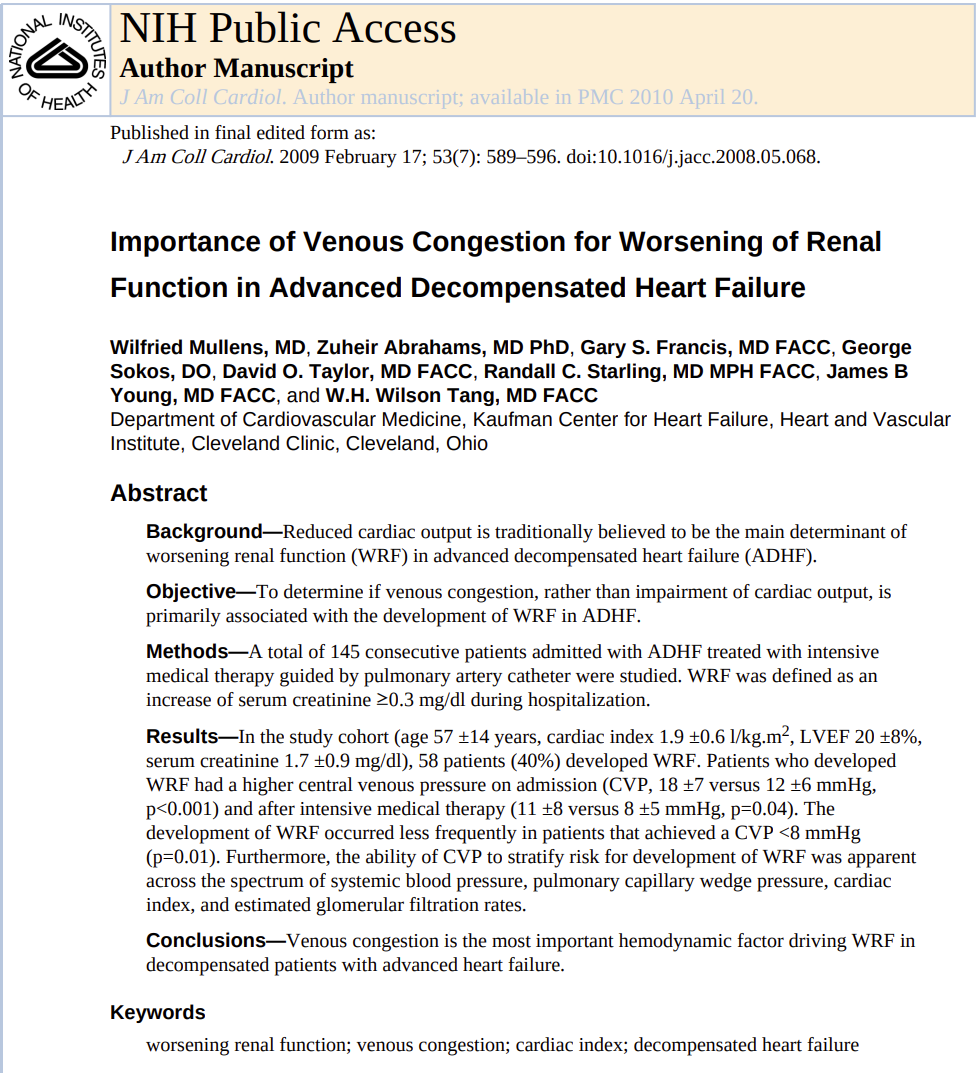
\includegraphics{ss_jurnal_metpen1.png}

}

\caption{screenshot Jurnal}

\end{figure}%

\subparagraph{Alasan
Association/causation:}\label{alasan-associationcausation}

Penelitian Mullens et al diatas meneliti hubungan antara kongesti vena
(CVP/central venous pressure) terhadap perburukan fungsi ginjal pada
pasien dewasa dengan ADHF. Pertanyaan penelitian ini adalah apakah
kongesti vena (diukur dengan kateter arteri pulmoner) merupakan faktor
yang berasosiasi dengan perburukan fungsi ginjal pada pasien ADHF.
Tujuan lainnya adalah menjawab apakah asosiasi tersebut lebih bermakna
dibandingkan asosiasi penurunan cardiac output (diukur dengan cardiac
index) terhadap penurunan fungsi ginjal, dimana secara umum teori yang
diterima adalah faktor utama perburukan fungsi ginjal pada ADHF adalah
penurunan cardiac output.

Penelitian ini cenderung mendukung \textbf{Causation} antara kongesti
vena dengan penurunan fungsi ginjal. Hal ini karena variabel independen
berkontribusi terhadap penurunan fungsi ginjal (ditemukan asosiasi
melalui perhitungan statistik). CVP ditemukan lebih tinggi baik saat
admisi dan setelah mendapatkan terapi ADHF secara intensif pada pasien
yang mengalami perburukan fungsi ginjal. Secara prospektif, ketika
pasien mendapatkan terapi ADHF dan CVP berhasil diturunkan \textless8
mmHg, pasien yang kemudian mengalami perburukan fungsi ginjal lebih
jarang ditemukan (mendukung prior association). \textbf{Causation yang
ditemukan merupakan contributory cause}. Terdapat beberapa variabel yang
bisa menjadi confounding karena tidak dilakukan pemeriksaan diantaranya
regional renal perfusion, kelainan struktural ginjal, serta analisis
data secara multivariabel tidak dilakukan

\subparagraph{Ide Penelitian
Selanjutnya:}\label{ide-penelitian-selanjutnya}

\textbf{Hubungan diameter dan collapsibility index inferior vena cava
terhadap perburukan fungsi ginjal pada pasien acute decompensated heart
failure.}

\section{Filsafat Ilmu Kedokteran}\label{filsafat-ilmu-kedokteran}

\subsubsection{Tugas Filsum-1 - Pengenalan filsafat
ilmu}\label{tugas-filsum-1---pengenalan-filsafat-ilmu}

\paragraph{Tugas/Pertanyaan/Instruksi}\label{tugaspertanyaaninstruksi-1}

Epistemology

\paragraph{Jawaban/Hasil}\label{jawabanhasil-1}

\section{Evidence-based Medicine}\label{evidence-based-medicine-1}

\subsubsection{Tugas EBM-1 - Introduction to EBM \& Critical
Appraisal}\label{tugas-ebm-1---introduction-to-ebm-critical-appraisal}

\paragraph{Tugas/Pertanyaan/Instruksi}\label{tugaspertanyaaninstruksi-2}

Instruksi : Membuat pertanyaan klinis berdasarkan prinsip PICO !

Skenario : Kita menghadapi anak dg defisiensi growth hormone (GH),
apakah pemberian terapi GH eksogen dapat memacu pertumbuhan anak
tersebut?

\paragraph{Jawaban/Hasil}\label{jawabanhasil-2}

\subparagraph{PICO}\label{pico}

P (patient/population) : Anak usia 2 - 14 tahun dengan isolated growth
hormone deficiency (GH)

I (intervention) : Terapi GH eksogen dengan dosis awal 25 mcg/kgBB/hari

C (comparison/control): plasebo

O (outcome) : laju peningkatan tinggi badan per tahun (\(\Delta\) height
velocity) \textgreater3 cm dalam 12 bulan terapi.

\subparagraph{Pertanyaan Klinis}\label{pertanyaan-klinis}

Pada pasien anak usia 2 -14 tahun dengan isolated growth hormone
deficiency, apakah pemberian growth hormone eksogen sebagai terapi dapat
meningkatkan \(\Delta\) height velocity \textgreater3 cm/tahun pada 12
bulan terapi dibandingkan anak yang diberikan terapi plasebo.

\subparagraph{Contekan}\label{contekan}

https://academic.oup.com/jcem/article/93/2/352/2597982
https://onlinelibrary.wiley.com/doi/10.1111/j.1365-2265.2012.04420.x
https://www.ncbi.nlm.nih.gov/pmc/articles/PMC6979443/

\bookmarksetup{startatroot}

\chapter*{References}\label{references}
\addcontentsline{toc}{chapter}{References}

\markboth{References}{References}

\phantomsection\label{refs}
\begin{CSLReferences}{1}{0}
\bibitem[\citeproctext]{ref-PK_2018}
Kawthalkar, Shirish M. 2018. \emph{Essentials of {Clinical}
{Pathology}}. jaypee.
\url{https://www.jaypeedigital.com/book/9789380704197}.

\bibitem[\citeproctext]{ref-knuth84}
Knuth, Donald E. 1984. {``Literate Programming.''} \emph{Comput. J.} 27
(2): 97--111. \url{https://doi.org/10.1093/comjnl/27.2.97}.

\bibitem[\citeproctext]{ref-harrison_2022}
Loscalzo, J, A Fauci, D Kasper, S Hauser, D Longo, and J Jameson. 2022.
\emph{Harrison's {Principles} of {Internal} {Medicine}, 21e}. 21st ed.
McGraw Hill.
\url{https://accesspharmacy.mhmedical.com/content.aspx?bookid=3095&sectionid=259856983}.

\bibitem[\citeproctext]{ref-marino}
Marino, Paul L. 2014. \emph{Marino's the ICU Book}. Lippincott Williams
\& Wilkins.

\end{CSLReferences}



\printindex

\end{document}
